% !TeX spellcheck = en_GB
\section{Large Scale Circulation} \label{sec:largeScale}
In the following the large scale circulation between \num{19} and \SI{26}{\dec} is analysed.
\\
In December 2016, the NAO was positive, with +\num{0.4}, and negative sea level pressure for the Iceland low \citep{shi_climate_2016} was monitored. Since extreme weather events are often related to positive NAO might this explain the incident of the extreme Christmas storm in 2016. 

\subsection*{\num{19} to \SI{20}{\dec}}
A precursor to extreme storm Urd was a high-pressure system over Scandinavia  and an occluded low to the proximate east of Iceland (\Cref{fig:DT19_00}, \subref{fig:GP19_00}). Over the coming \SI{36}{\hour} a confluence of events resulted in a suppressed tropopause and cold air over Haukeliseter: a filament of a cut off low to the south and cold air advection from the north-east (\Cref{fig:DT19_00}, \subref{fig:GP19_00}).
%%%%%%%%%%%%%%%%%%%%%%%%%%%%%%%%%%%%%%%%%%%%%%%%%%%%%%%%%%%%%%
\begin{figure}[!t]
	\centering
	%%% dyntropo %%%%
	\begin{subfigure}[b]{0.49\textwidth}
		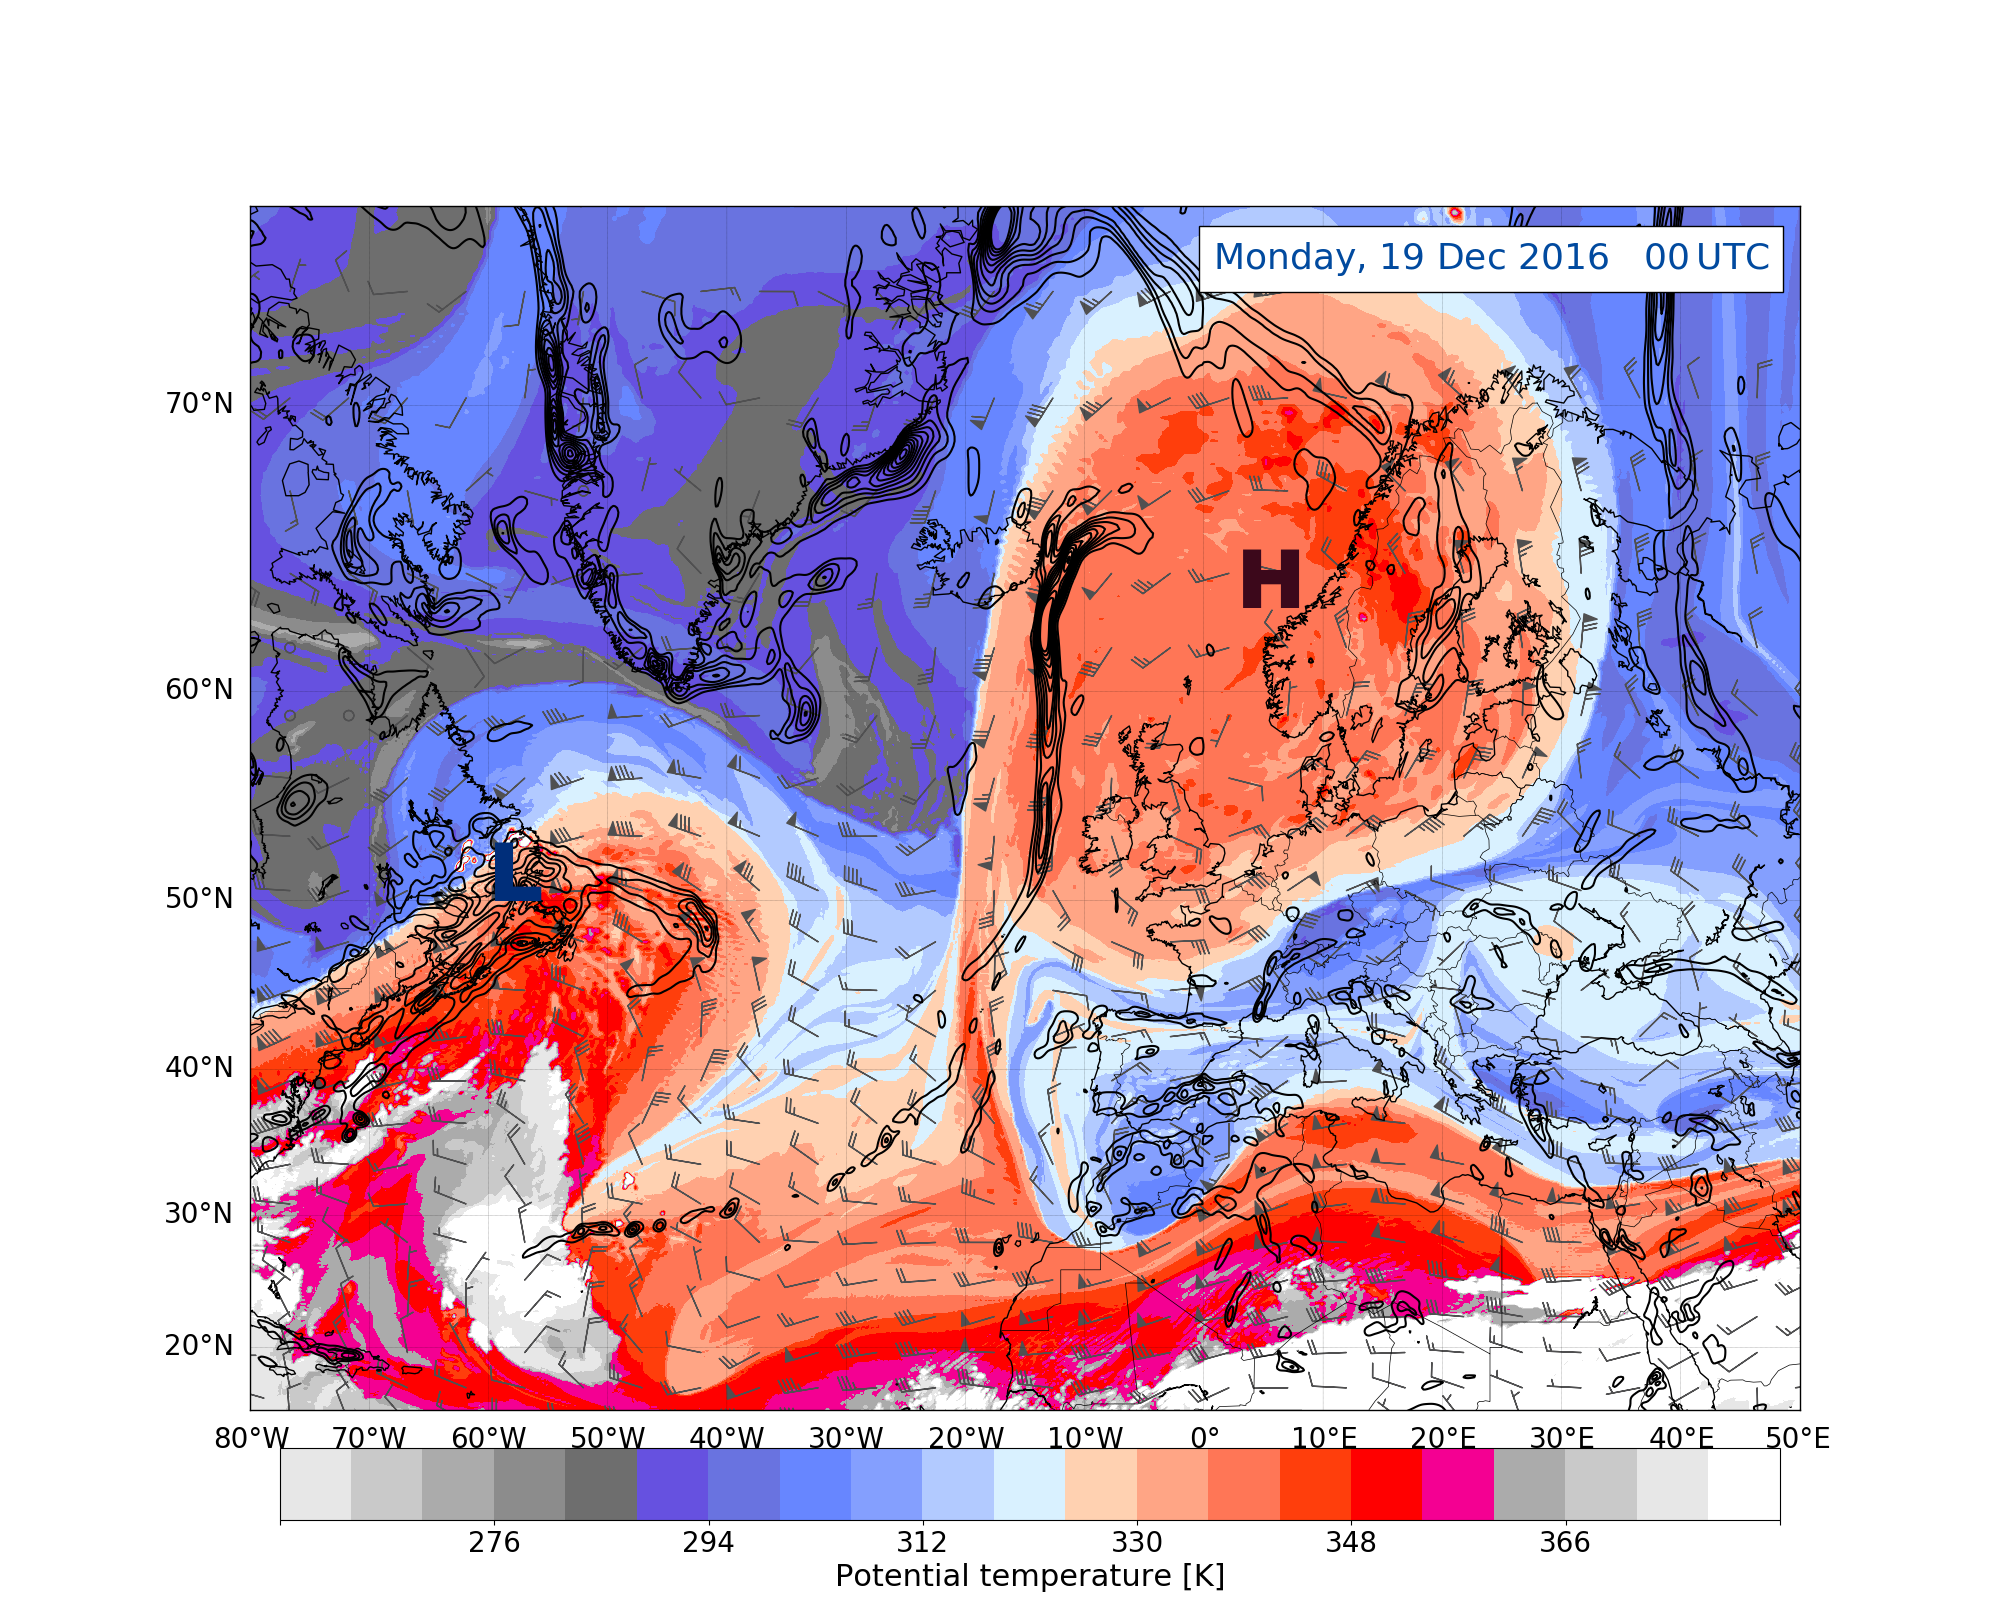
\includegraphics[trim={4.2cm 0cm 4.3cm 5.1cm},clip,
		width=\textwidth]{./fig_DynTropo/20161219_00}
		\caption{} \label{fig:DT19_00}
	\end{subfigure}
	%%% geopot %%%%
	\begin{subfigure}[b]{0.49\textwidth}
		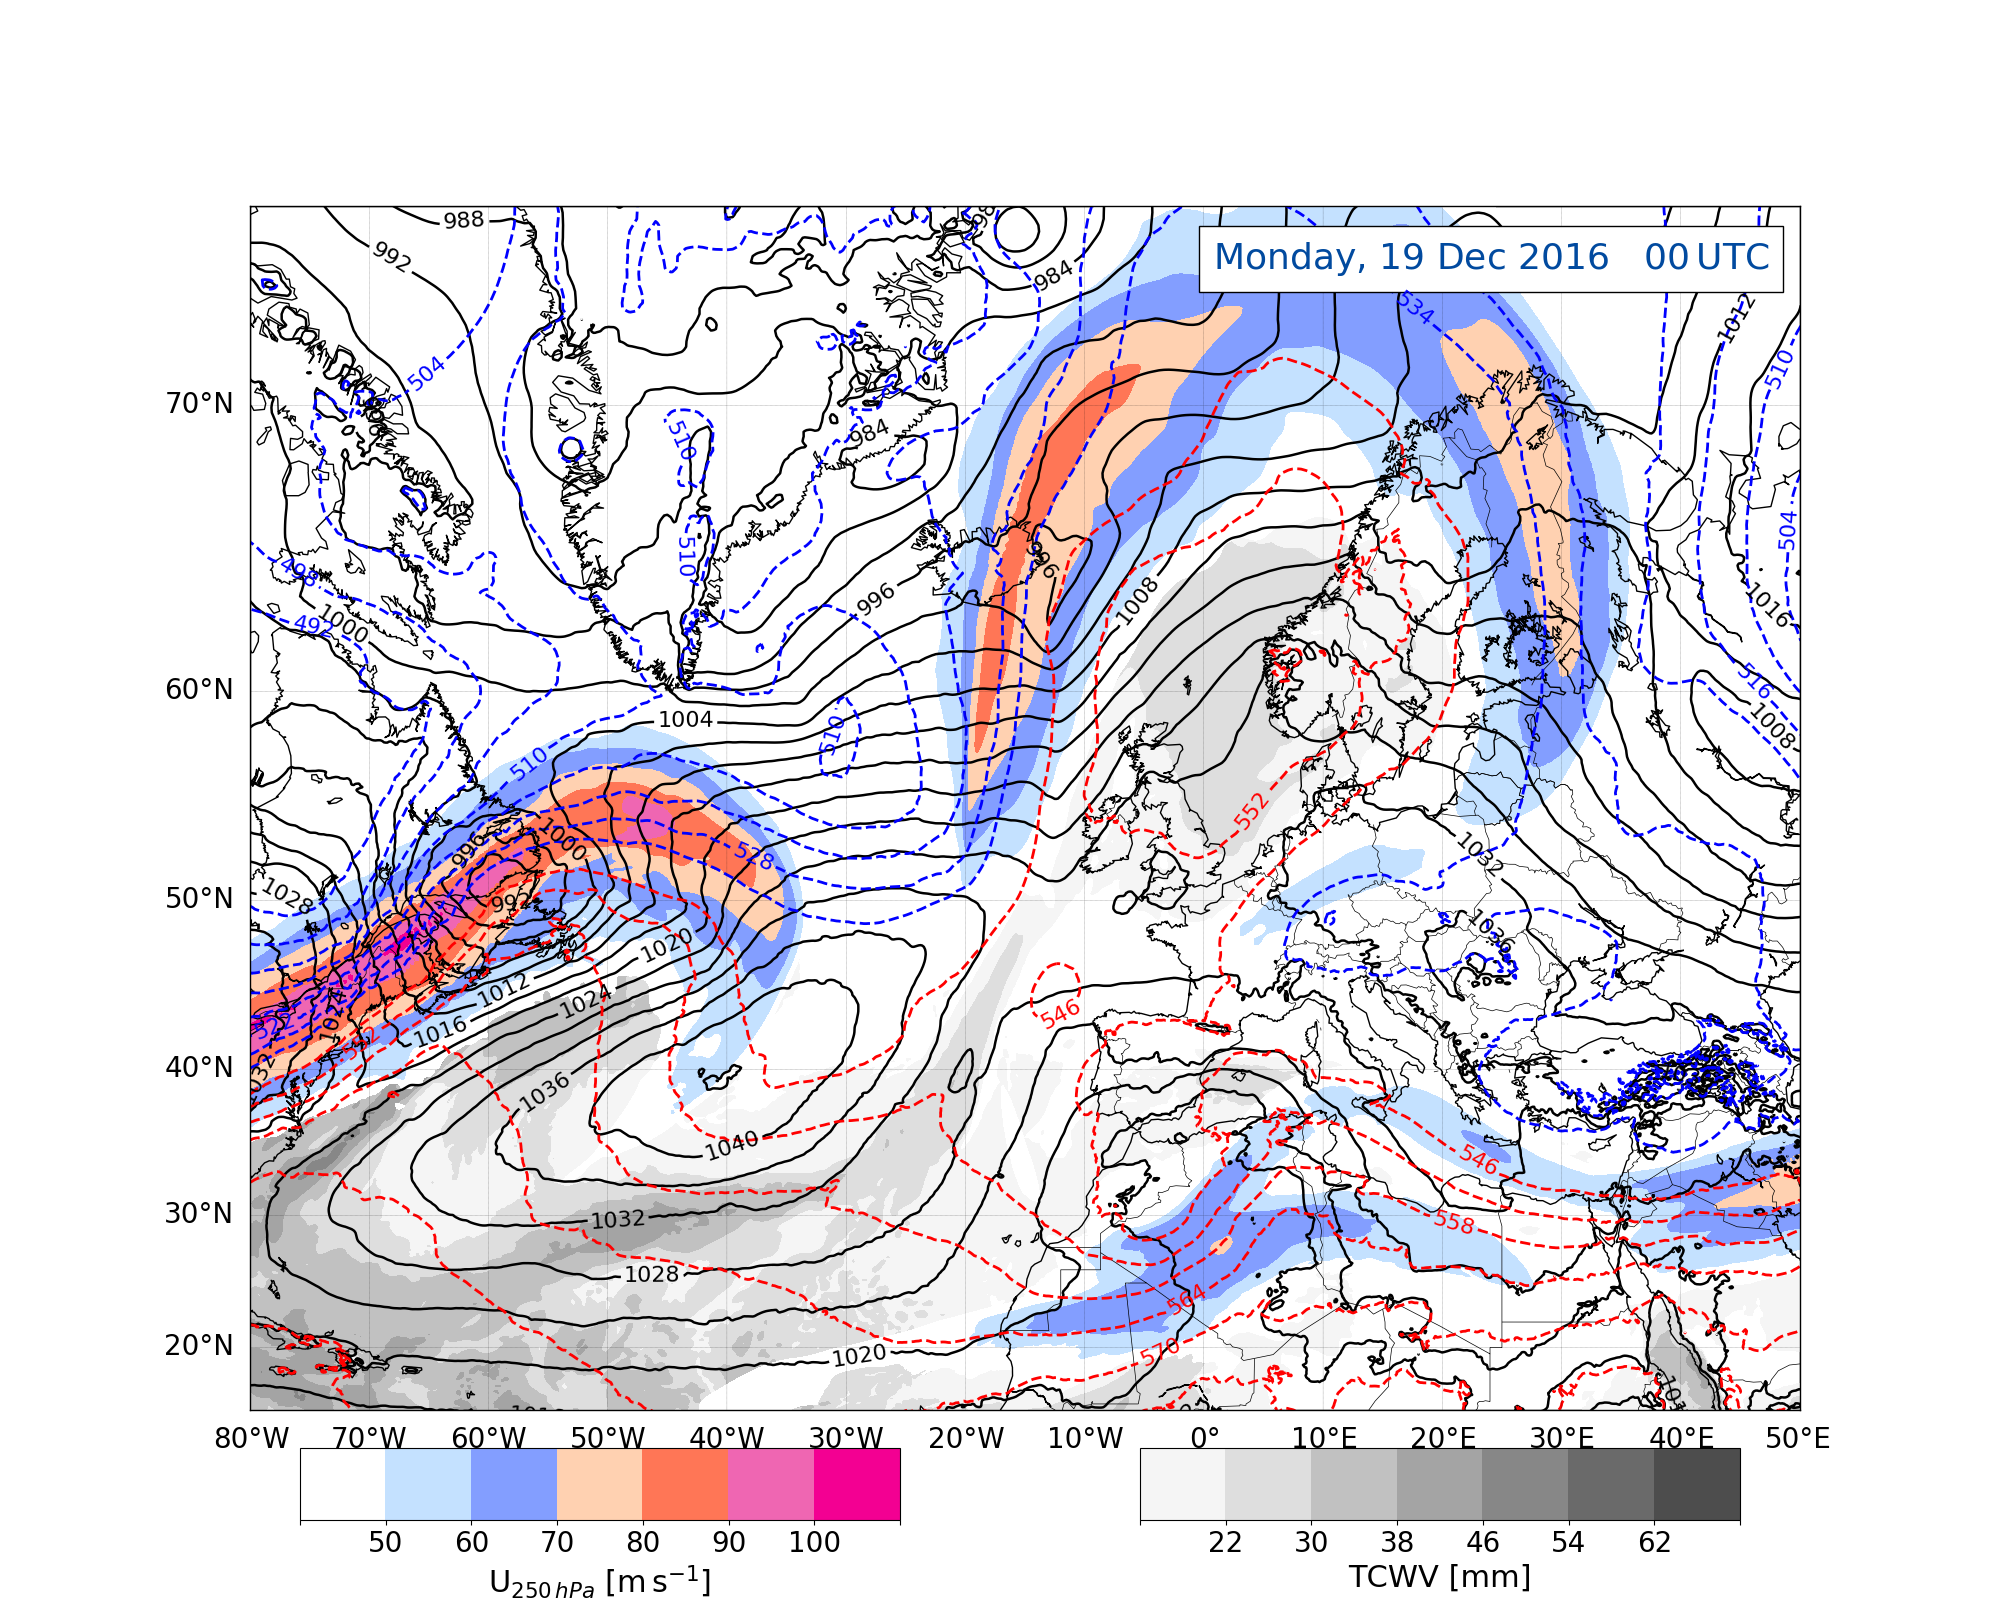
\includegraphics[trim={4.2cm 0cm 4.3cm 5.1cm},clip,
		width=\textwidth]{./fig_Geopot_Jet/20161219_00}
		\caption{} \label{fig:GP19_00}
	\end{subfigure}
	%%% local obs %%%%
	\begin{subfigure}[b]{0.49\textwidth}
		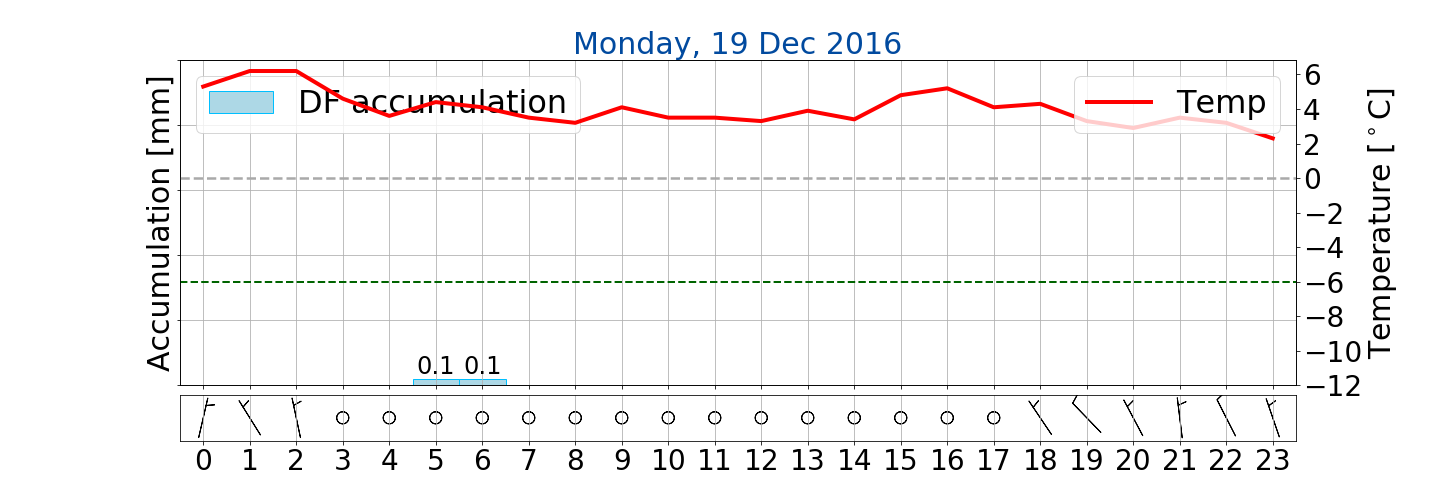
\includegraphics[trim={4.9cm 1.cm 1.5cm 1cm},clip,
		width=\textwidth]{./fig_weathermast/T_P_U_20161219}
		\caption{} \label{fig:TPU19}
	\end{subfigure}
	\caption{ECMWF analysis for dynamic tropopause (\protect\subref{fig:DT19_00}) as described in \Cref{sec:DT}, thickness map (\protect\subref{fig:GP19_00}) as evaluated in \Cref{sec:Geop}, and local observations (\protect\subref{fig:TPU19}) at Haukeliseter explained in \Cref{sec:loc_obs}). Analysis is shown for \SI{19}{\dec} at 0\SI{0}{\UTC}. Surface lows are indicated as \textbf{L} and surface highs as \textbf{H}. %\textit{Continued on next page.} 
	}\label{fig:weather:19}
\end{figure}
%%%%%%%%%%%%%%%%%%%%%%%%%%%%%%%%%%%%%%%%%%%%%%%%%%%%%%%%%%%%%%



%%% 21/12
% 21/00
% Westerly flow, perfect for orographic lifting
% → lots of moisture (check for correct values)
% Cold air goes right over Norway 
% → probably snow
% 21/18
% Low forming right at the main baroclinic zone (~45°N, south of Greenland)
% Formation @ the right entrance region of the jet, which helps for lifting
\subsection*{\SI{21}{\dec}}
Associated with the previously mentioned occluded cyclone, cold air impinges on Scandinavia on \SI{21}{\dec} (\Cref{fig:DT21}, \subref{fig:GP21}). Moisture is transported from the low latitudes to high latitudes, influencing Norways west coast. The westerly flow in \Cref{fig:GP21} is additionally conducive to orographic lifting. This is coincident with the onset of precipitation at Haukeliseter at \SI{10}{\UTC} on \SI{21}{\dec} (\Cref{fig:TPU21}). Furthermore, given the low temperatures, solid phase precipitation is observed.
\\
Additionally, cyclogenesis is observed off the east coast of the United States (as evidenced by a trough to the northwest of low-level averaged relative vorticity.) 
%%%%%%%%%%%%%%%%%%%%%%%%%%%%%%%%%%%%%%%%%%%%%%%%%%%%%%%%%%%%%%
\begin{figure}[!t]
	\centering
	%%% dyntropo %%%%
	\begin{subfigure}[b]{0.49\textwidth}
		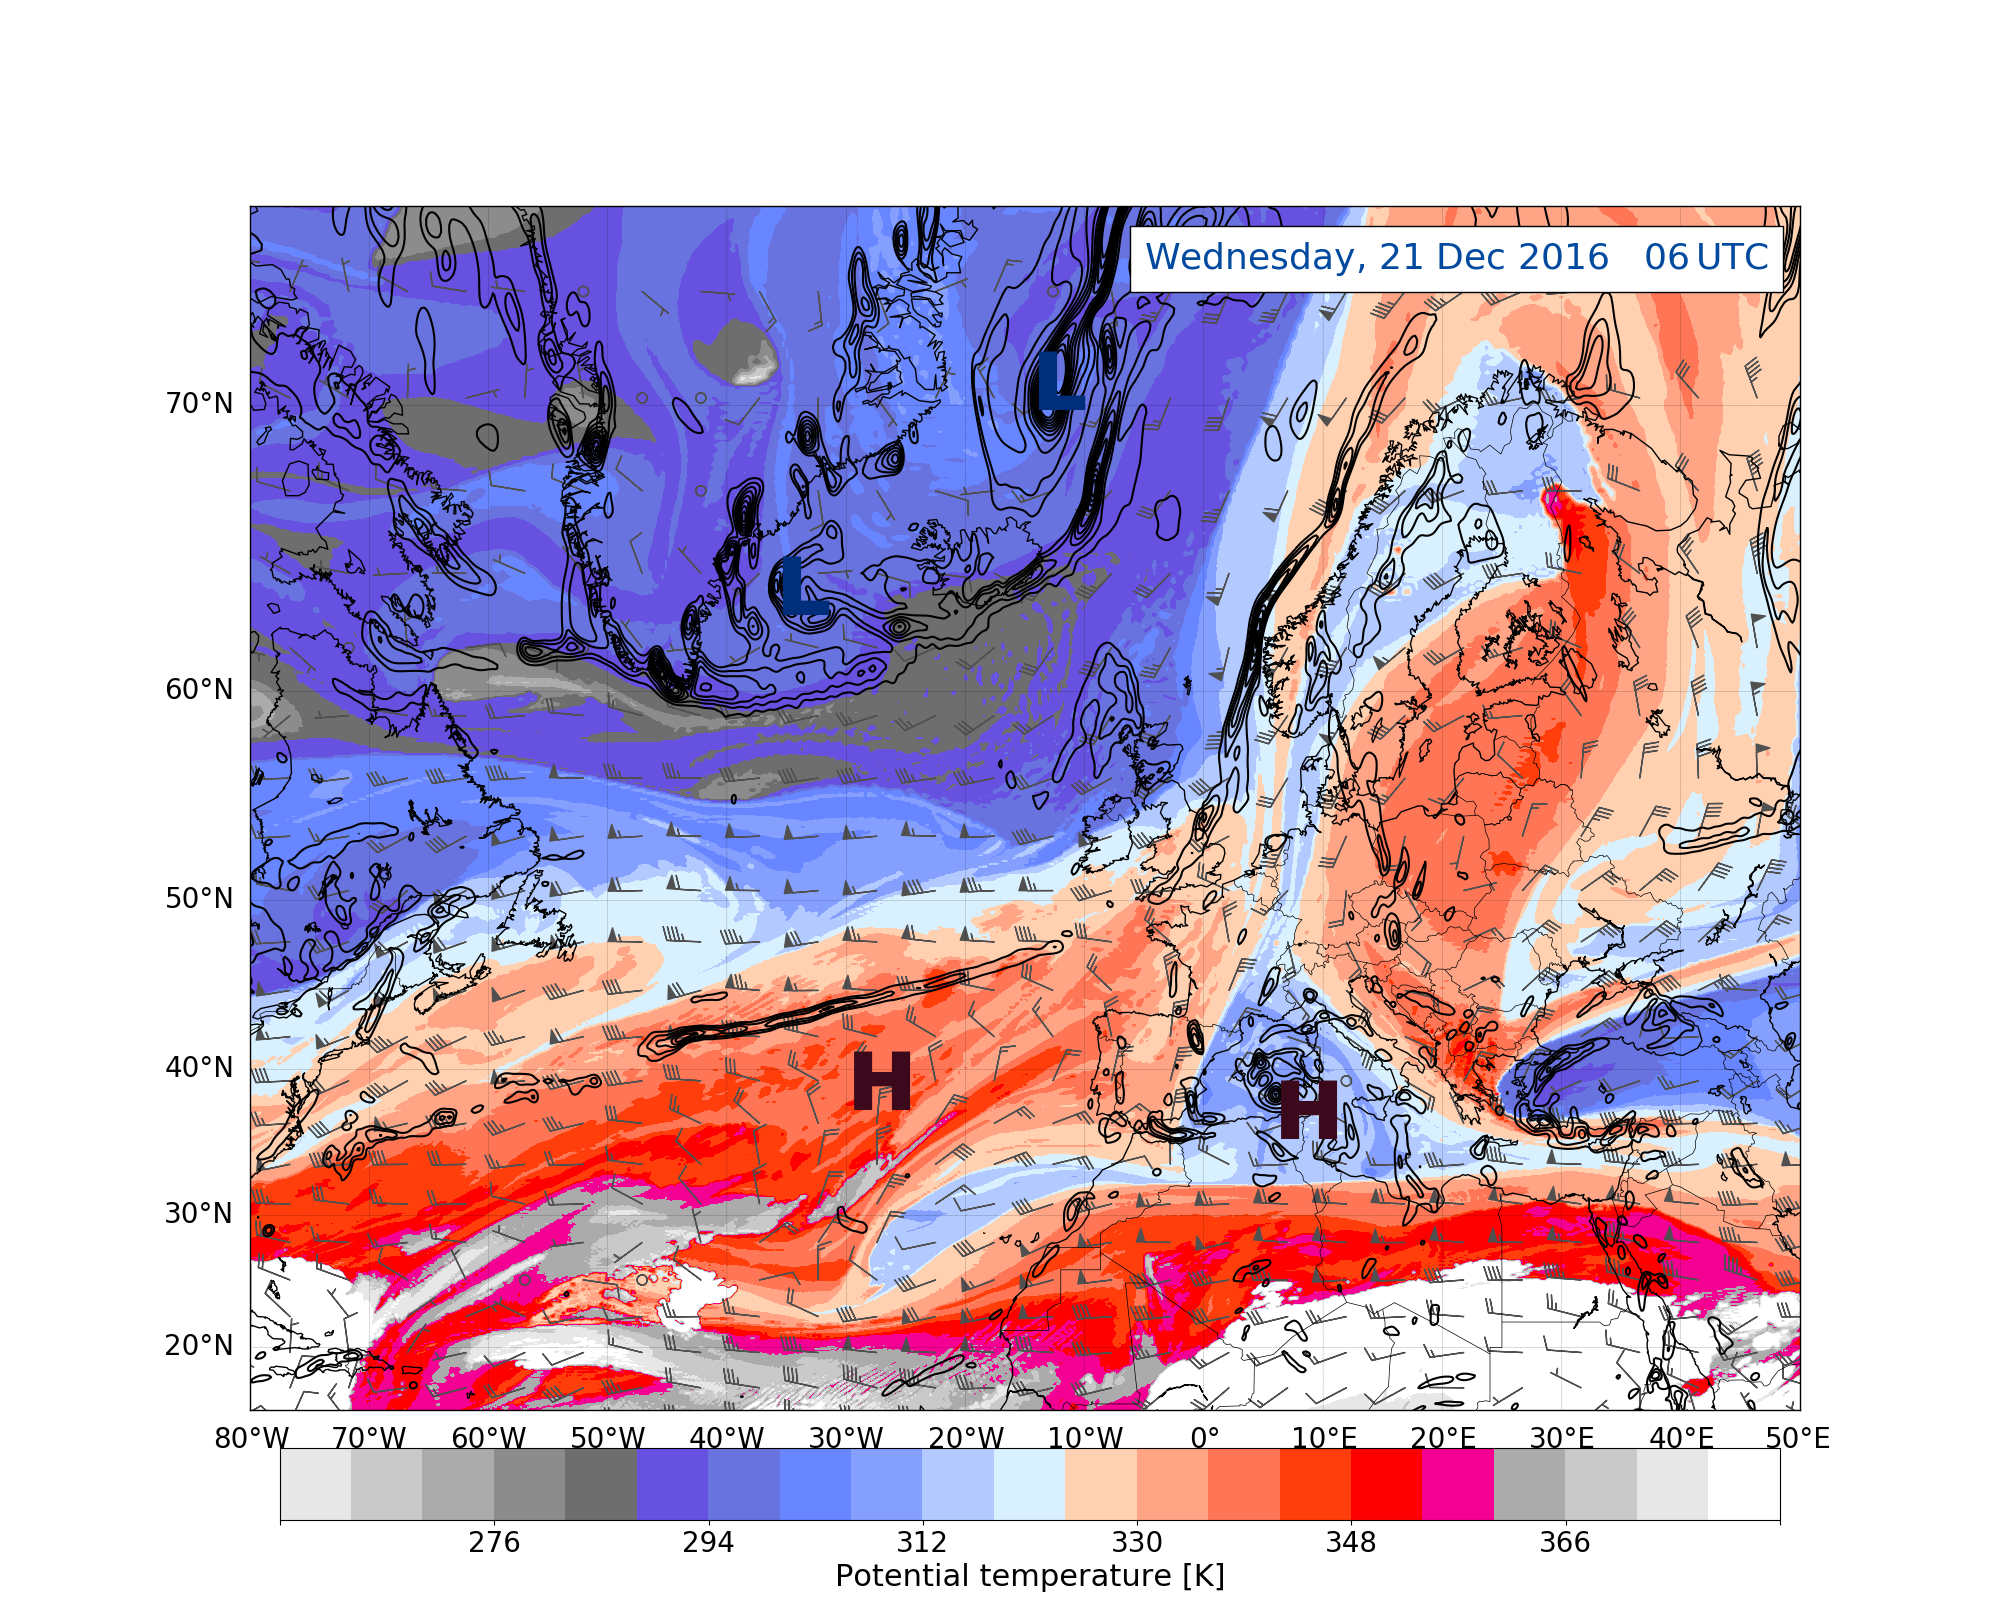
\includegraphics[trim={4.2cm 0cm 4.3cm 5.1cm},clip,
		width=\textwidth]{./fig_DynTropo/20161221_06}
		\caption{} \label{fig:DT21_06}
	\end{subfigure}
	\begin{subfigure}[b]{0.49\textwidth}
		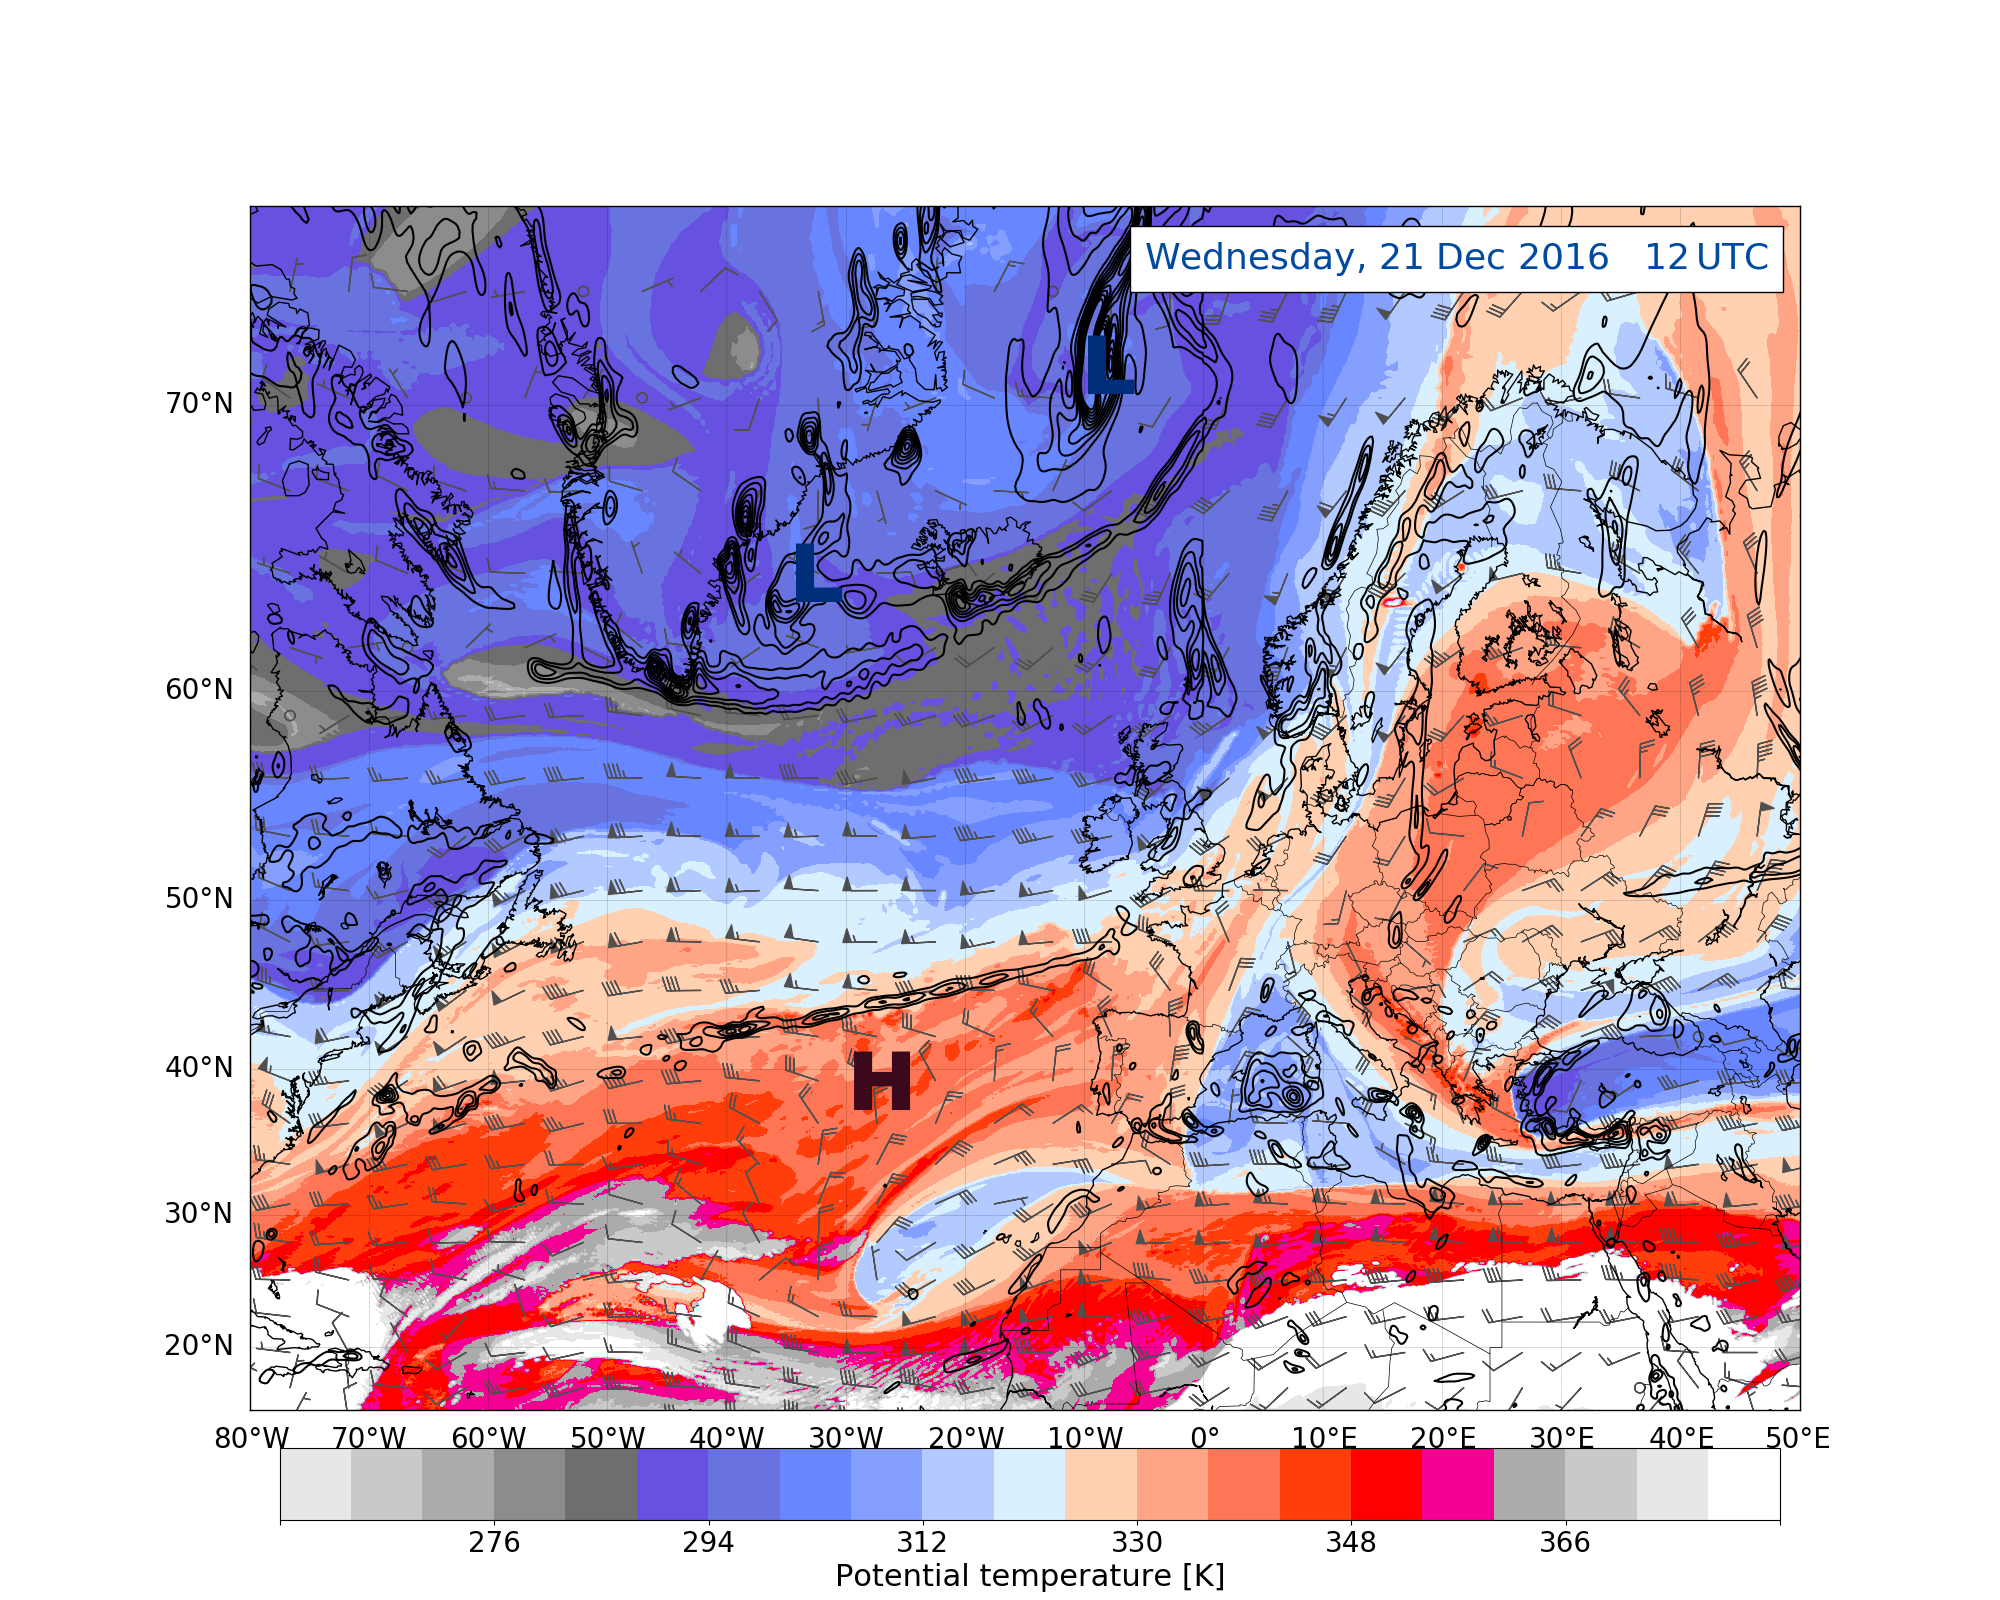
\includegraphics[trim={4.2cm 0cm 4.3cm 5.1cm},clip,
		width=\textwidth]{./fig_DynTropo/20161221_12}
		\caption{} \label{fig:DT21}
	\end{subfigure}
	%%% geopot %%%%
	\begin{subfigure}[b]{0.49\textwidth}
		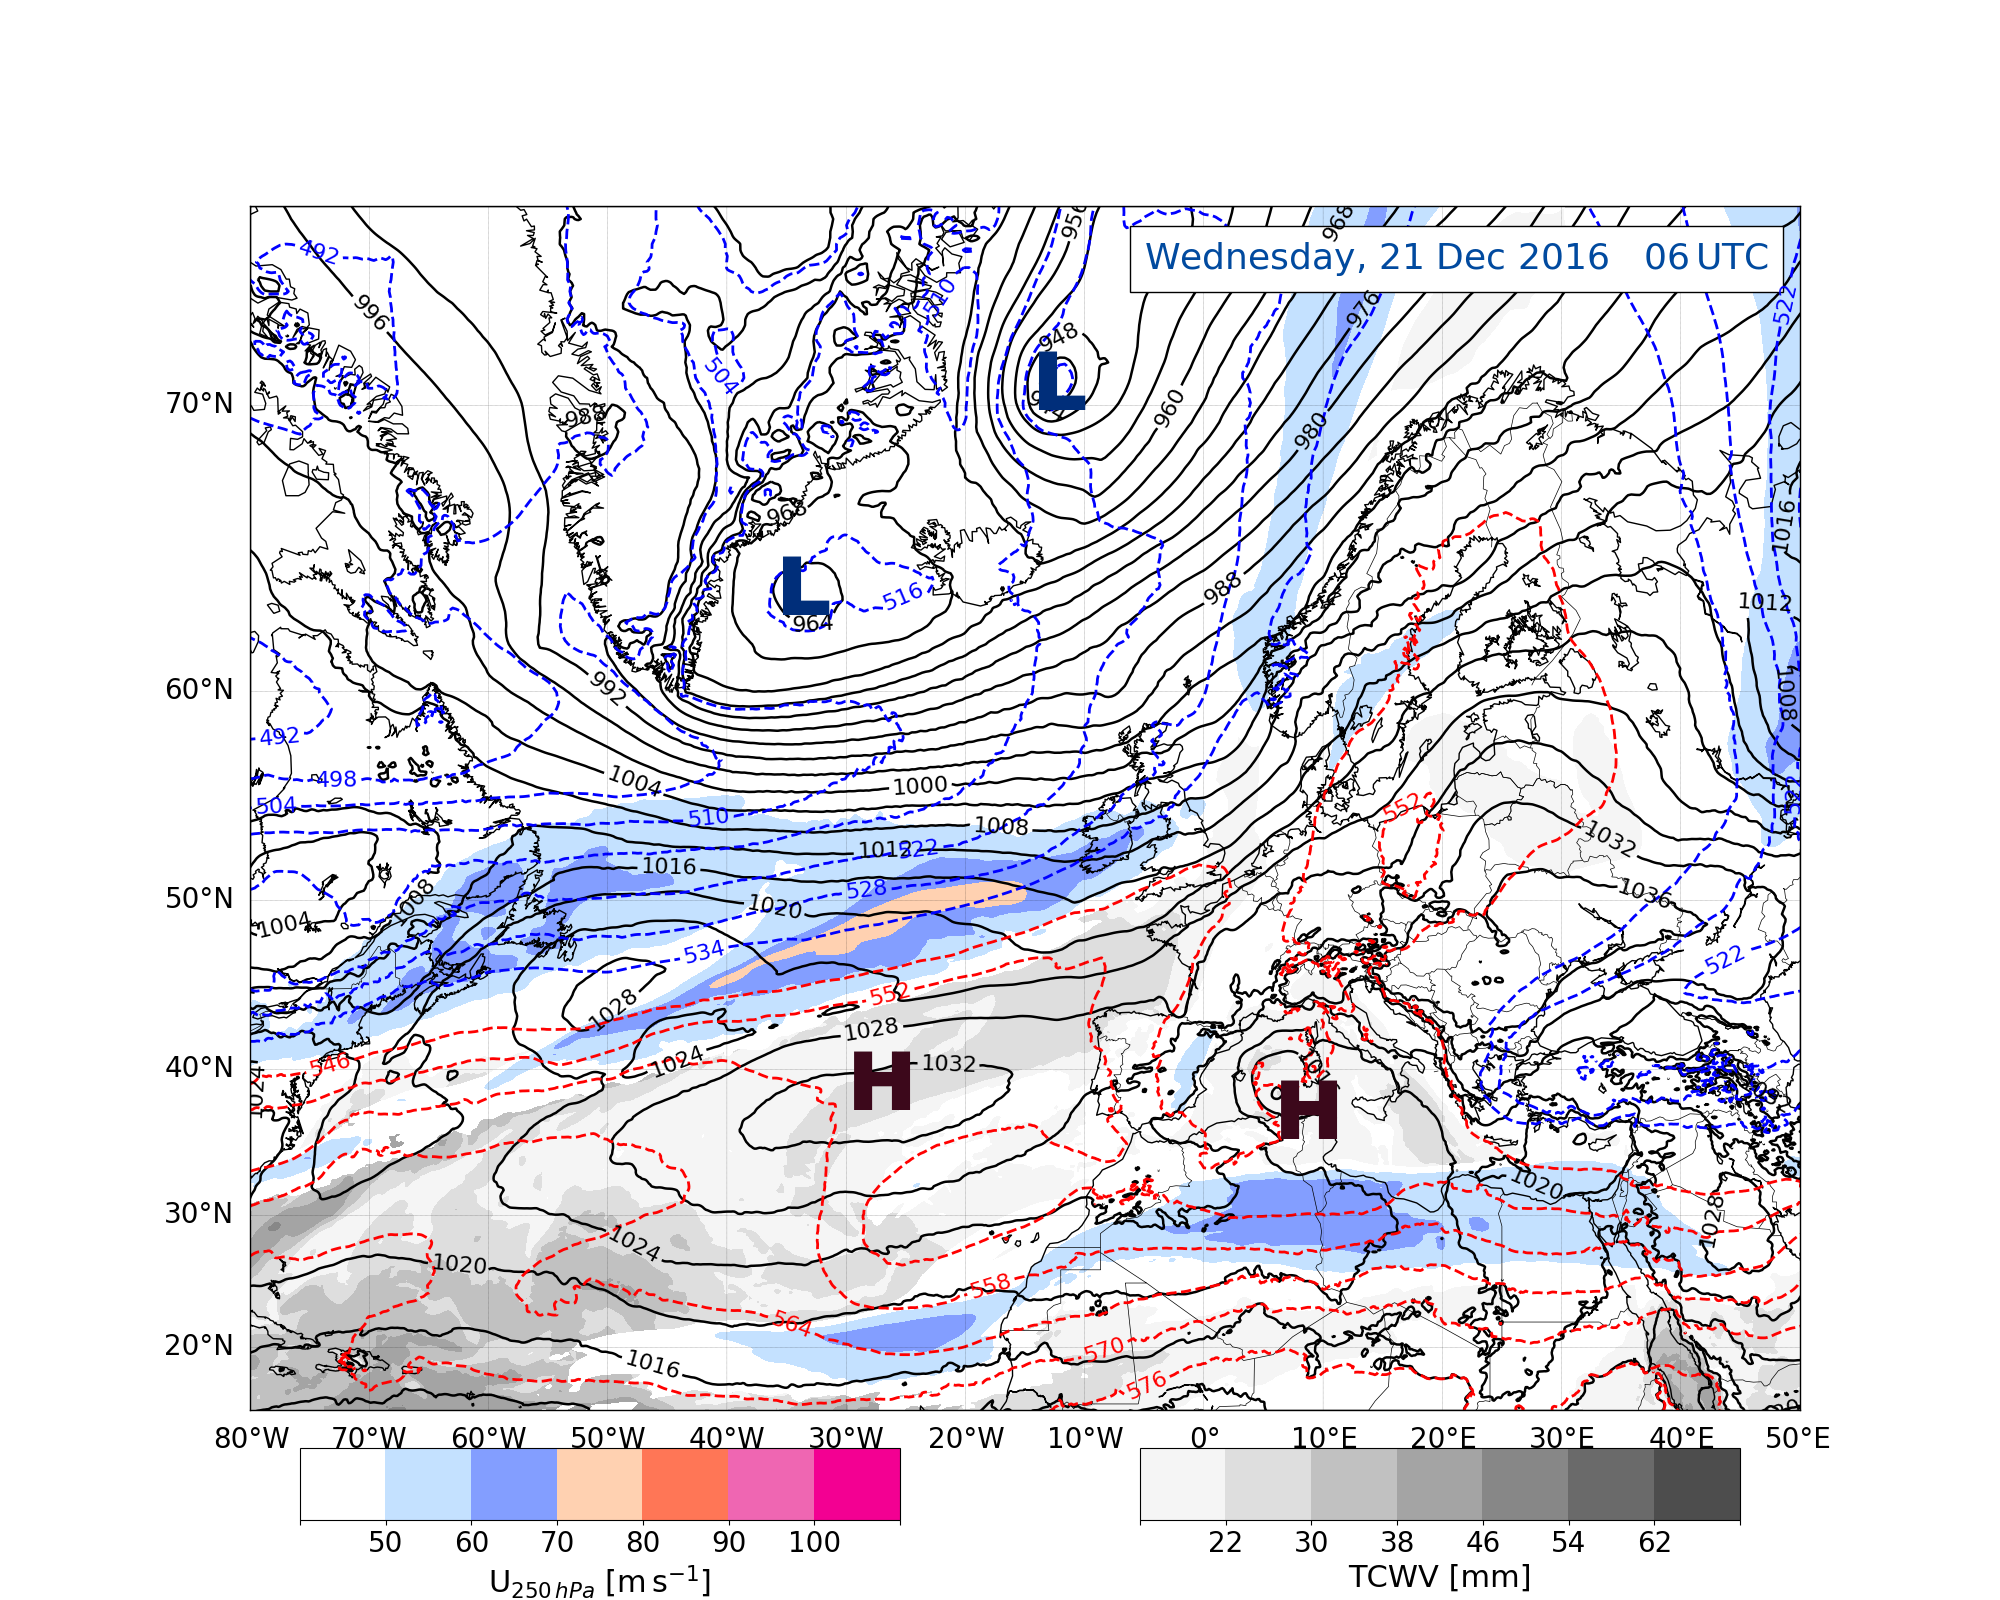
\includegraphics[trim={4.2cm 0cm 4.3cm 5.1cm},clip,
		width=\textwidth]{./fig_Geopot_Jet/20161221_06}
		\caption{} \label{fig:GP21_06}
	\end{subfigure}
	\begin{subfigure}[b]{0.49\textwidth}
		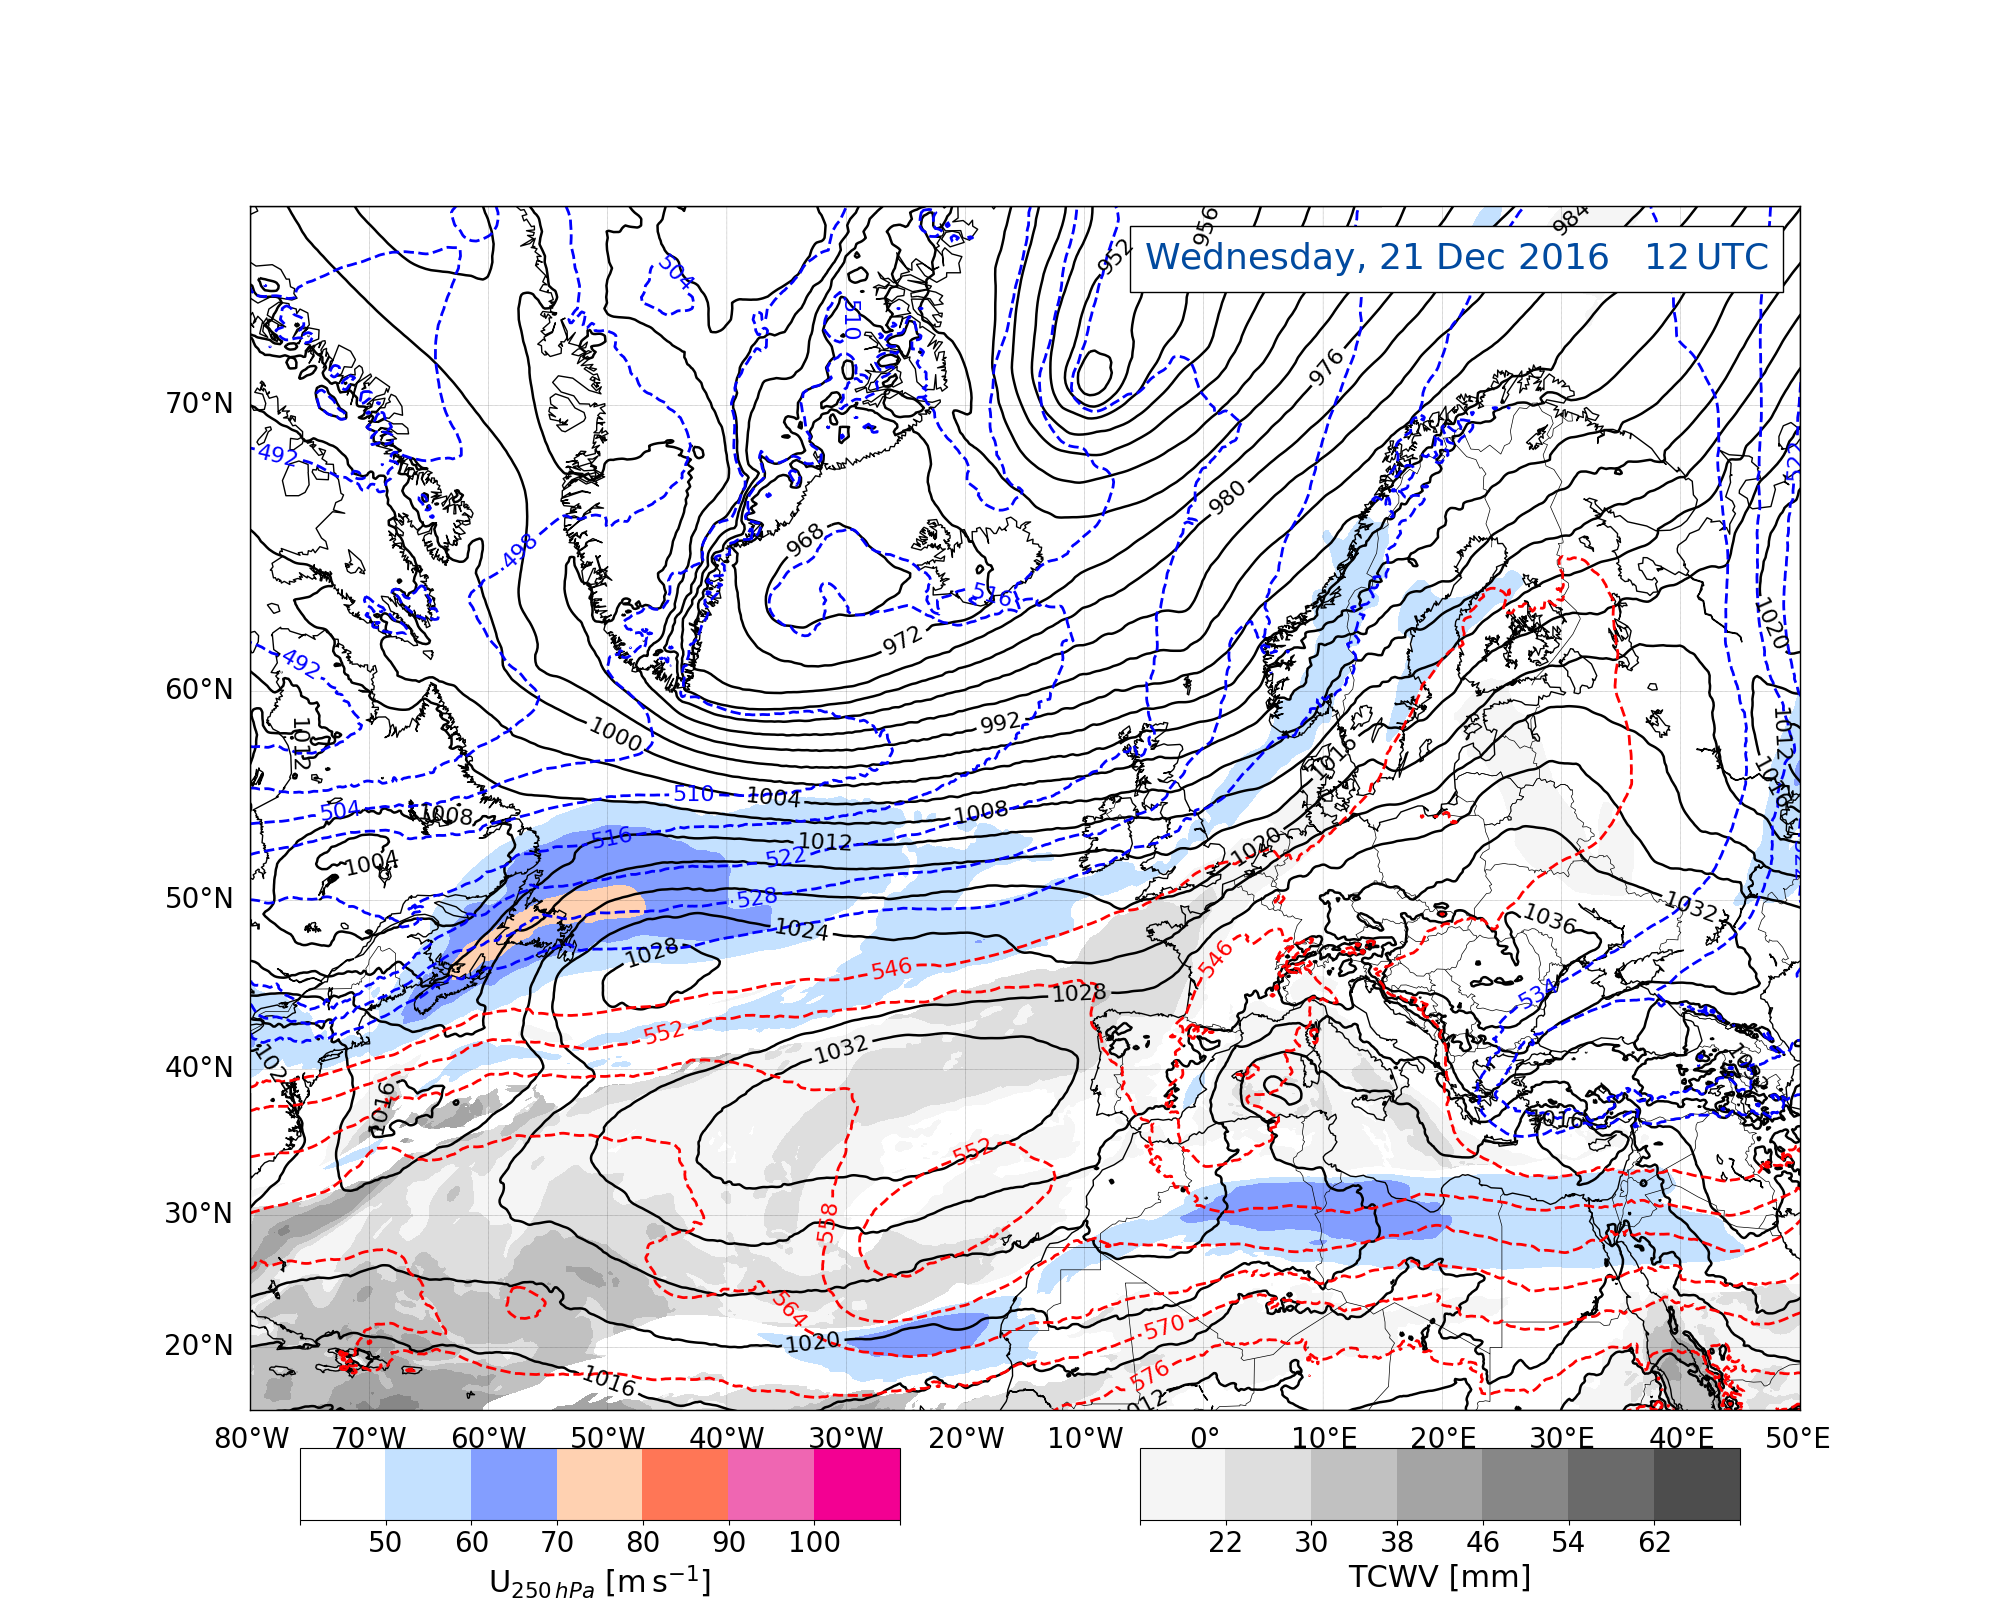
\includegraphics[trim={4.2cm 0cm 4.3cm 5.1cm},clip,
		width=\textwidth]{./fig_Geopot_Jet/20161221_12}
		\caption{} \label{fig:GP21}
	\end{subfigure}
	%%% local obs %%%%
	\begin{subfigure}[b]{0.49\textwidth}
		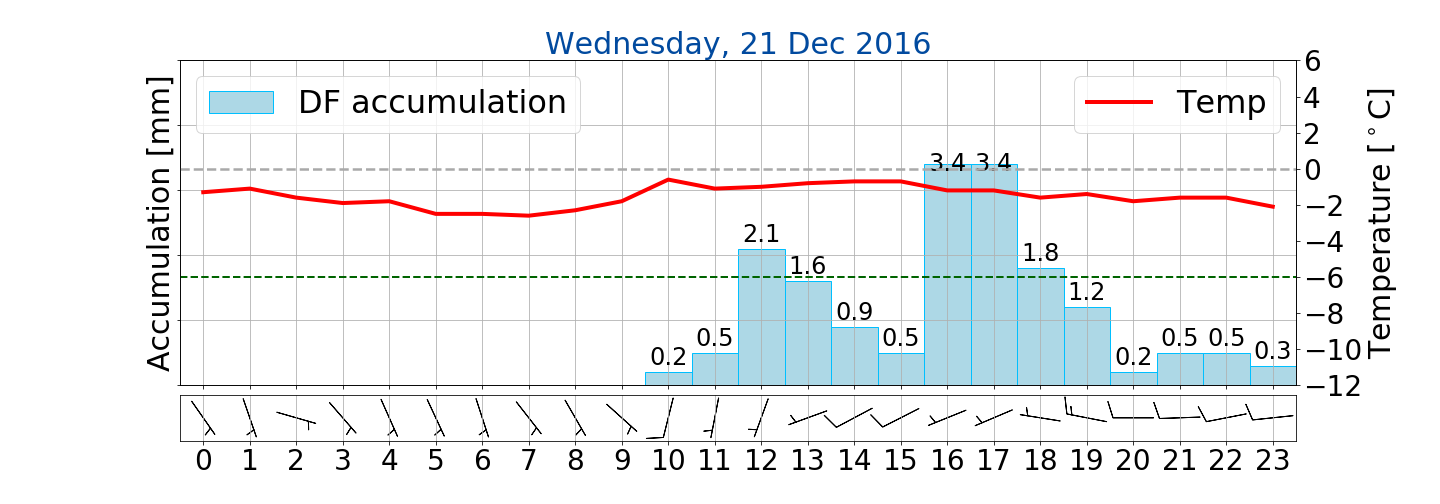
\includegraphics[trim={4.9cm 1.cm 1.5cm 1cm},clip,
		width=\textwidth]{./fig_weathermast/T_P_U_20161221}
		\caption{} \label{fig:TPU21}
	\end{subfigure}
	\caption{\textit{(As \Cref{fig:weather:19}.)} For \SI{21}{\dec} at \SI{06}{\UTC} (\protect\subref{fig:DT21_06}, \protect\subref{fig:GP21_06}) and at \SI{12}{\UTC} (\protect\subref{fig:DT21}, \protect\subref{fig:GP21}).}\label{fig:weather:21}
\end{figure}
%%%%%%%%%%%%%%%%%%%%%%%%%%%%%%%%%%%%%%%%%%%%%%%%%%%%%%%%%%%%%%


\clearpage
\subsection*{\SI{22}{\dec}}
%%% 22/12
% 22/12
% @ DT, phasing of the vorticity
% → low center is in perfect condition for synoptic scale lifting
% \noindent Twenty-four hours later the analysis shows from \SI{22}{\dec} phasing between the surface relative vorticity and the baroclinic zone at \ang{50}{\,N} in the DT. The centre of the surface low is directly located below the temperature gradient at the \SI{2}{PVU} surface, hence this is good for synoptic lifting. Furthermore, the strongest baroclinicity is observed on the south west side of the surface low.
% The synoptic map of the geopotential thickness and the surface pressure show the beginning of the frontal boundaries in \Cref{fig:GP22}. 
% At the same time shows the AR map, \Cref{fig:AR22}, large values just at the baroclinic zone, where the low pressure is beginning to form. \textcolor{red}{Help?! Does that lead to even more lifting in this area? Or does it just mean that the cyclone gets a good amount of moisture?!}.
% Norway is located in a cold area. The continues precipitation observed at Haukeliseter (\Cref{fig:TPU22}) is associated with the westerly flow which is conducive to orographic lifting, and therefore moisture release.  
Twenty-four hours later the analysis from \SI{22}{\dec} shows cold air remaining over Scandinavia (\Cref{fig:DT22}, \subref{fig:GP22}). Continues frozen precipitation is observed at Haukeliseter (\Cref{fig:TPU22}).
\\
The previously mentioned cyclone is observed to intensify during this time period along the baroclinic zone. The upper-level trough to the north-east of the low-level cyclone centre represents an optimal configuration for cyclone development, since the surface low is located below the temperature gradient at the \SI{2}{PVU} surface (\Cref{fig:DT22}, \subref{fig:GP22}). This is apparent in the intensification of the surface system (low-level averaged vorticity and mean sea level pressure minima) at \ang{50}{\,N}.  Also, in evidence is the diabatic ridging associated with the ascending warm conveyor belt air-stream (see warm colours in \Cref{fig:DT22}).
%%%%%%%%%%%%%%%%%%%%%%%%%%%%%%%%%%%%%%%%%%%%%%%%%%%%%%%%%%%%%%
\begin{figure}[ht!]%\ContinuedFloat
	\centering
	%%% dyntropo %%%%
	\begin{subfigure}[b]{0.49\textwidth}
		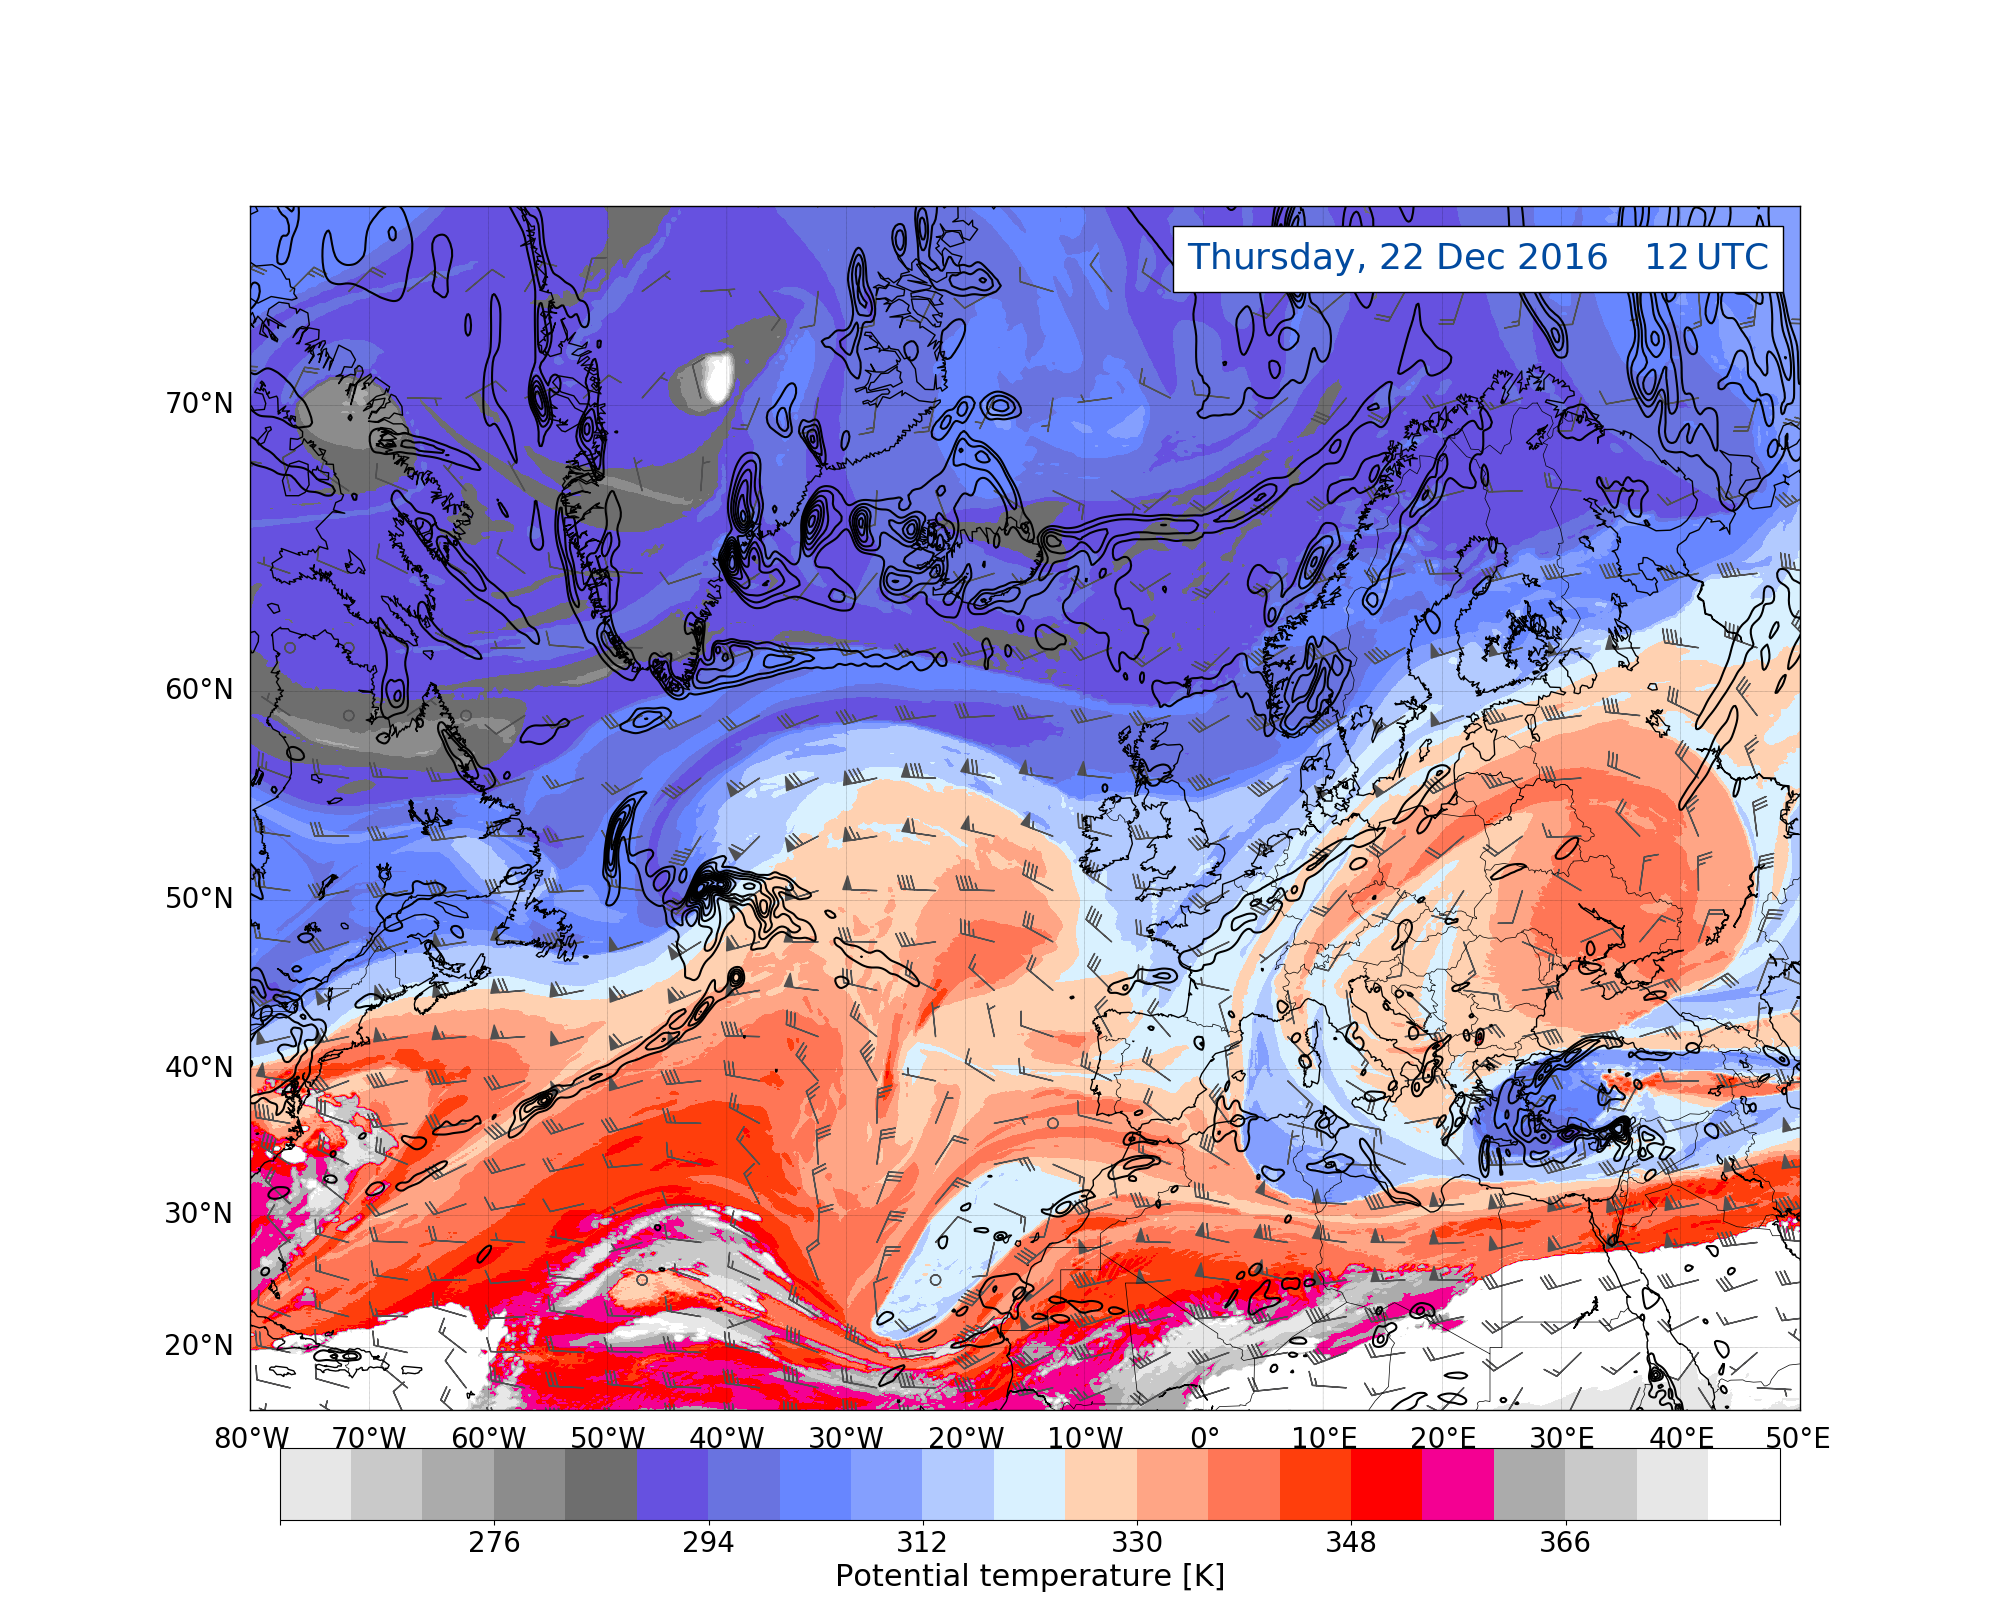
\includegraphics[trim={4.2cm 0cm 4.3cm 5.1cm},clip,
		width=\textwidth]{./fig_DynTropo/20161222_12}
		\caption{} \label{fig:DT22}
	\end{subfigure}
	%%% geopot %%%%
	\begin{subfigure}[b]{0.49\textwidth}
		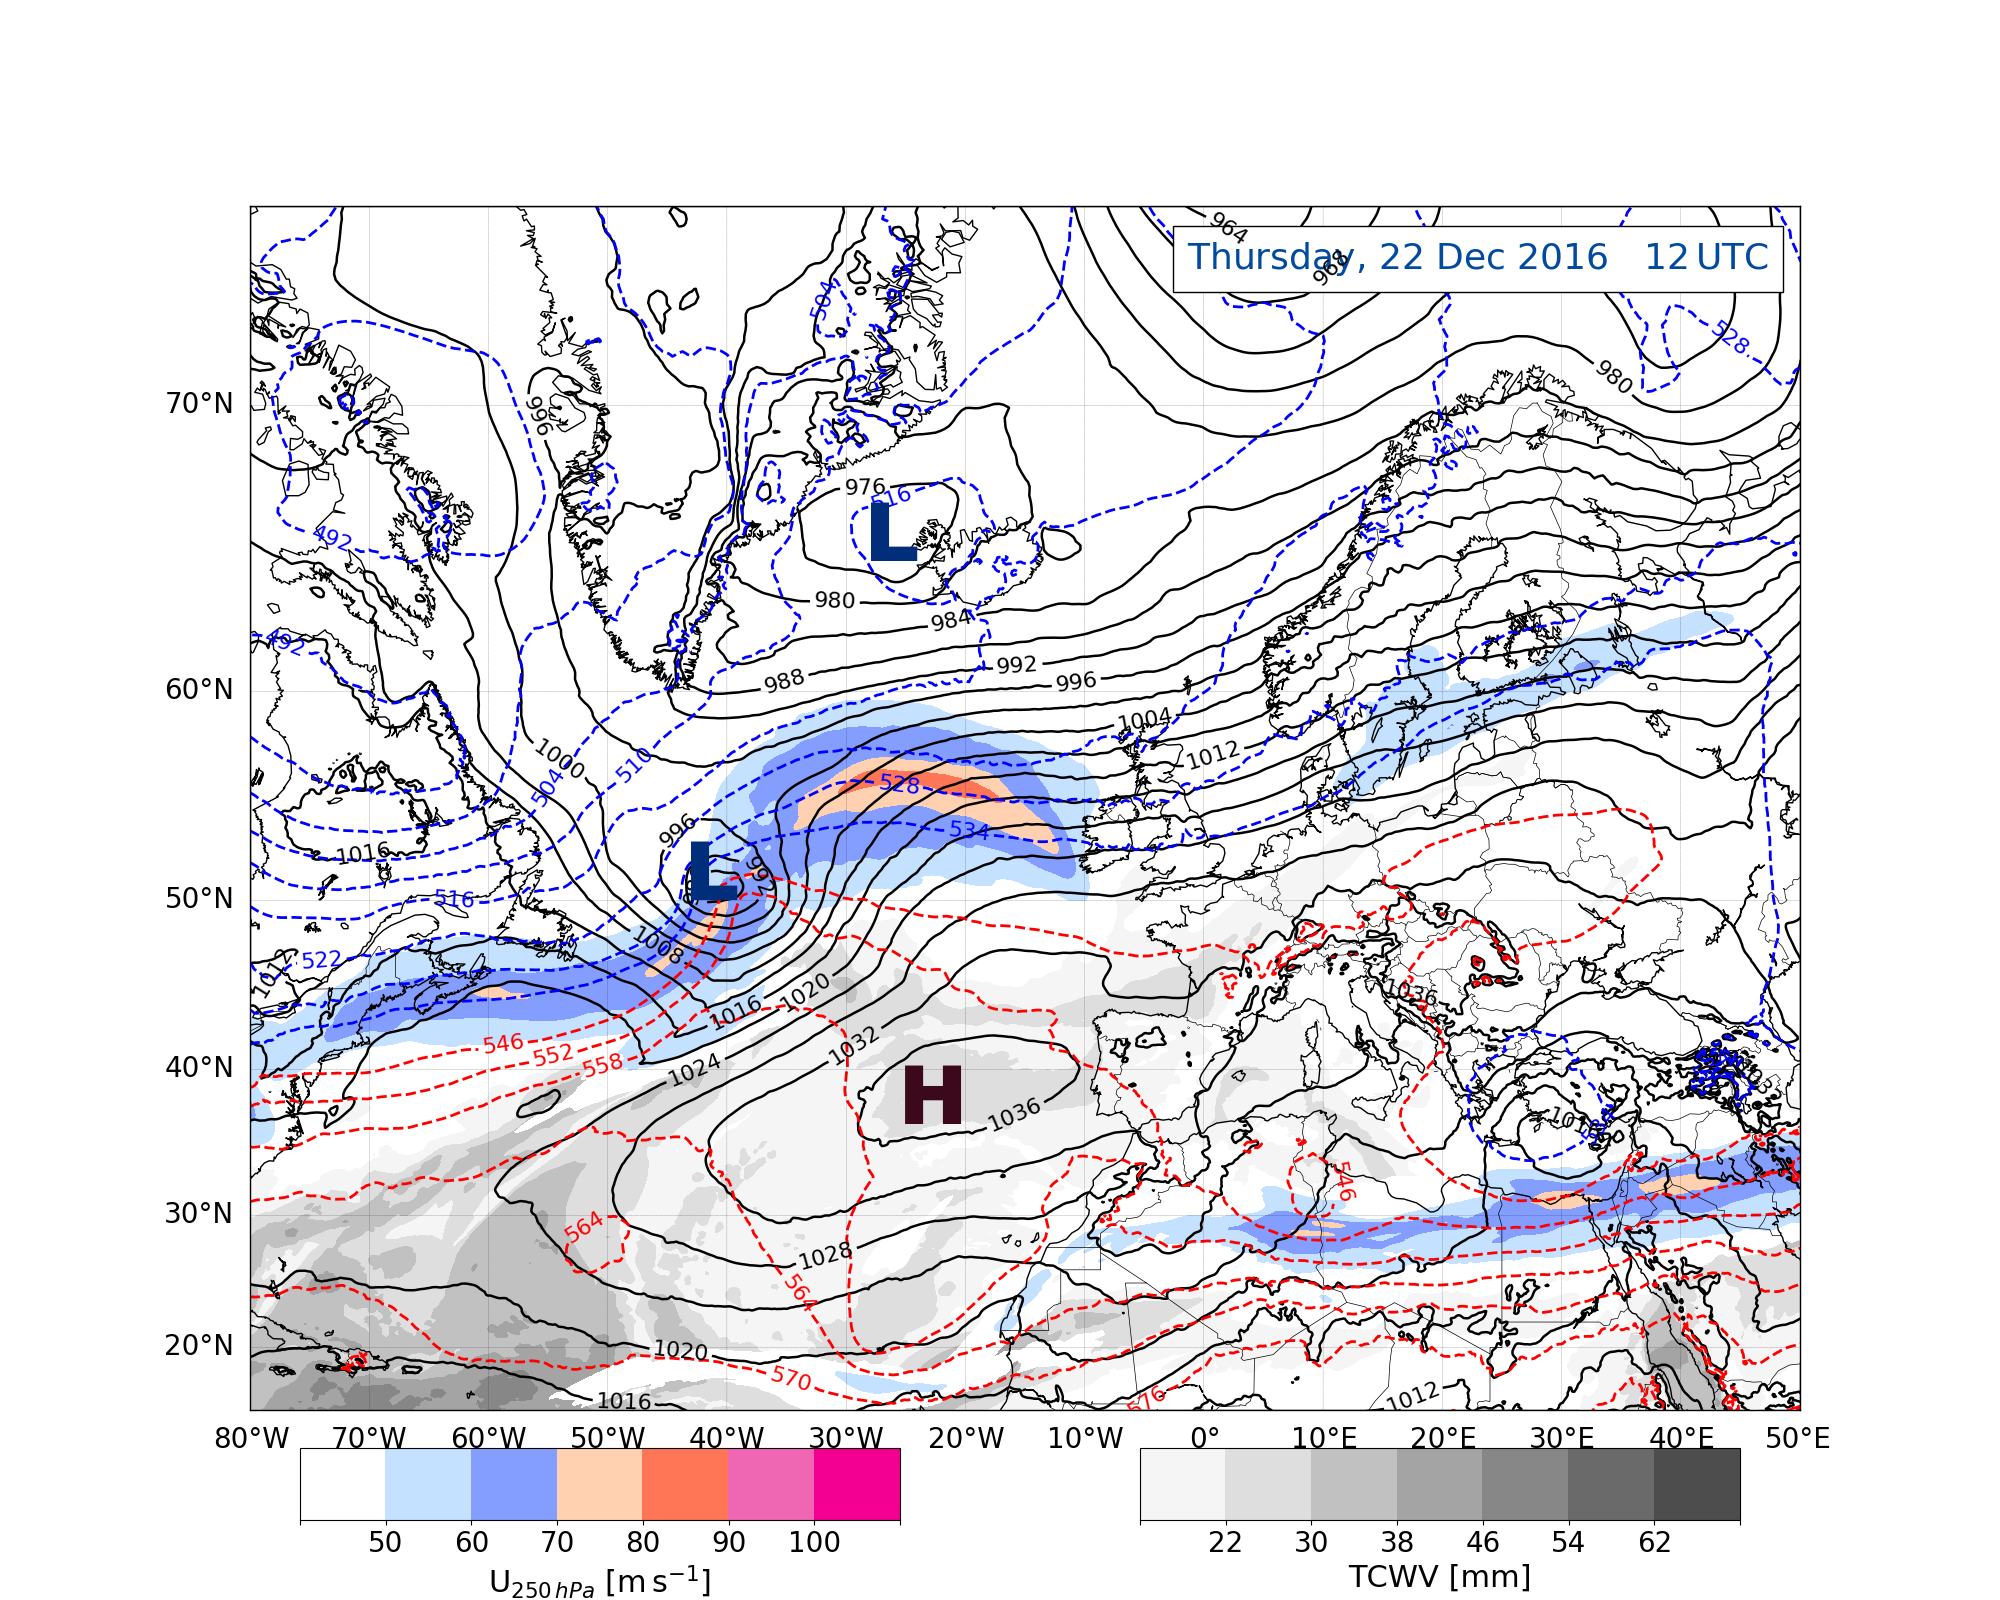
\includegraphics[trim={4.2cm 0cm 4.3cm 5.1cm},clip,
		width=\textwidth]{./fig_Geopot_Jet/20161222_12}
		\caption{} \label{fig:GP22}
	\end{subfigure}
	%%% local obs %%%%
	\begin{subfigure}[b]{0.49\textwidth}
		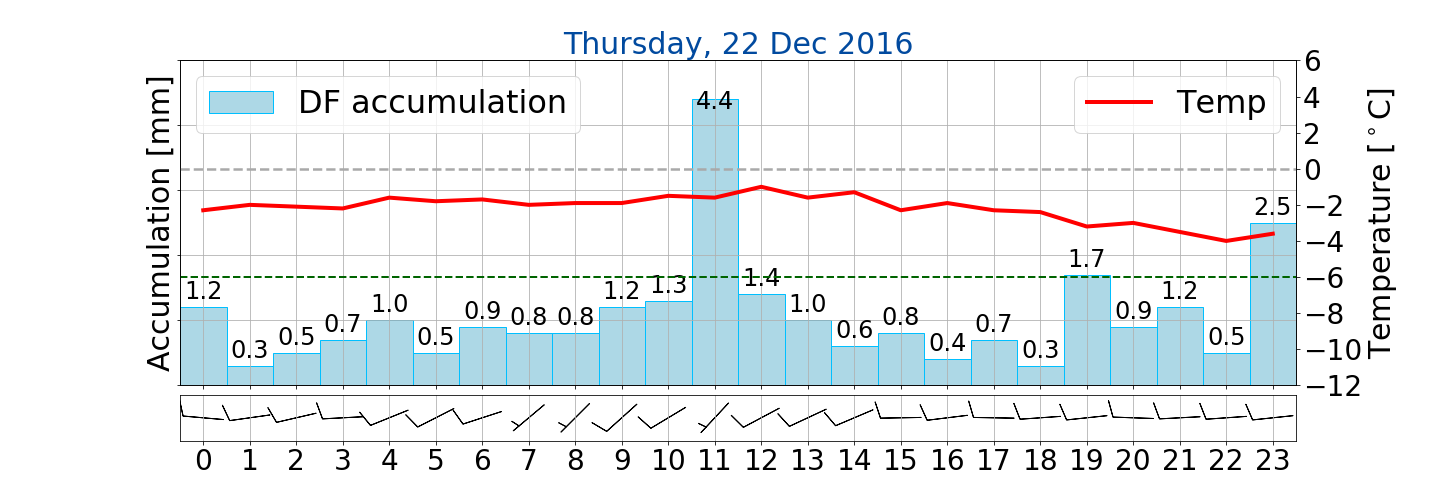
\includegraphics[trim={4.9cm 1.cm 1.5cm 1cm},clip,
		width=\textwidth]{./fig_weathermast/T_P_U_20161222}
		\caption{} \label{fig:TPU22}
	\end{subfigure}
	\caption{\textit{(As \Cref{fig:weather:19}.)} For \SI{22}{\dec} at \SI{12}{\UTC}.}\label{fig:weather:22}
\end{figure}
%%%%%%%%%%%%%%%%%%%%%%%%%%%%%%%%%%%%%%%%%%%%%%%%%%%%%%%%%%%%%%
\newpage
\subsection*{\SI{23}{\dec}}
%%% 23/12
% 23/06
% Still conducive westerly flow → orographic lifting
% Norway in cold area
% Jet not very strong
% Probably frozen precipitation
% Baroclinicity strongest South West of low center
% Low has well-formed frontal boundaries (low level vorticity, → lifting at the cold frontal boundary?)
% 23/12
% Westerlies change
% That is because of the ridging @ DT
% → pushes away the cold air
% First frontal boundary (warm front/Occluded front?) goes through
% 23/18
% Frontal boundary went through, warms up → probably mixed phase/liquid precip.
% Lifting associates with the warm front
% Some forcing due to low level flow / weak warm front
% Southern Norway is briefly into warm air mass, before the cold front comes along
The west Atlantic cyclone translates along the jet stream (\Cref{fig:GP23}, \subref{fig:GP23_18}). The occluded front of the storm arrives roughly between \SIlist{6;12}{\UTC}. By \SI{12}{\UTC} an elevated tropopause is observed in \Cref{fig:DT23}. The surface temperature rises (\Cref{fig:TPU23}), and mixed phase precipitation is related to the increased temperature and moisture transport from the low latitudes \Cref{fig:GP23}.  
\\
A cyclogenesis event occurs in the west Atlantic with a similar disposition of an upper-level trough and a low-level baroclinic zone at \ang{40}{\,N} (\Cref{fig:DT23,fig:DT23_18,fig:GP23,fig:GP23_18}).
%%%%%%%%%%%%%%%%%%%%%%%%%%%%%%%%%%%%%%%%%%%%%%%%%%%%%%%%%%%%%%
\begin{figure}[ht!]%\ContinuedFloat
	\centering
	%%% dyntropo %%%%
	\begin{subfigure}[b]{0.49\textwidth}
		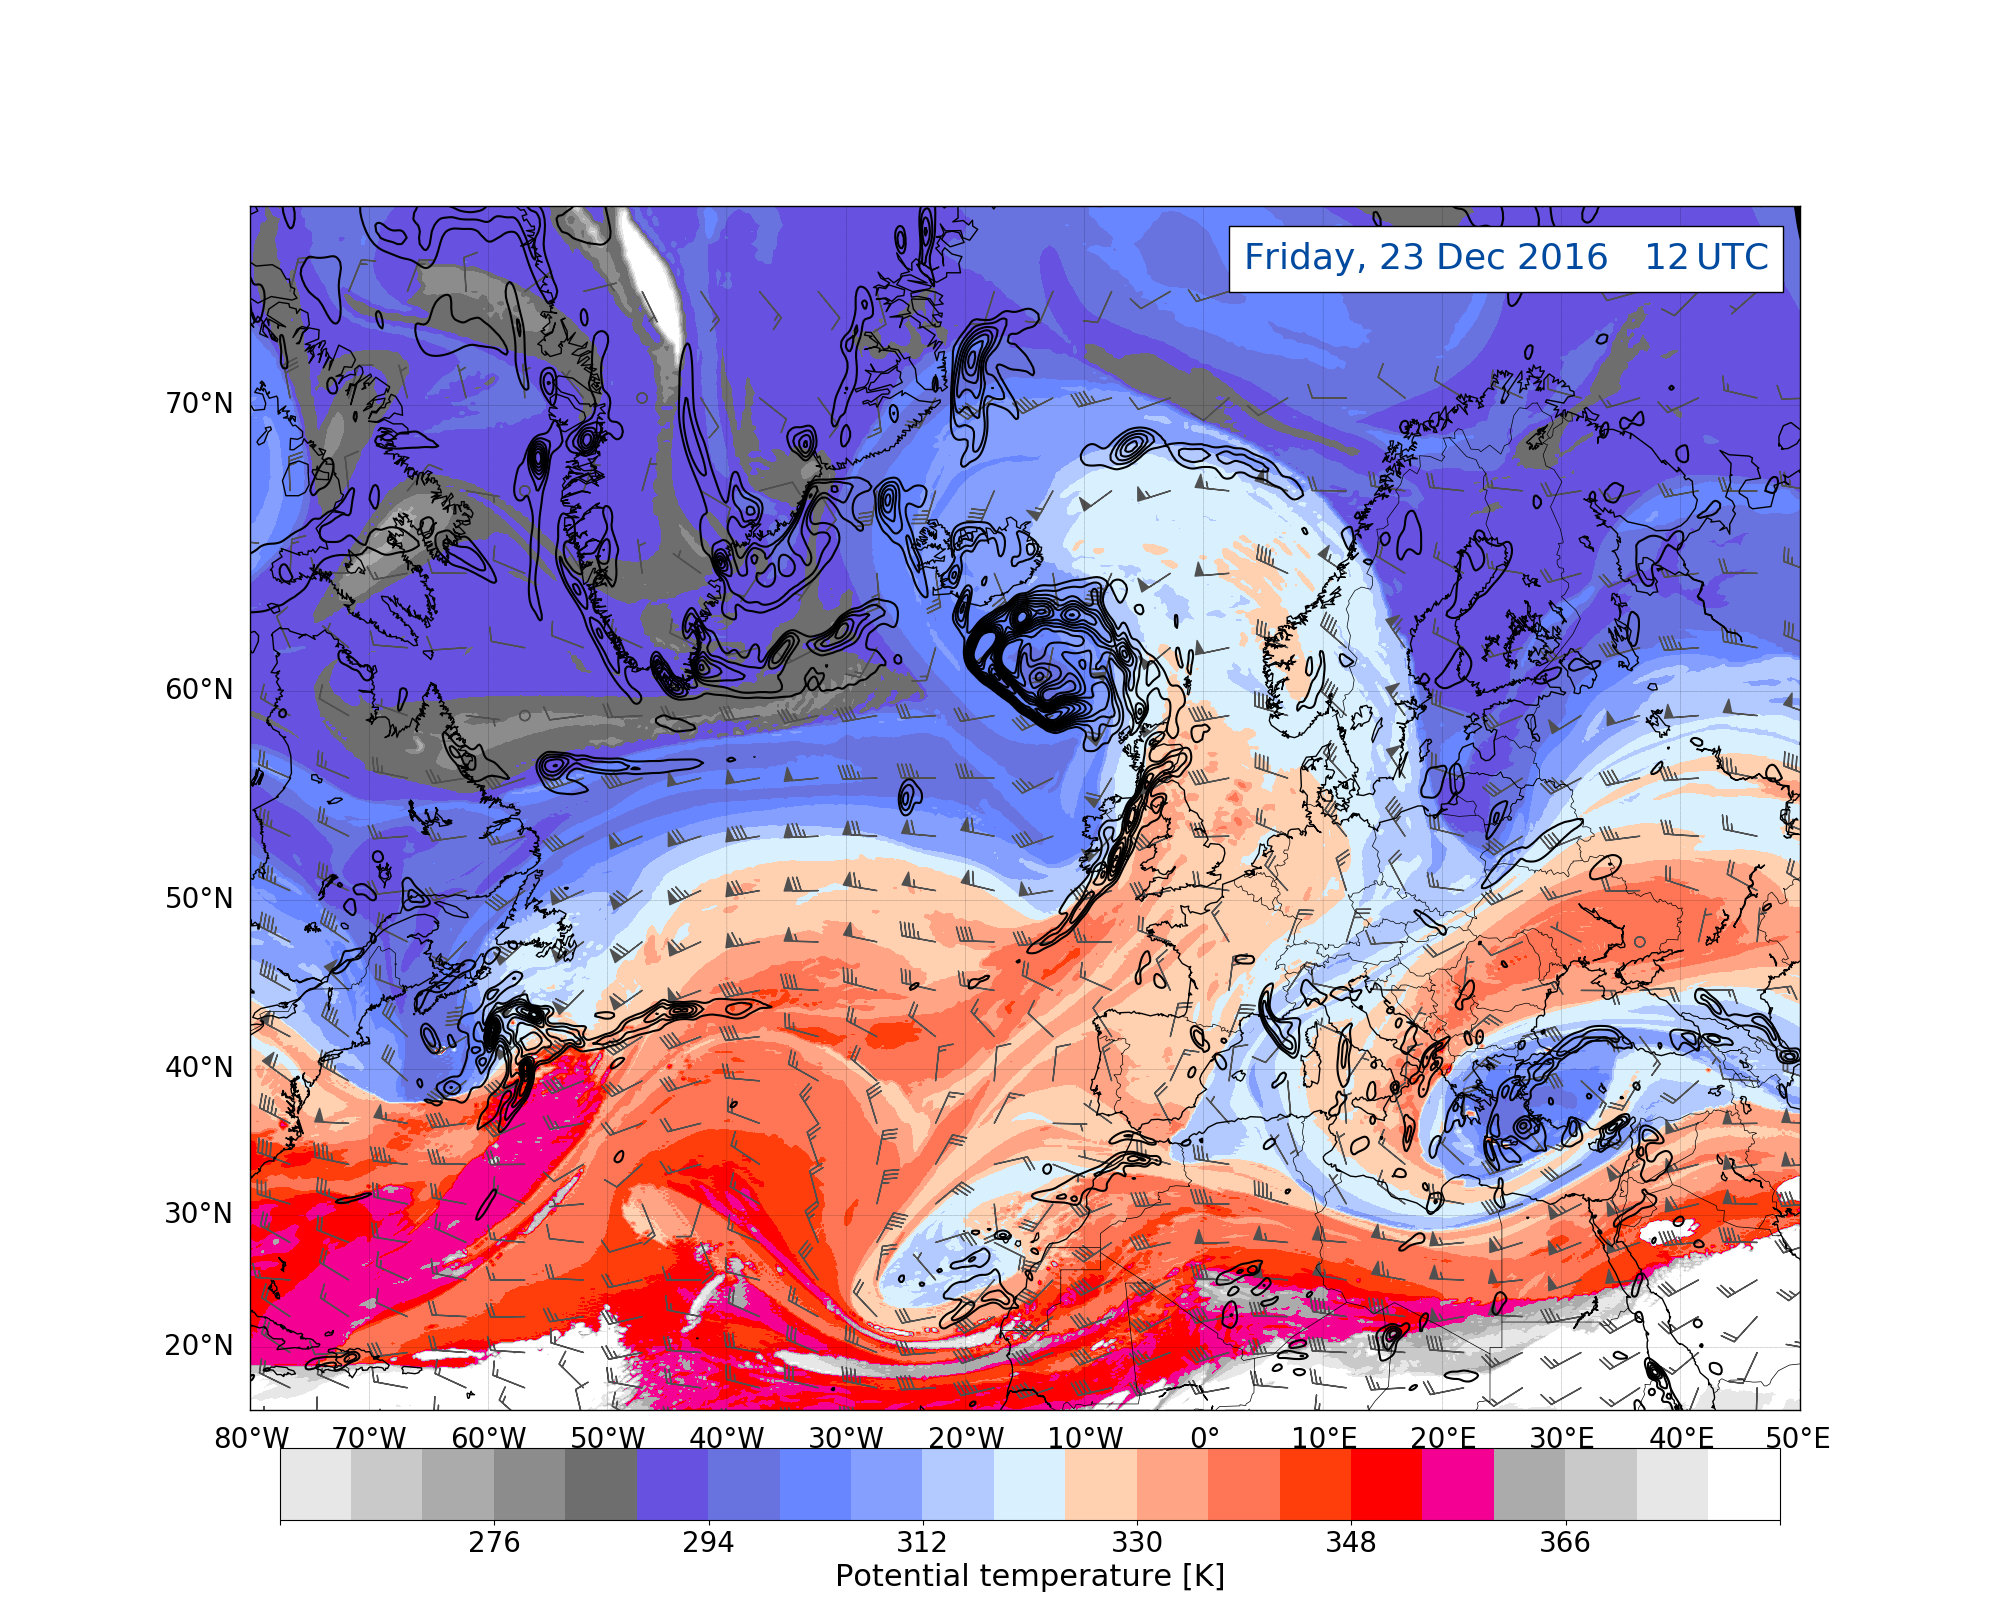
\includegraphics[trim={4.2cm 0cm 4.3cm 5.1cm},clip,
		width=\textwidth]{./fig_DynTropo/20161223_12}
		\caption{} \label{fig:DT23}
	\end{subfigure}
	\begin{subfigure}[b]{0.49\textwidth}
		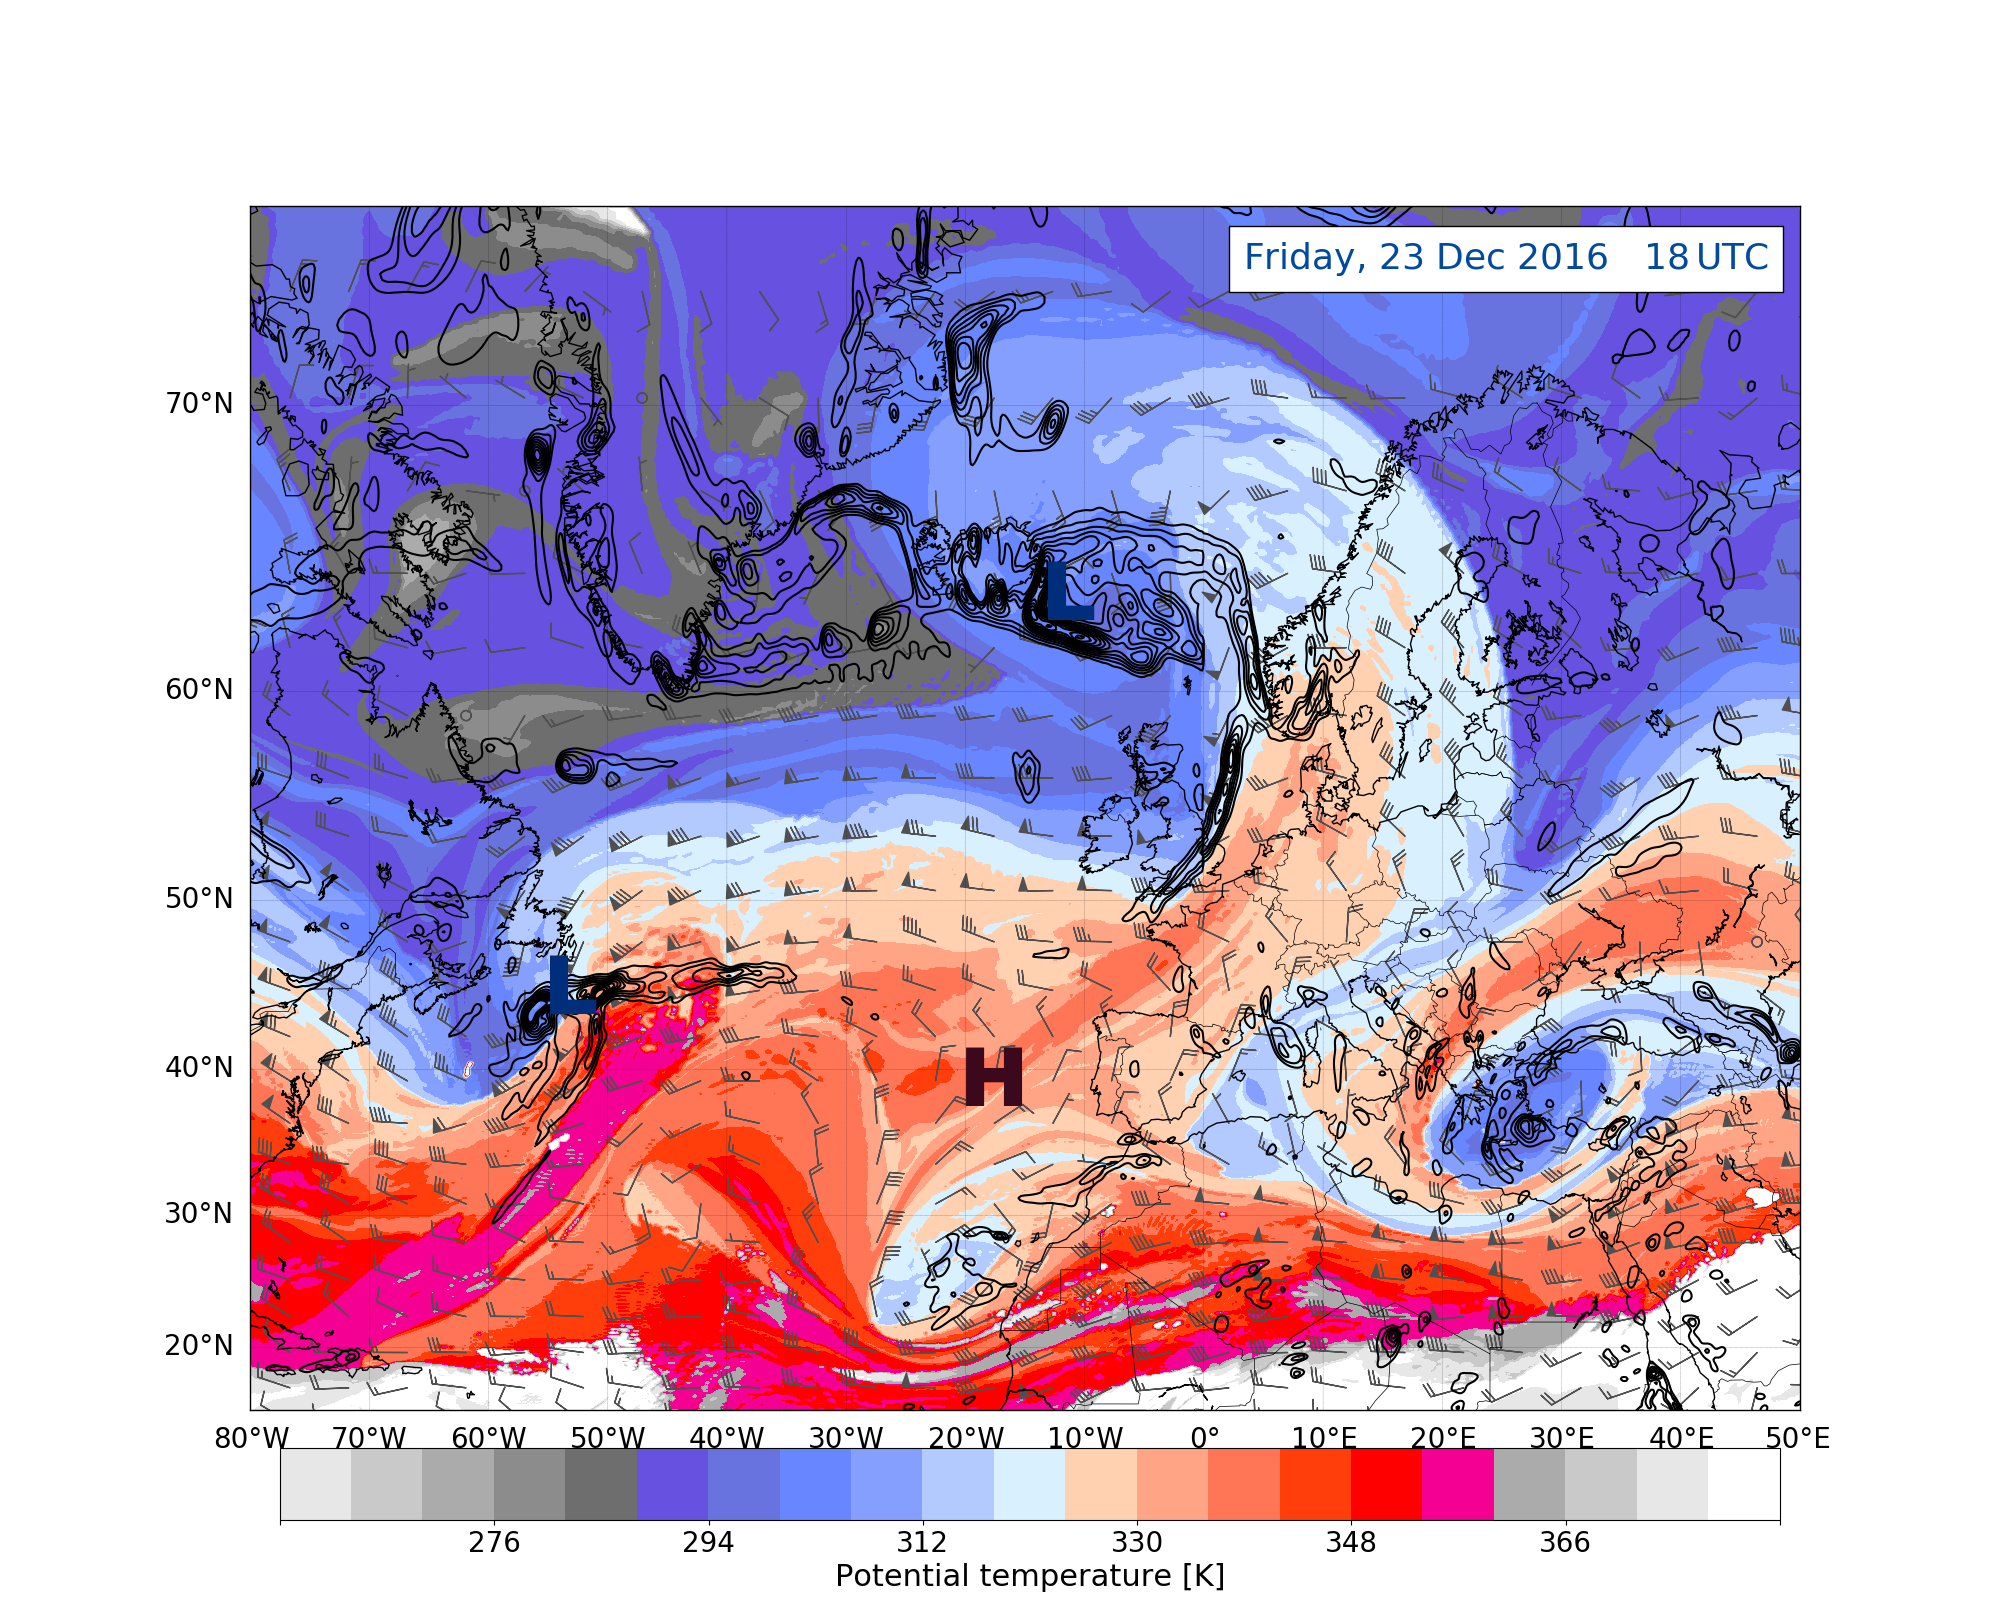
\includegraphics[trim={4.2cm 0cm 4.3cm 5.1cm},clip,
		width=\textwidth]{./fig_DynTropo/20161223_18}
		\caption{} \label{fig:DT23_18}
	\end{subfigure}
	%%% geopot %%%%
	\begin{subfigure}[b]{0.49\textwidth}
		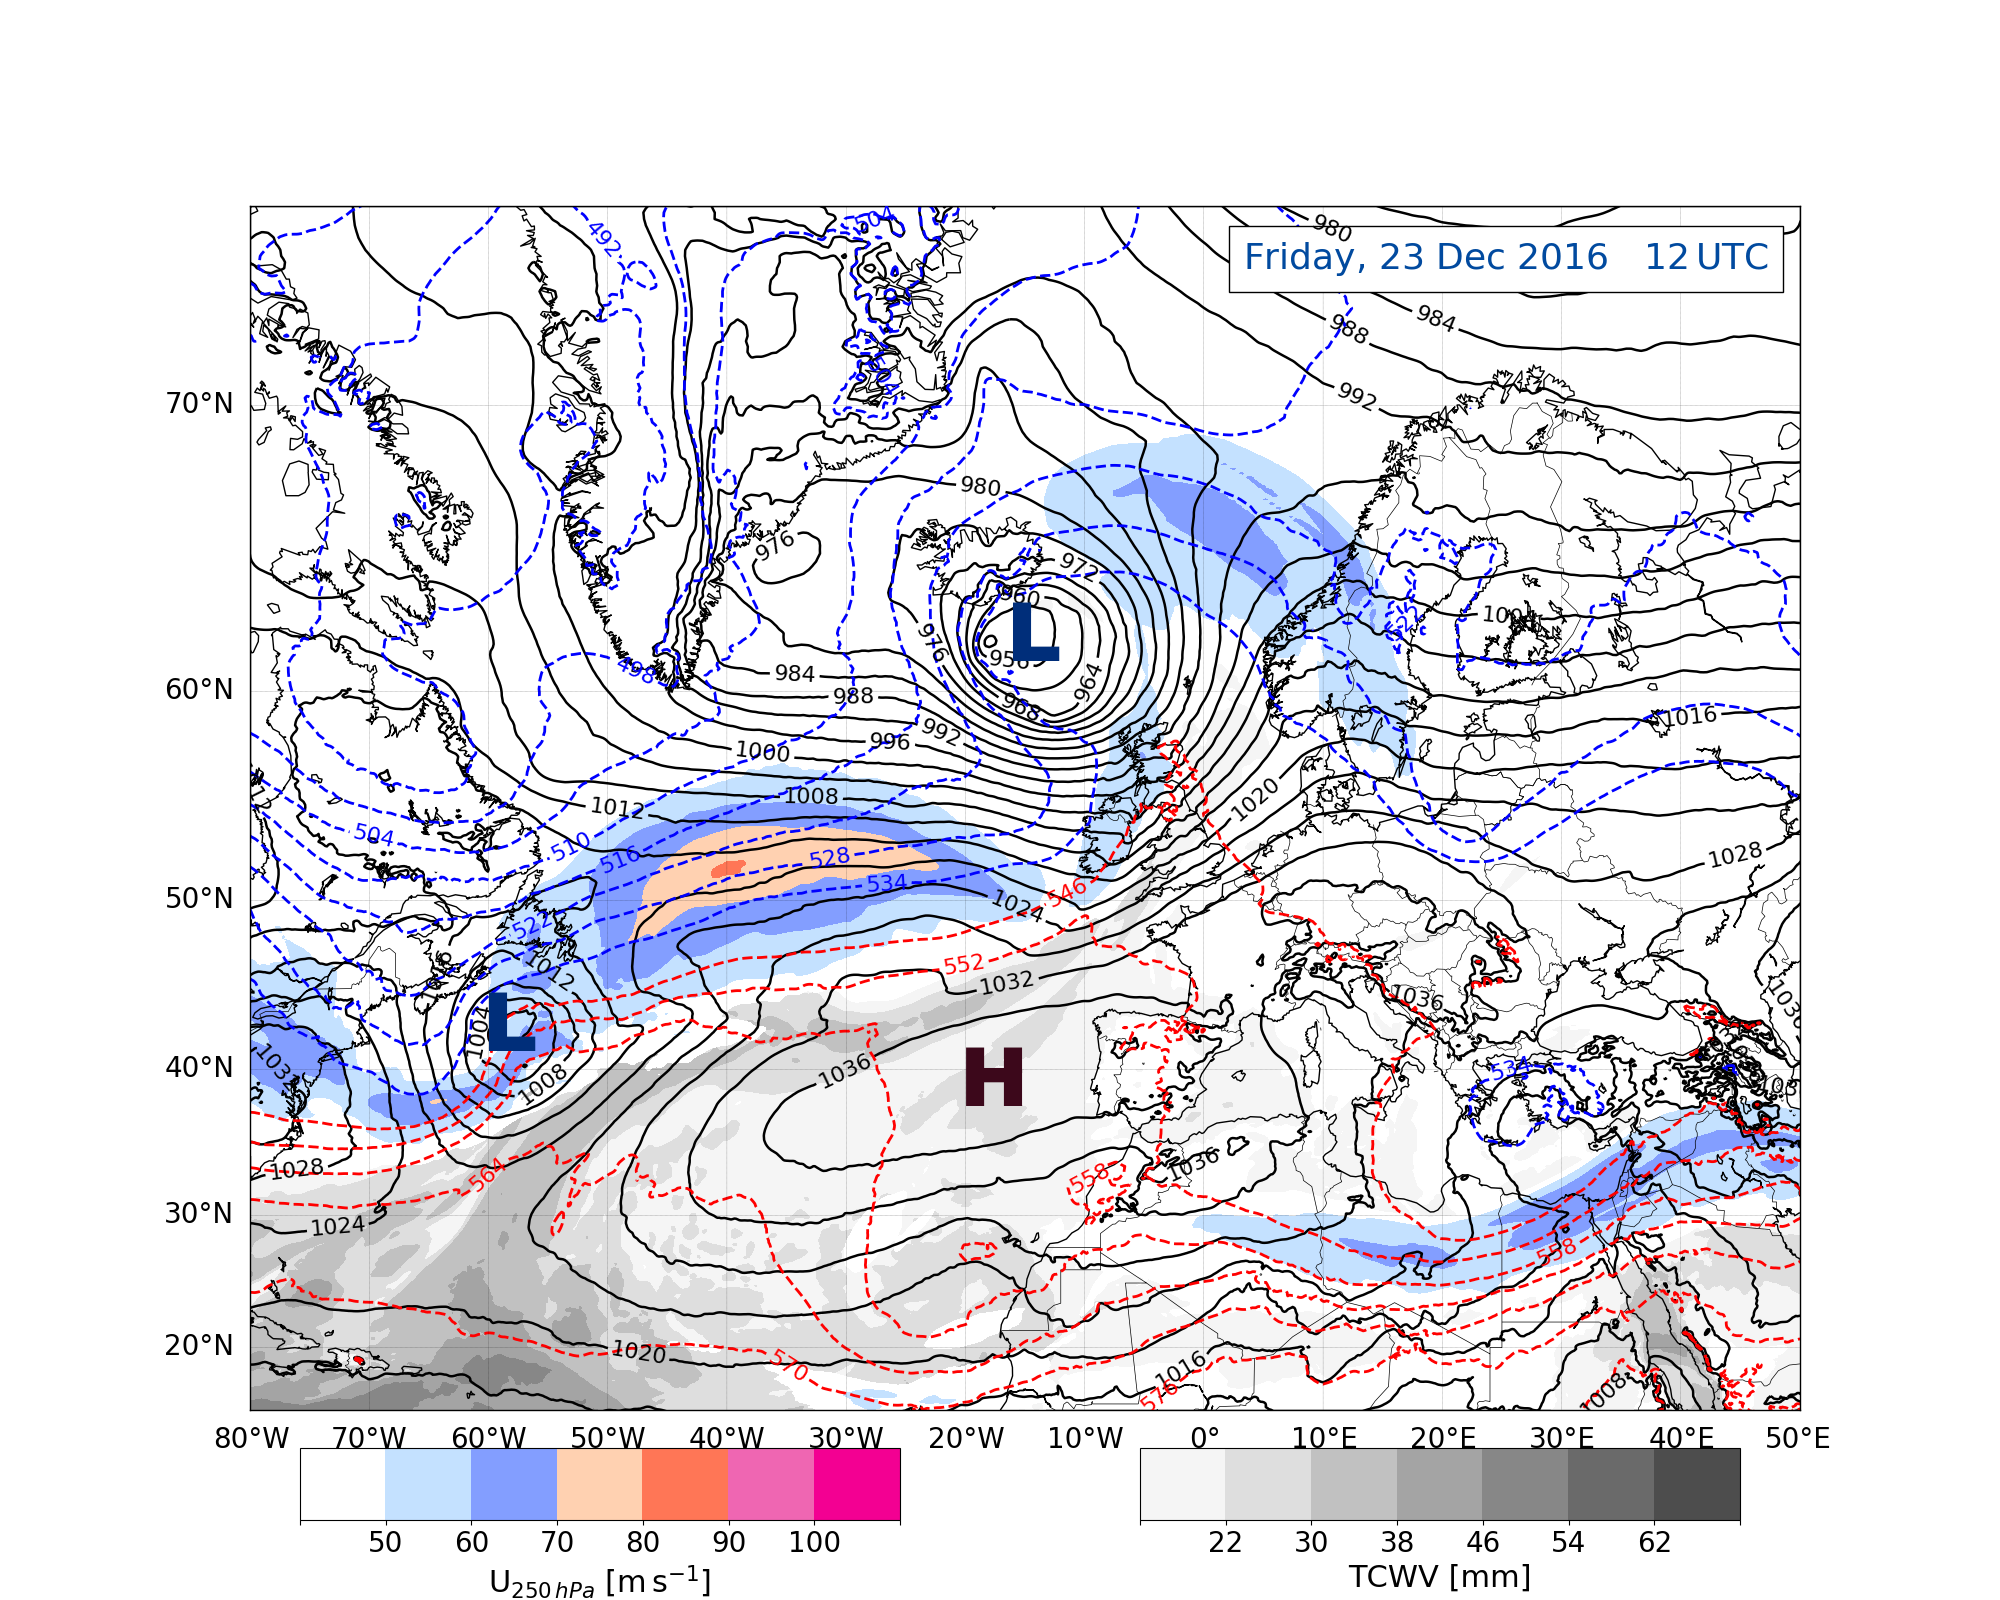
\includegraphics[trim={4.2cm 0cm 4.3cm 5.1cm},clip,
		width=\textwidth]{./fig_Geopot_Jet/20161223_12}
		\caption{} \label{fig:GP23}
	\end{subfigure}
	\begin{subfigure}[b]{0.49\textwidth}
		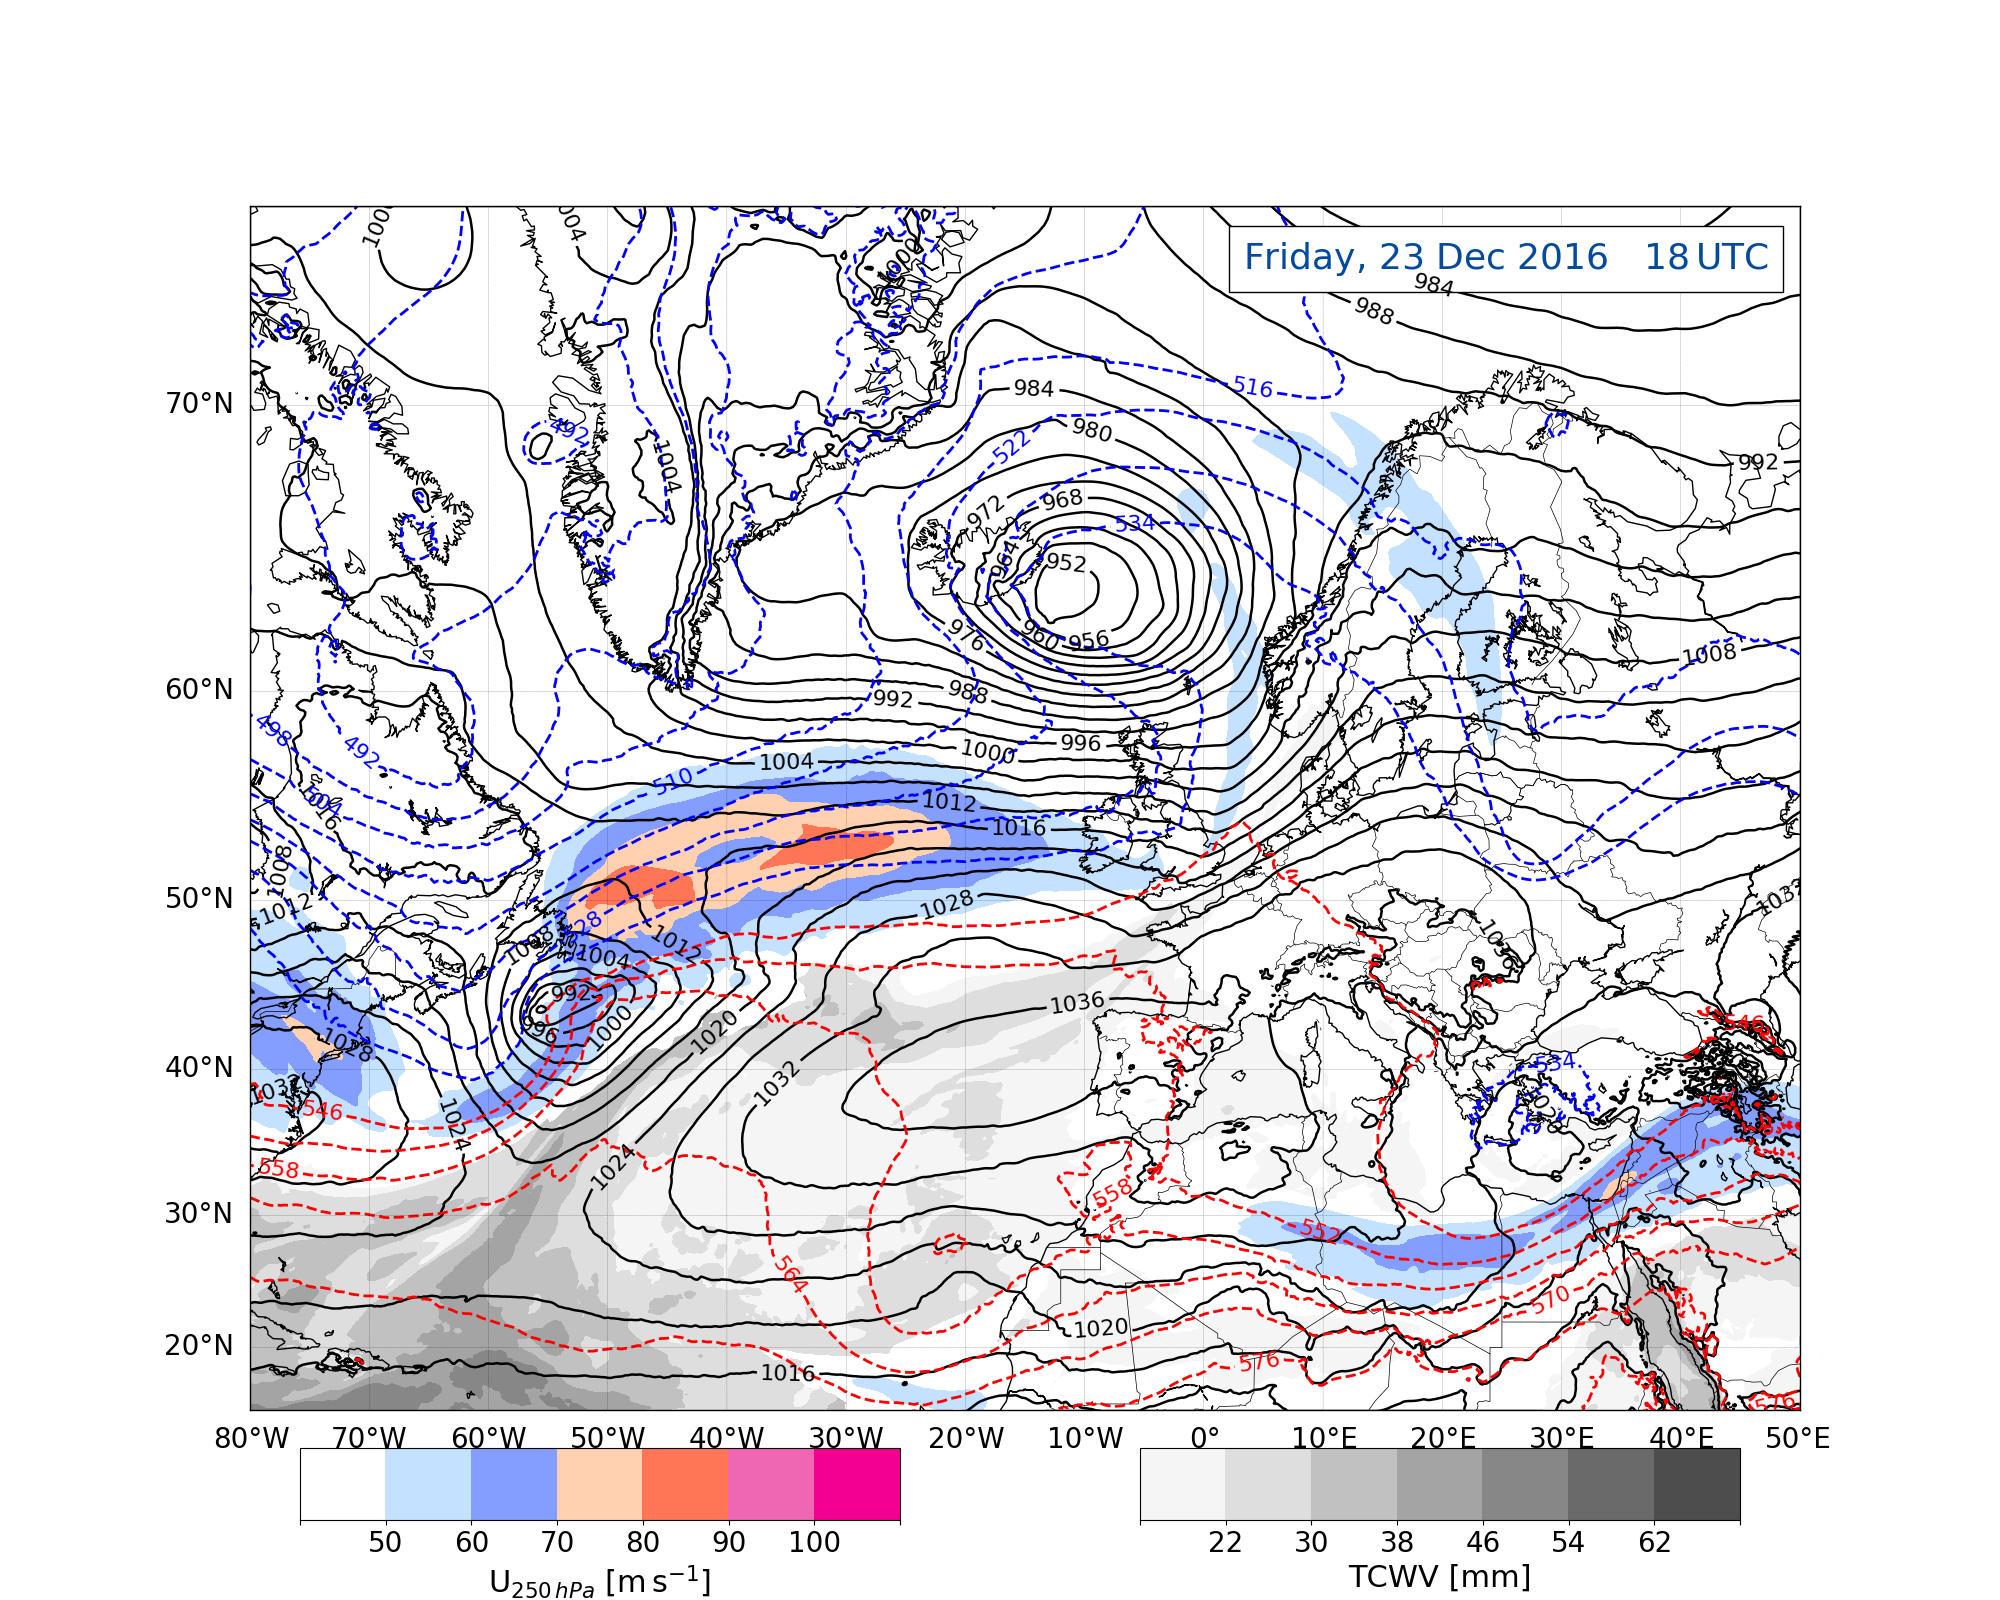
\includegraphics[trim={4.2cm 0cm 4.3cm 5.1cm},clip,
		width=\textwidth]{./fig_Geopot_Jet/20161223_18}
		\caption{} \label{fig:GP23_18}
	\end{subfigure}
	%%% local obs %%%%
	\begin{subfigure}[b]{0.49\textwidth}
		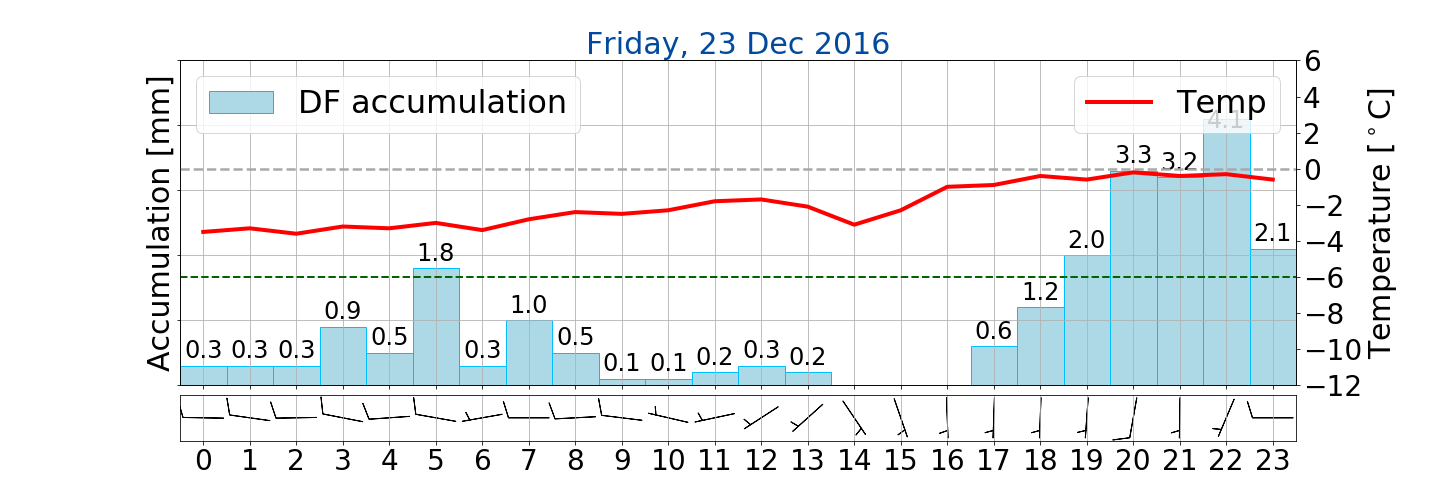
\includegraphics[trim={4.9cm 1.cm 1.5cm 1cm},clip,
		width=\textwidth]{./fig_weathermast/T_P_U_20161223}
		\caption{} \label{fig:TPU23}
	\end{subfigure}
	\caption{\textit{(As \Cref{fig:weather:19}.)} For \SI{23}{\dec} at \SI{12}{\UTC} (\protect\subref{fig:DT23}, \protect\subref{fig:GP23}) and at \SI{18}{\UTC} (\protect\subref{fig:DT23_18}, \protect\subref{fig:GP23_18}).}\label{fig:weather:23}
\end{figure}
%%%%%%%%%%%%%%%%%%%%%%%%%%%%%%%%%%%%%%%%%%%%%%%%%%%%%%%%%%%%%%


\newpage
\subsection*{\SI{24}{\dec}}
%%% 24/12
% 24/00
% Norway goes right back into colder air @ DT, @ sfc (thickness lines)
% @ DT lifting associated with the low-level vorticity 
% 24/12
% Cold frontal boundary pushes through
% Norway is back into colder air → reduction in temp.
% Again, westerly flow → good for orographic lifting
After the passage of the occluded front over Norway, passes cold air into Scandinavia (\Cref{fig:DT24}, \subref{fig:GP24}).
The temperature drops in \Cref{fig:TPU24}), and solid phase precipitation resumes. The importance of moisture transport is emphasized by the integrated water vapour plot (\Cref{fig:AR24}). This represents a crucial component to the high precipitation amounts that were measured at the observational site. This represents a quantitative confirmation of previous climatological studies of extreme, cold-season precipitation \citep[][unpublished]{azad_extreme_2017,moore_large_2018}. 
%%%%%%%%%%%%%%%%%%%%%%%%%%%%%%%%%%%%%%%%%%%%%%%%%%%%%%%%%%%%%%
\begin{figure}[ht!]%\ContinuedFloat
	\centering
	%%% dyntropo %%%%
	\begin{subfigure}[b]{0.49\textwidth}
		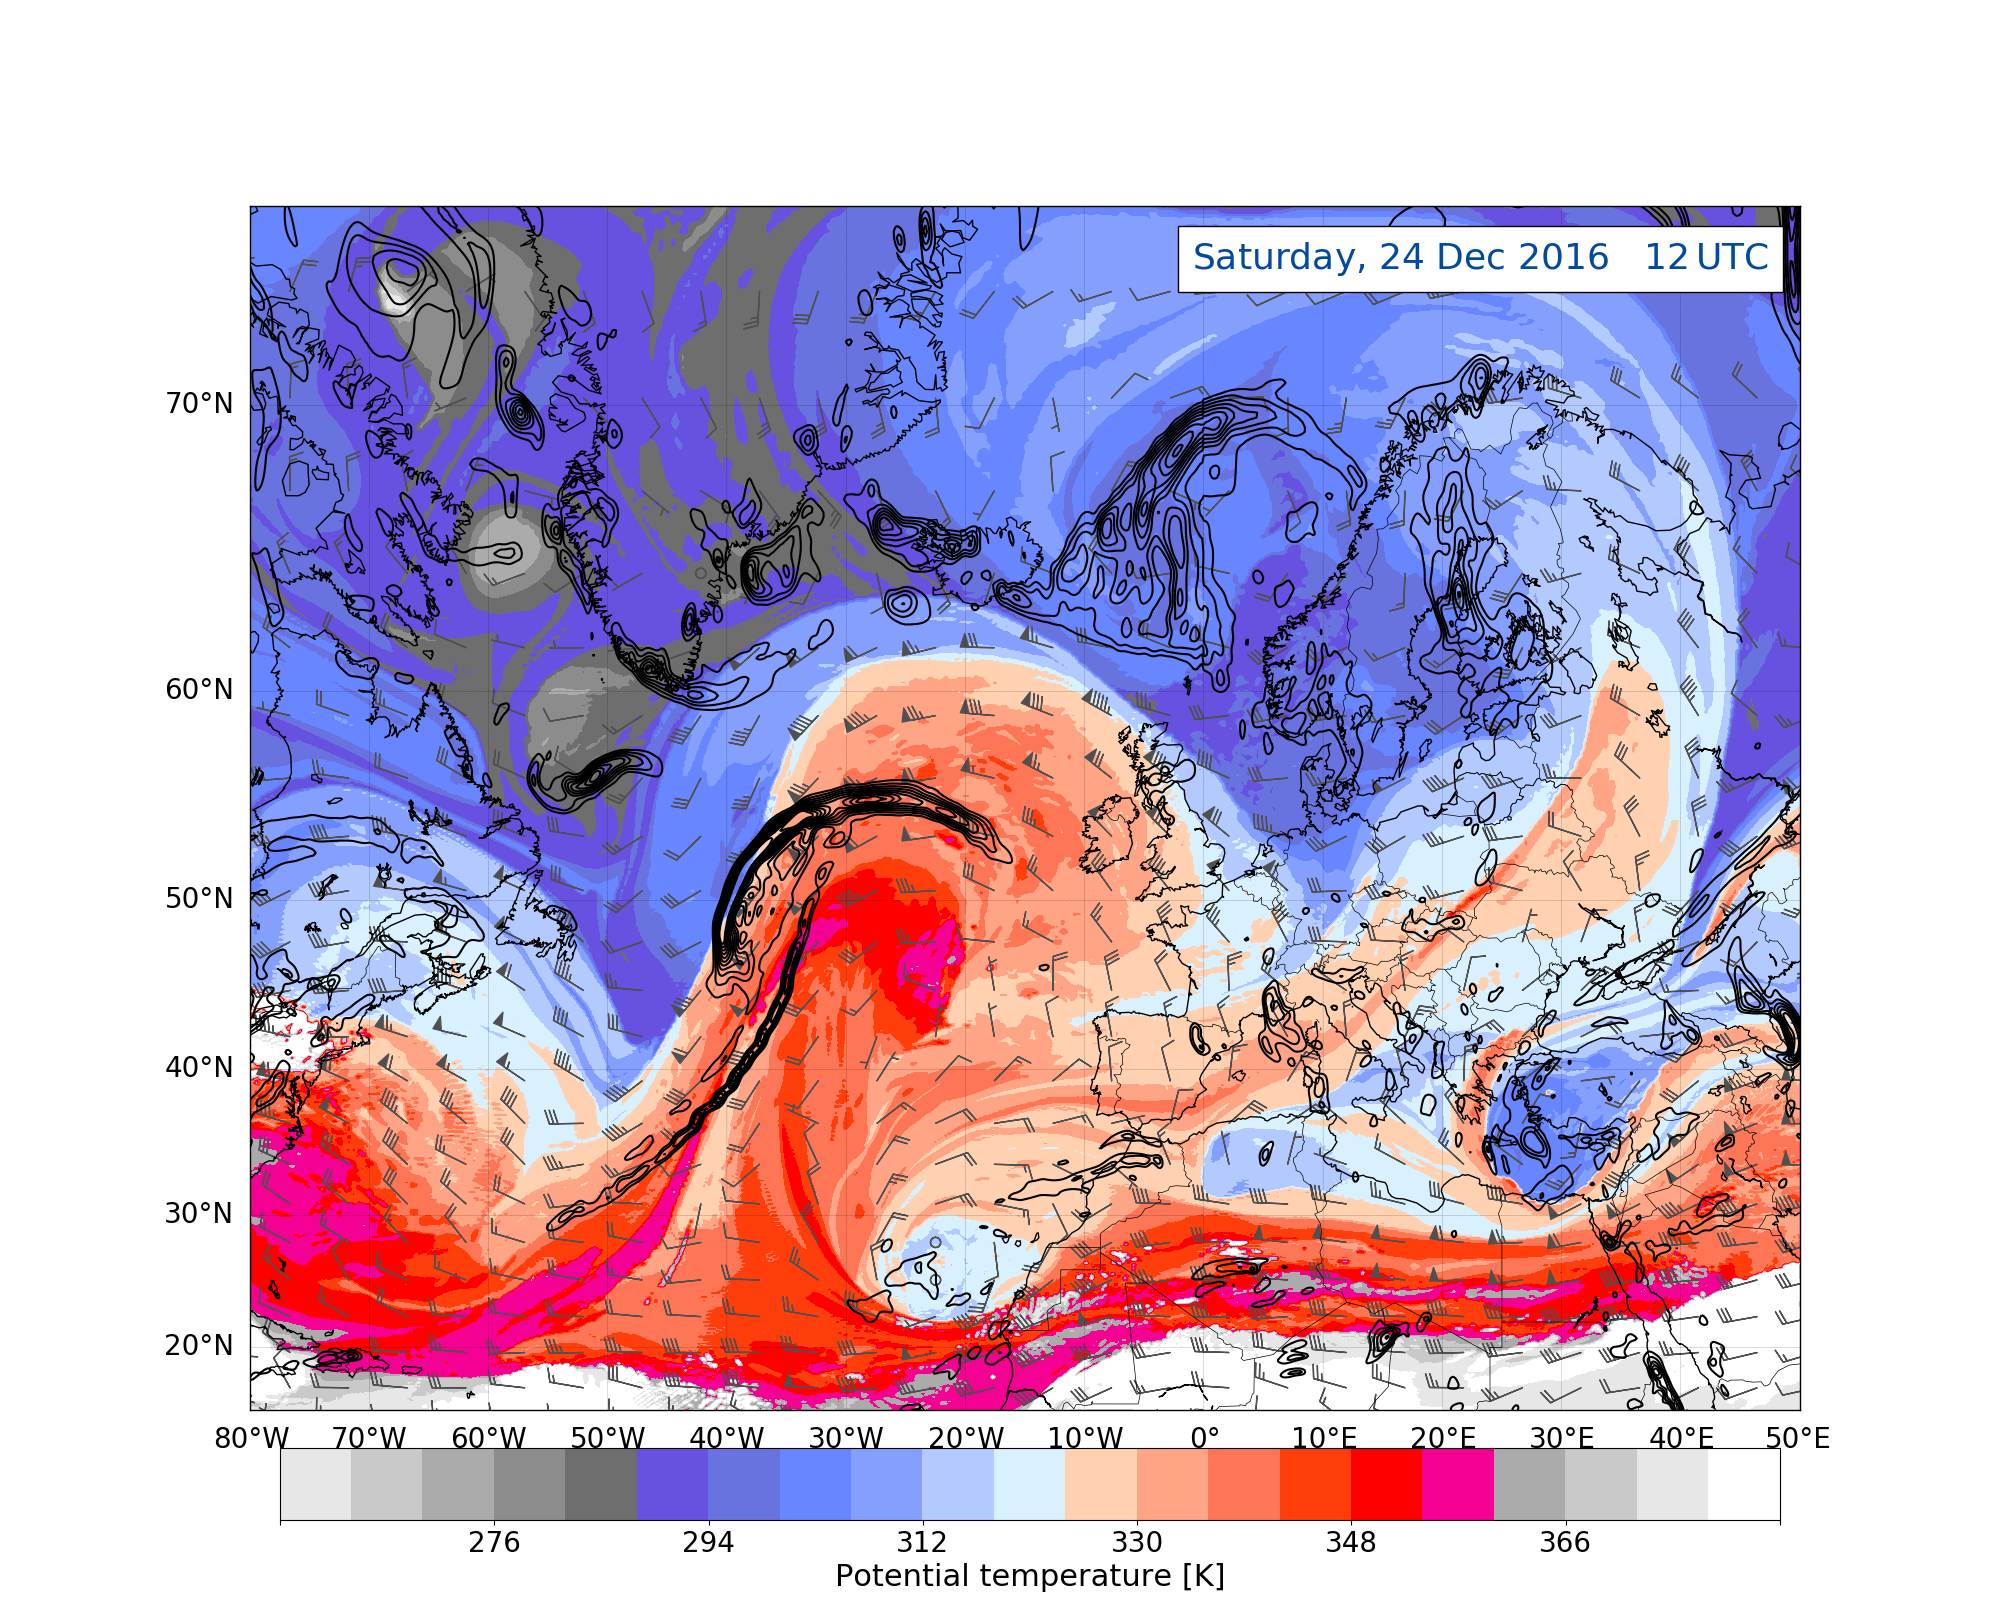
\includegraphics[trim={4.2cm 0cm 4.3cm 5.1cm},clip,
		width=\textwidth]{./fig_DynTropo/20161224_12}
		\caption{} \label{fig:DT24}
	\end{subfigure}
	%%% geopot %%%%
	\begin{subfigure}[b]{0.49\textwidth}
		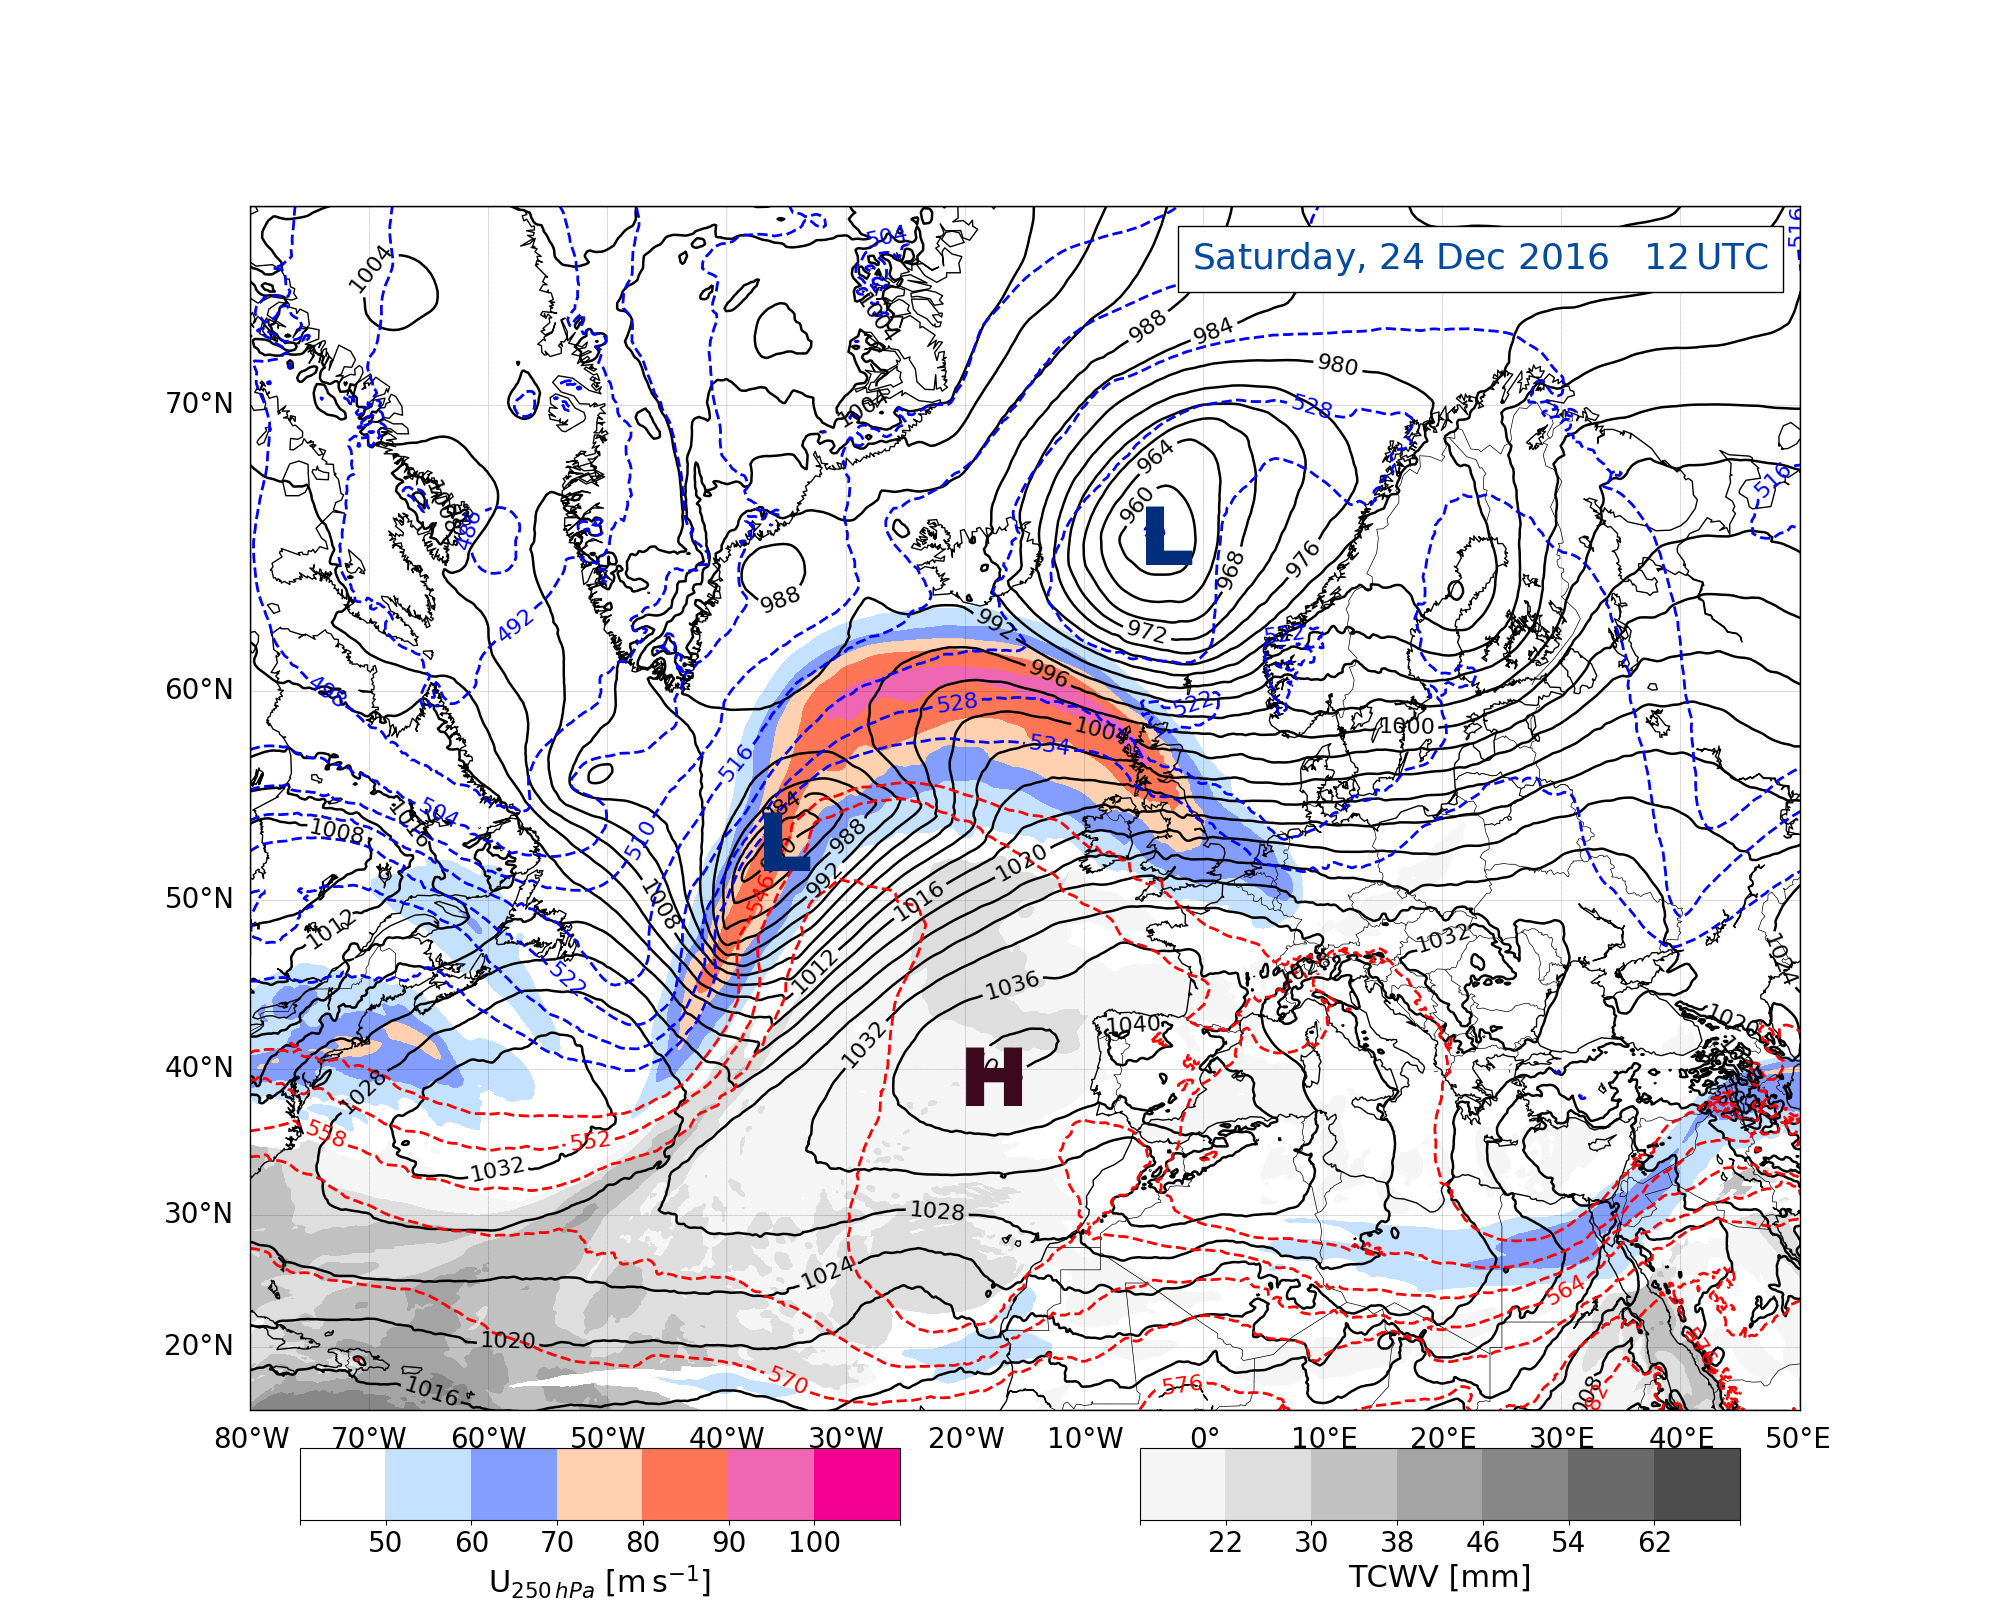
\includegraphics[trim={4.2cm 0cm 4.3cm 5.1cm},clip,
		width=\textwidth]{./fig_Geopot_Jet/20161224_12}
		\caption{} \label{fig:GP24}
	\end{subfigure}
	%%% local obs %%%%
	\begin{subfigure}[b]{0.49\textwidth}
		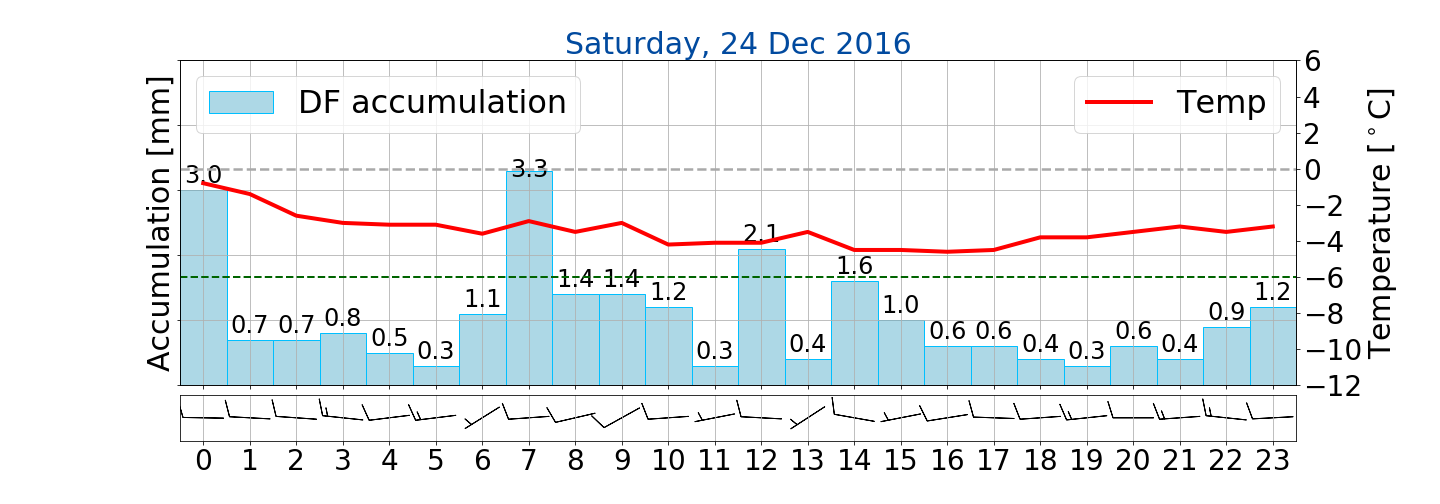
\includegraphics[trim={4.9cm 1.cm 1.5cm 1cm},clip,
		width=\textwidth]{./fig_weathermast/T_P_U_20161224}
		\caption{} \label{fig:TPU24}
	\end{subfigure}
	\caption{\textit{(As \Cref{fig:weather:19}.)} For \SI{24}{\dec} at \SI{12}{\UTC}.}\label{fig:weather:24}
\end{figure}
%%%%%%%%%%%%%%%%%%%%%%%%%%%%%%%%%%%%%%%%%%%%%%%%%%%%%%%%%%%%%%

\newpage
\subsection*{\SI{25}{\dec}}
%%% 25/12
% 25/00
% @ DT ridging coming in
% @ sfc, low with frontal boundaries
% Jet exit region is directly over Norway → Haukeliseter on right exit region? → sinking?
% Some orographic lifting
% 25/12
% Warm front comes through
% → low-level vorticity → orographic lifting
% 25/18
% Ridging bring more warm air to Norway (should be moist too → check total water vapor)
% Norway in warm sector
% Conducive westerly flow → orographic lifting
Twenty-four hours later the upper level ridge is more pronounced and covers large parts of Norway (\Cref{fig:DT25}. The cyclone south-east of Iceland has built its frontal boundaries (\Cref{fig:GP25}). Between \SIlist{12;18}{\UTC} the warm sector passes through Haukeliseter (\Cref{fig:GP25}, \subref{fig:GP25_18}, \subref{fig:TPU25}). Connected to the warm sector the temperature rises in \Cref{fig:TPU25} and the precipitation becomes liquid. 
%%%%%%%%%%%%%%%%%%%%%%%%%%%%%%%%%%%%%%%%%%%%%%%%%%%%%%%%%%%%%%
\begin{figure}[ht!]%\ContinuedFloat
	\centering
	%%% dyntropo %%%%
	\begin{subfigure}[b]{0.49\textwidth}
		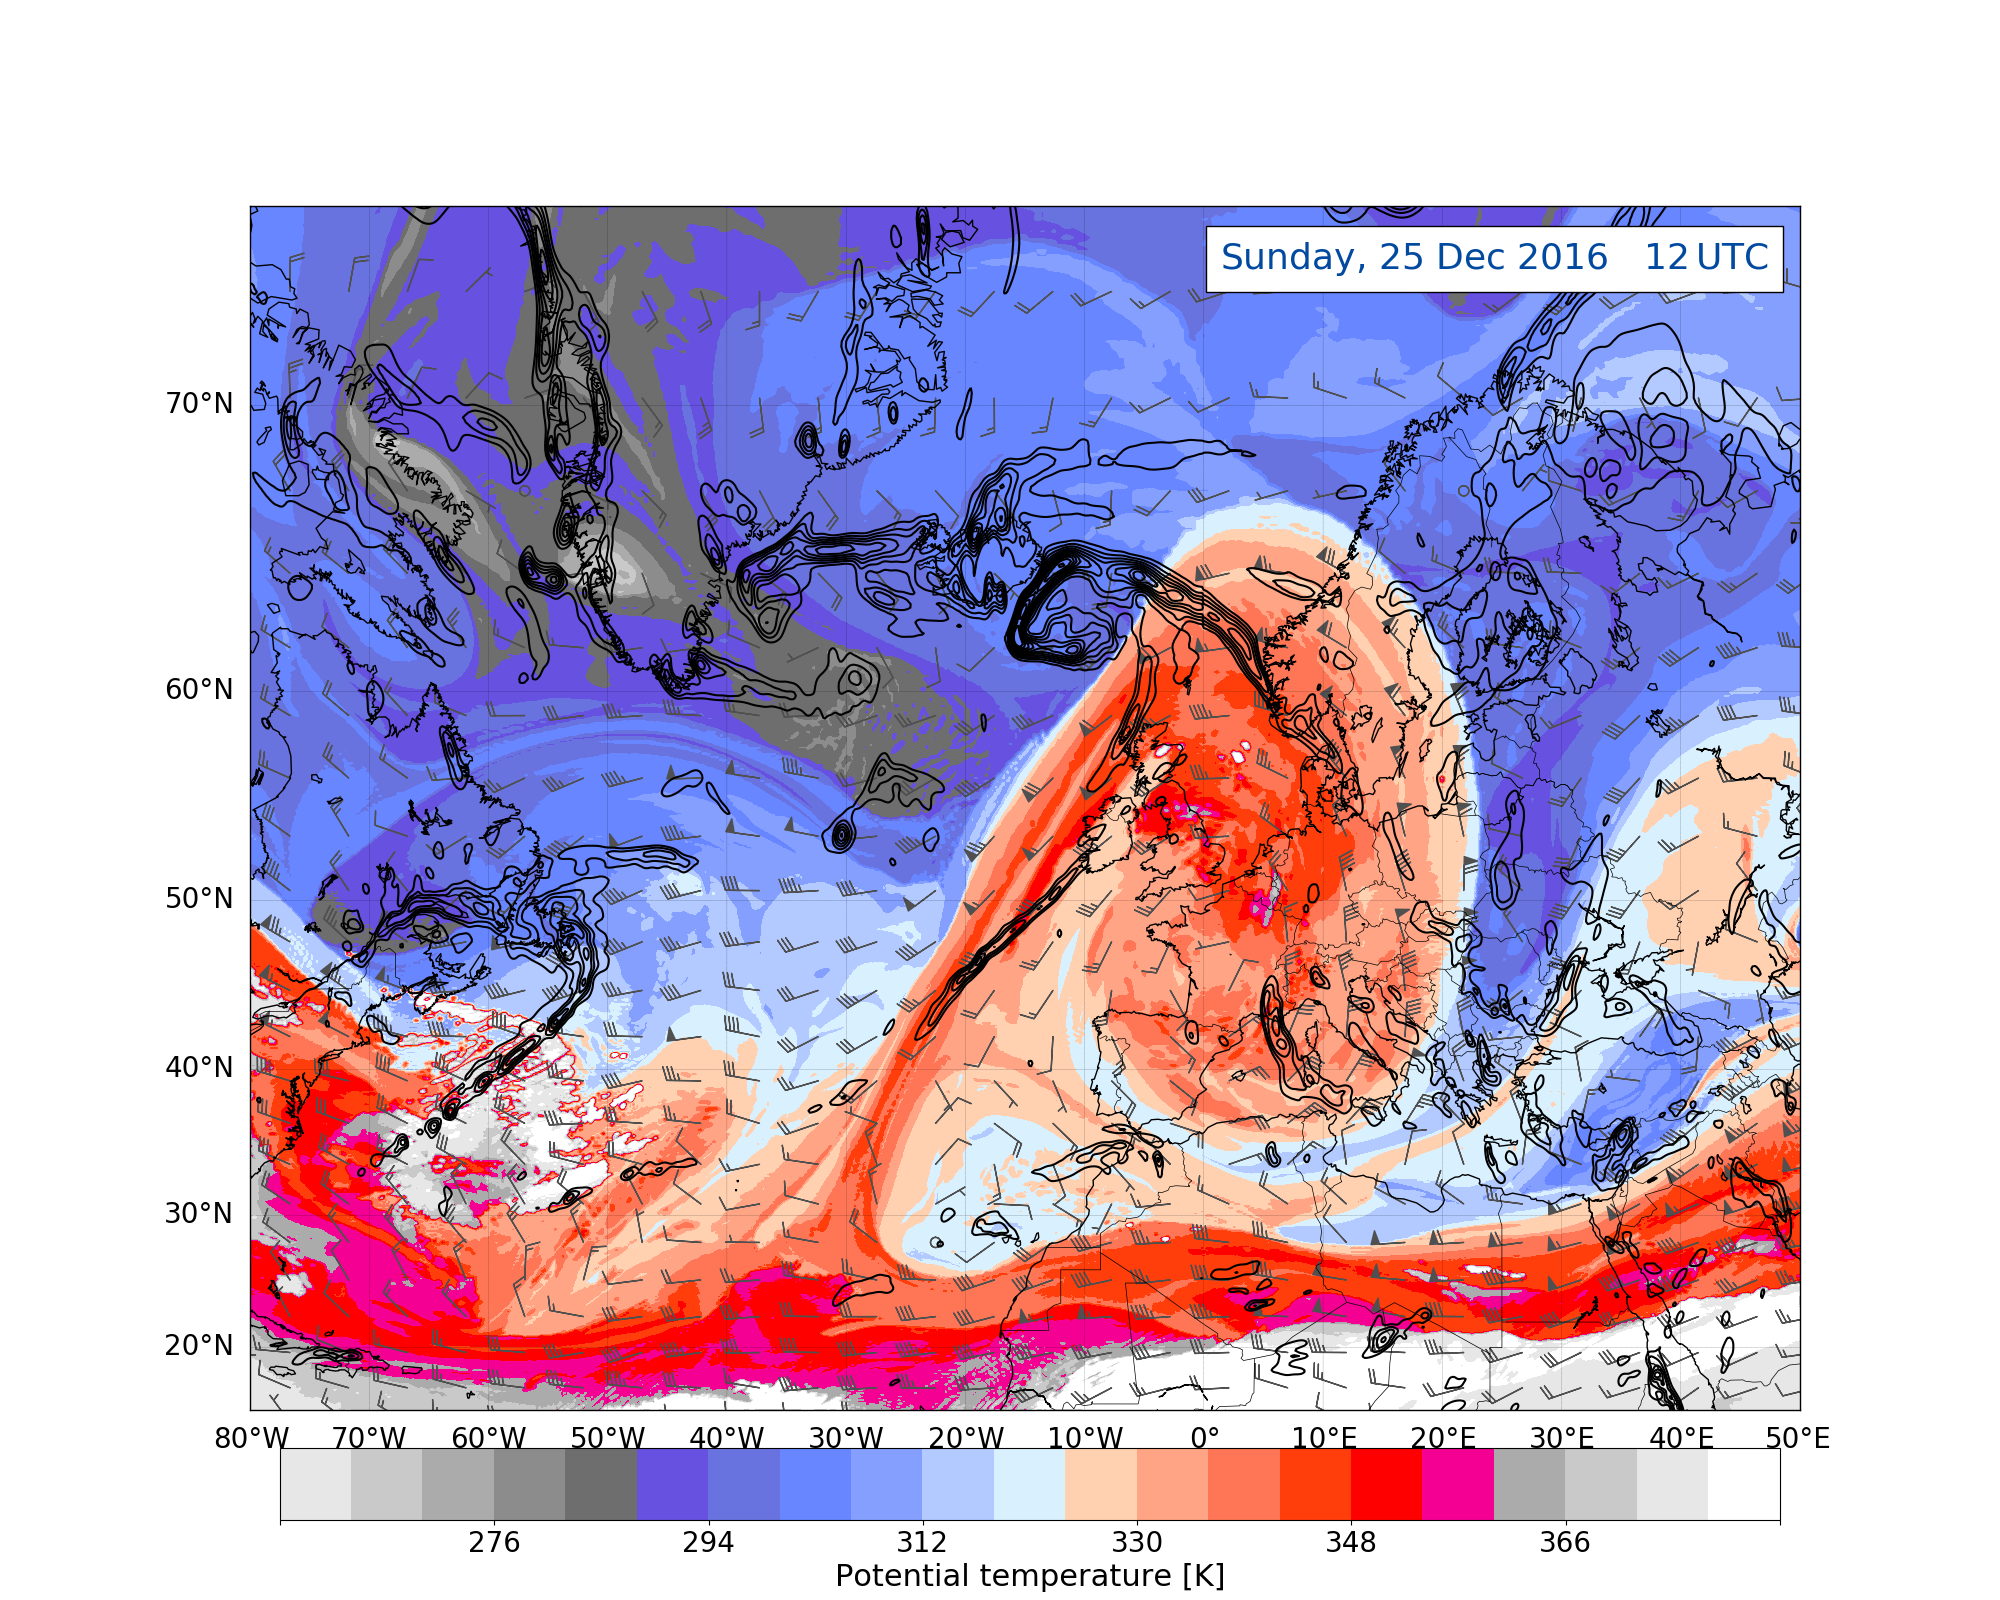
\includegraphics[trim={4.2cm 0cm 4.3cm 5.1cm},clip,
		width=\textwidth]{./fig_DynTropo/20161225_12}
		\caption{} \label{fig:DT25}
	\end{subfigure}
	\begin{subfigure}[b]{0.49\textwidth}
		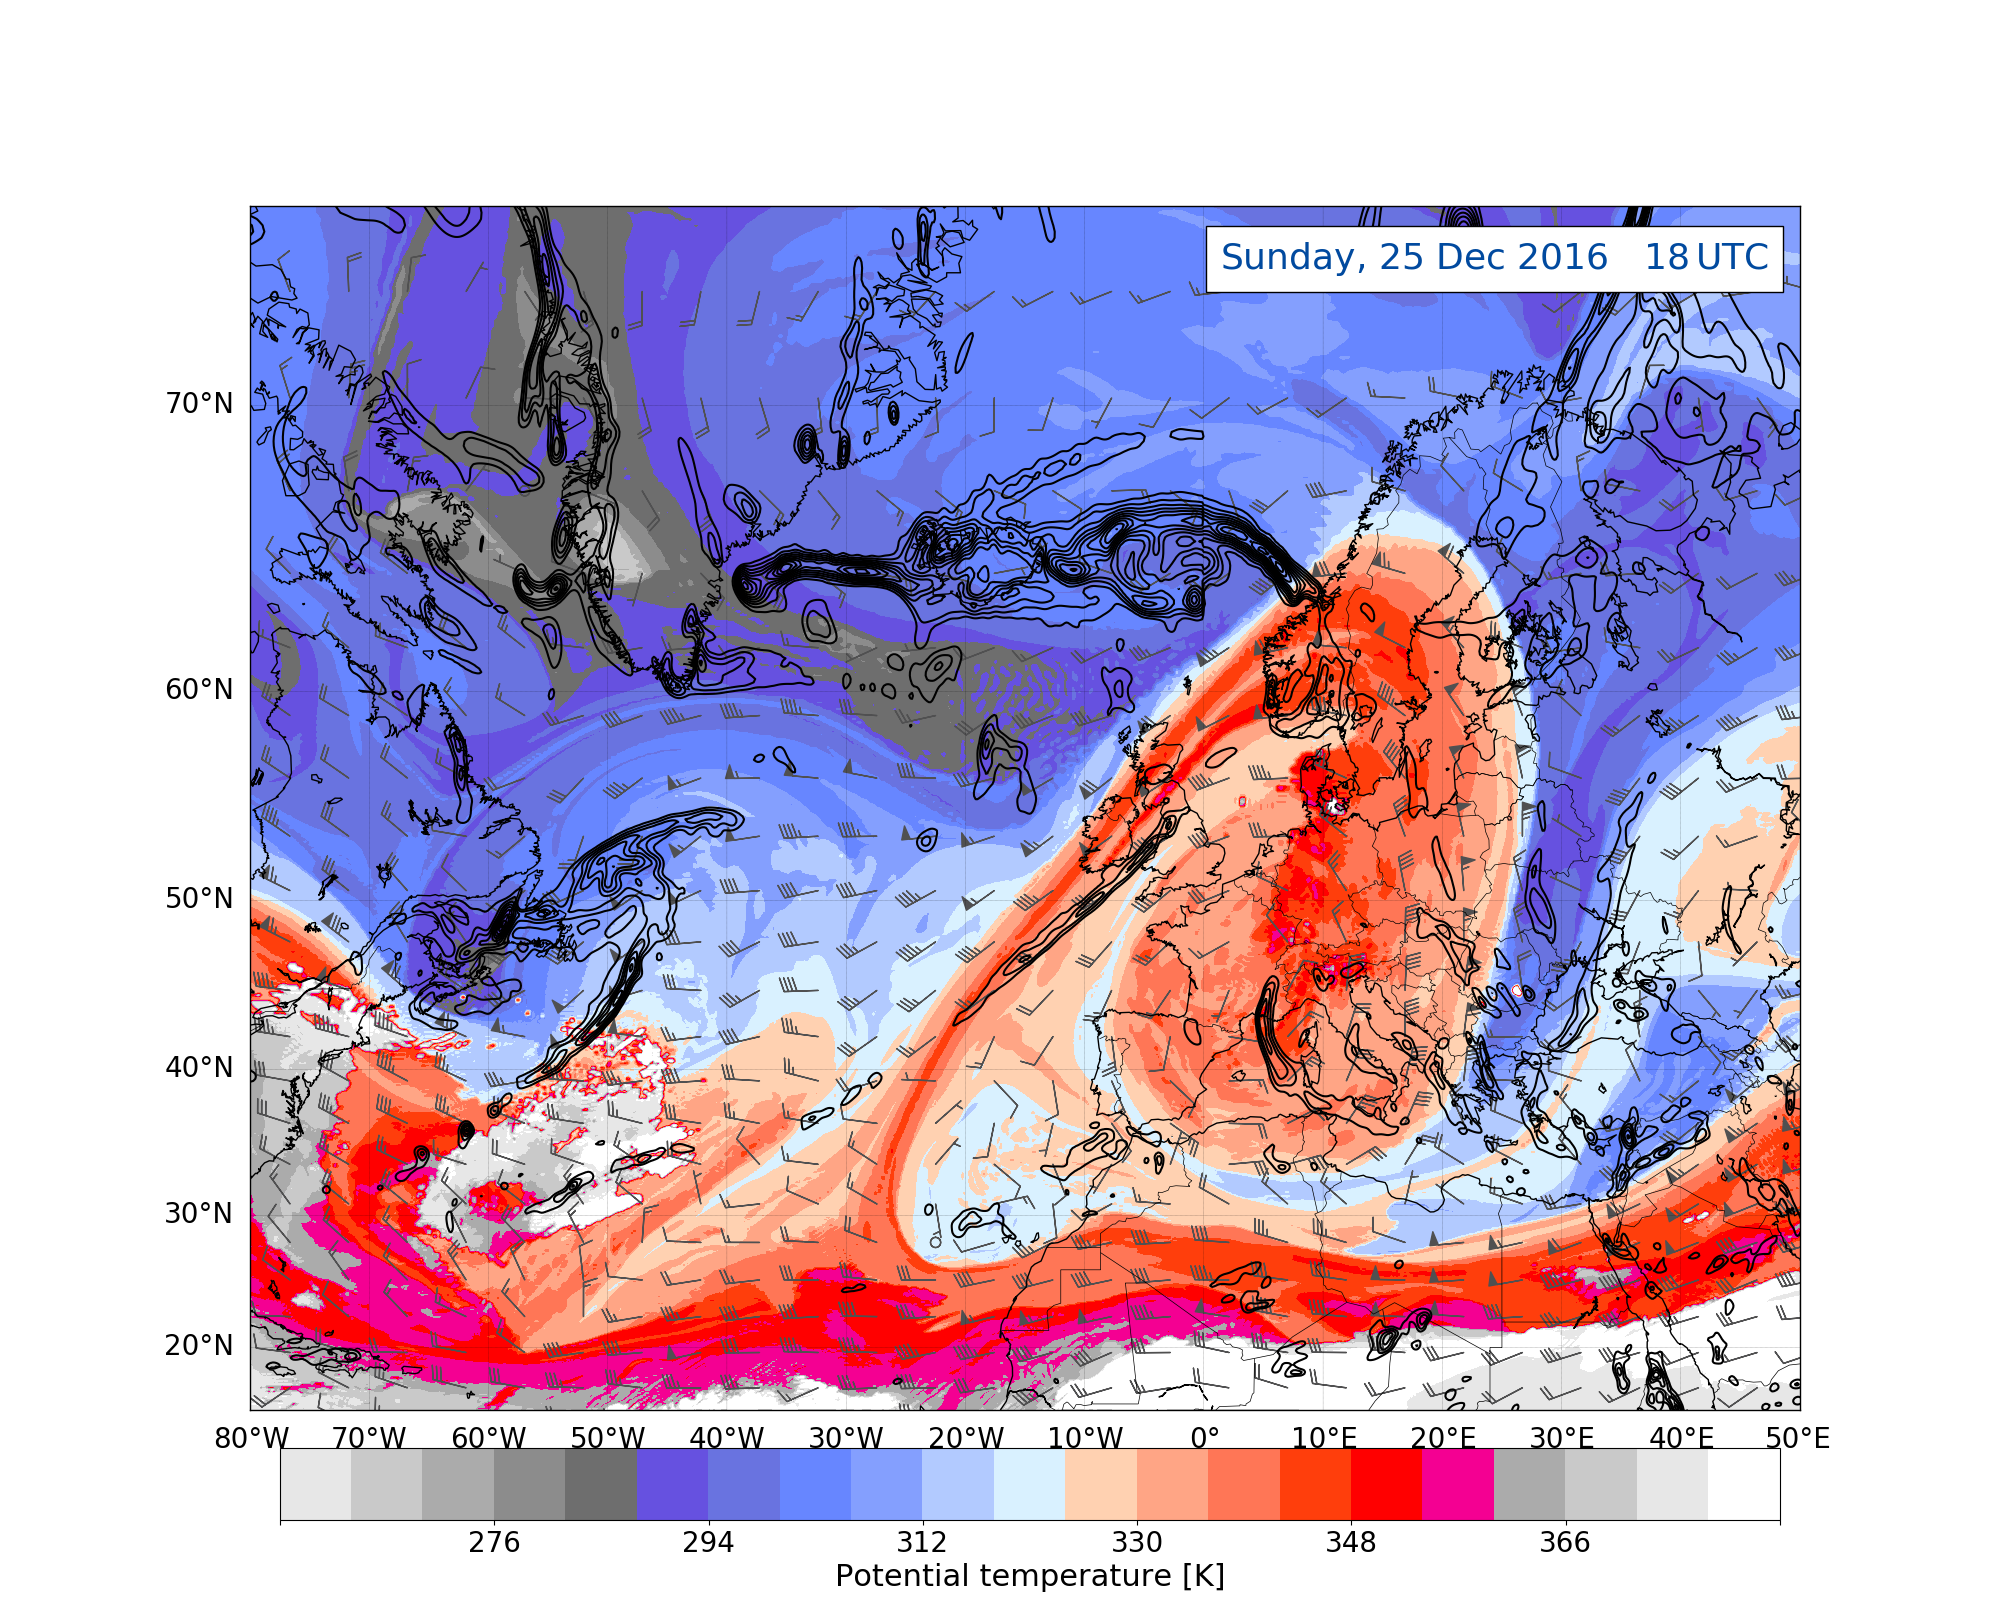
\includegraphics[trim={4.2cm 0cm 4.3cm 5.1cm},clip,
		width=\textwidth]{./fig_DynTropo/20161225_18}
		\caption{} \label{fig:DT25_18}
	\end{subfigure}
	%%% geopot %%%%
	\begin{subfigure}[b]{0.49\textwidth}
		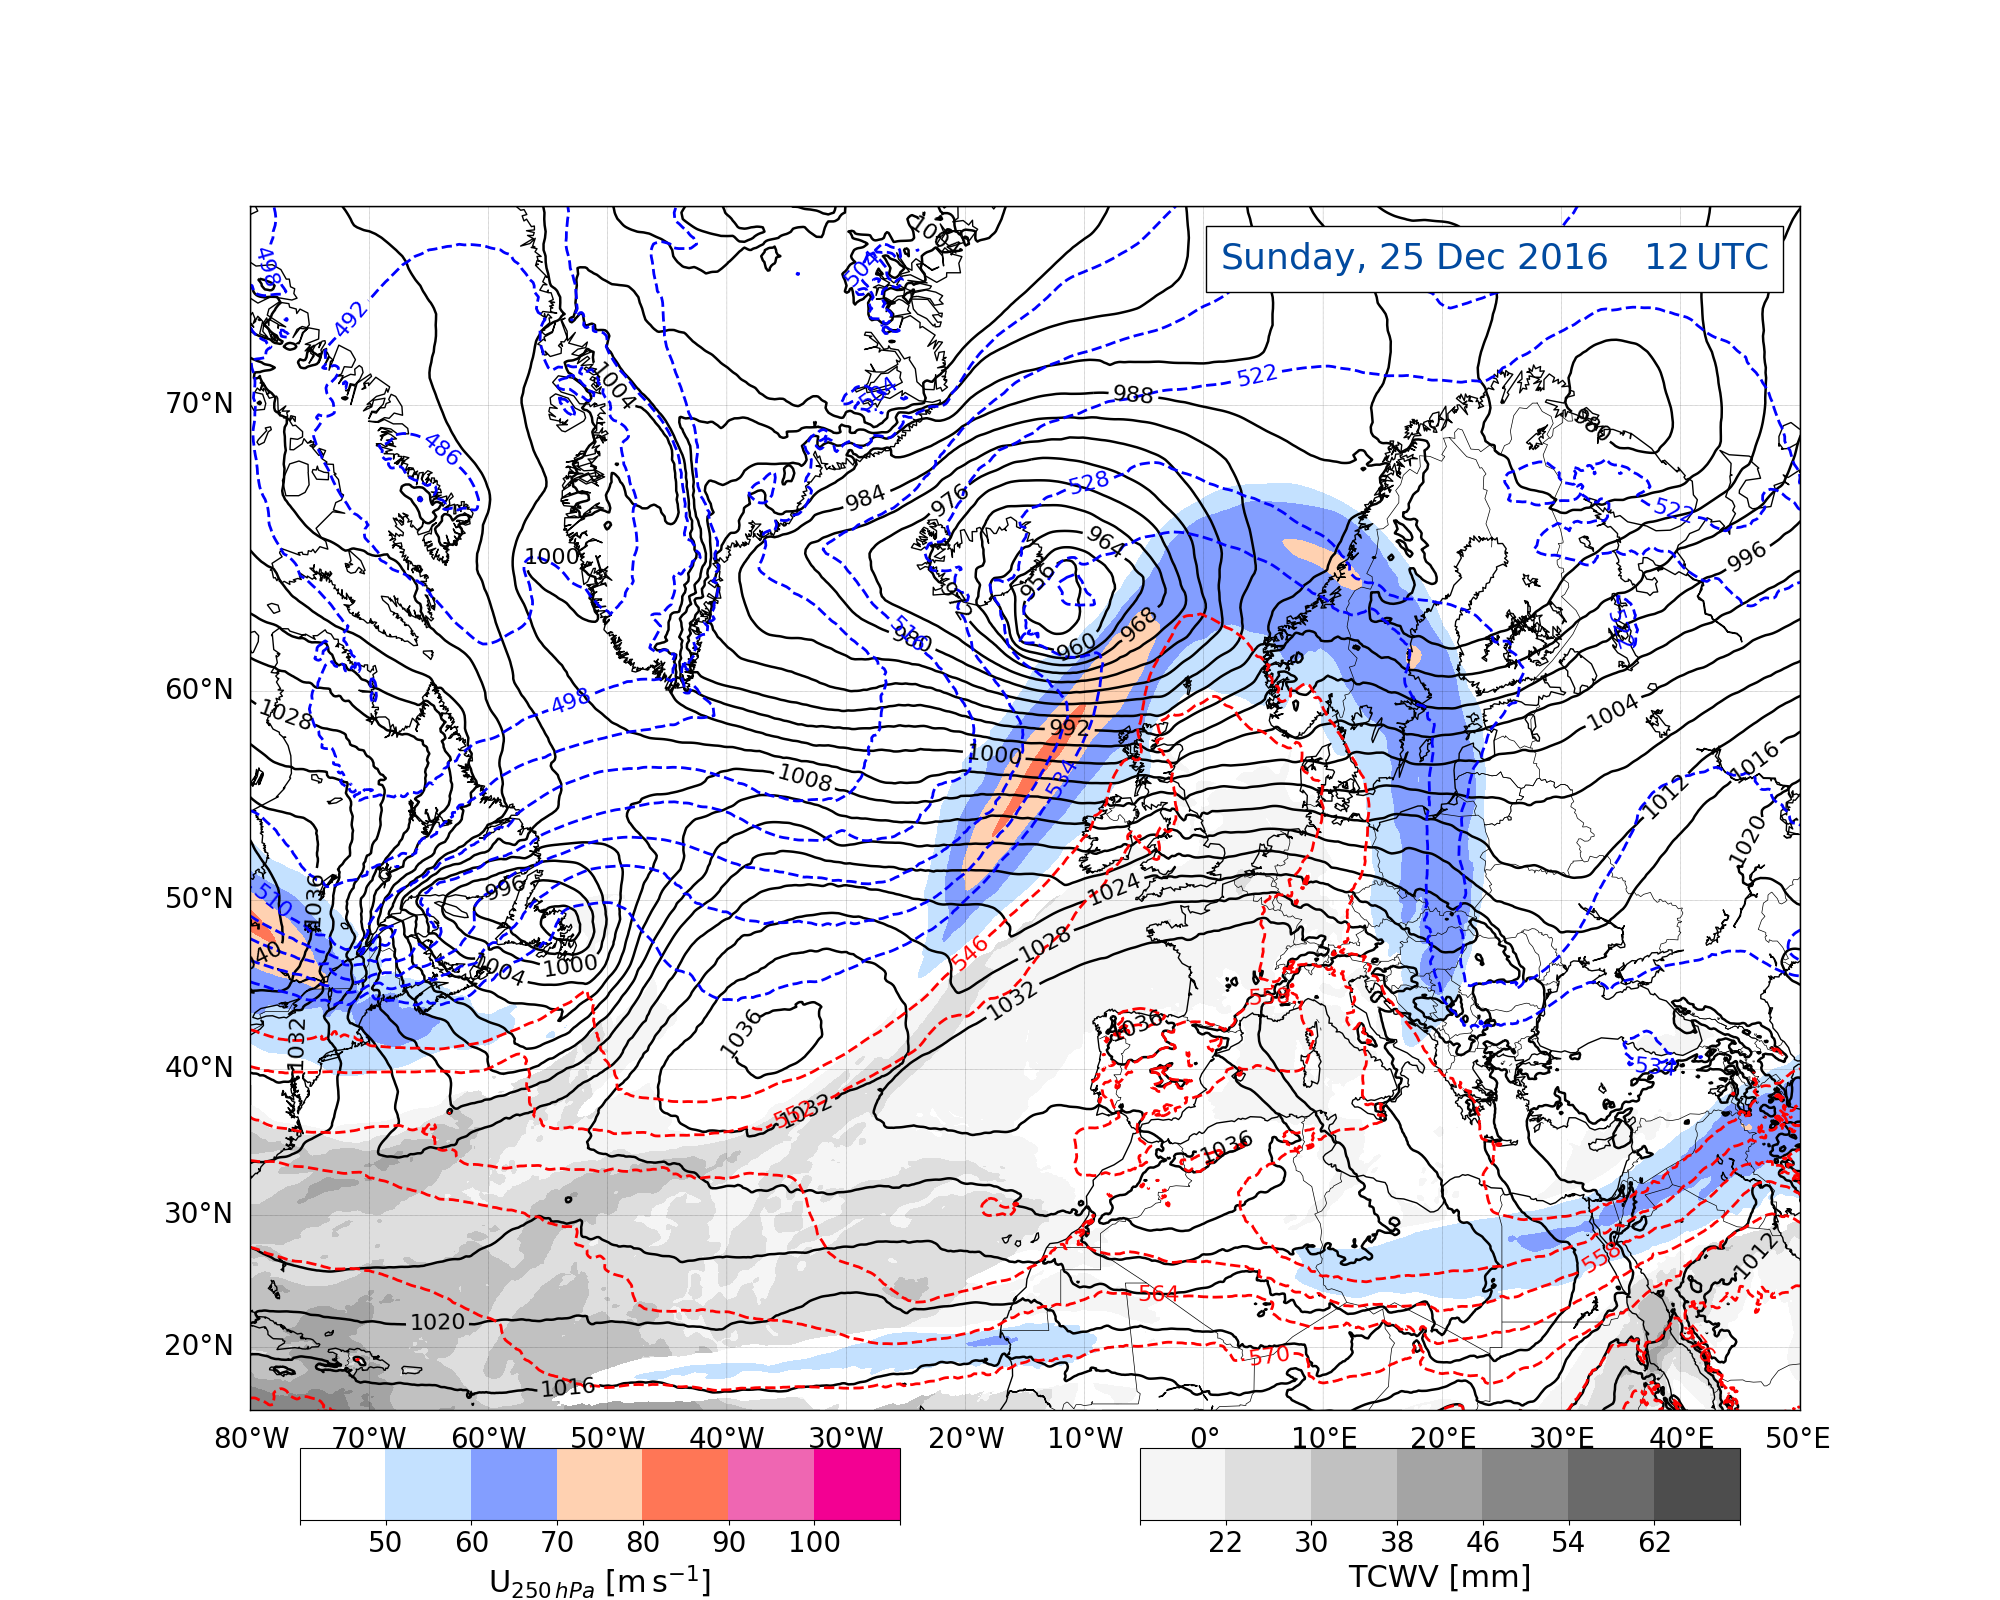
\includegraphics[trim={4.2cm 0cm 4.3cm 5.1cm},clip,
		width=\textwidth]{./fig_Geopot_Jet/20161225_12}
		\caption{} \label{fig:GP25}
	\end{subfigure}
	\begin{subfigure}[b]{0.49\textwidth}
		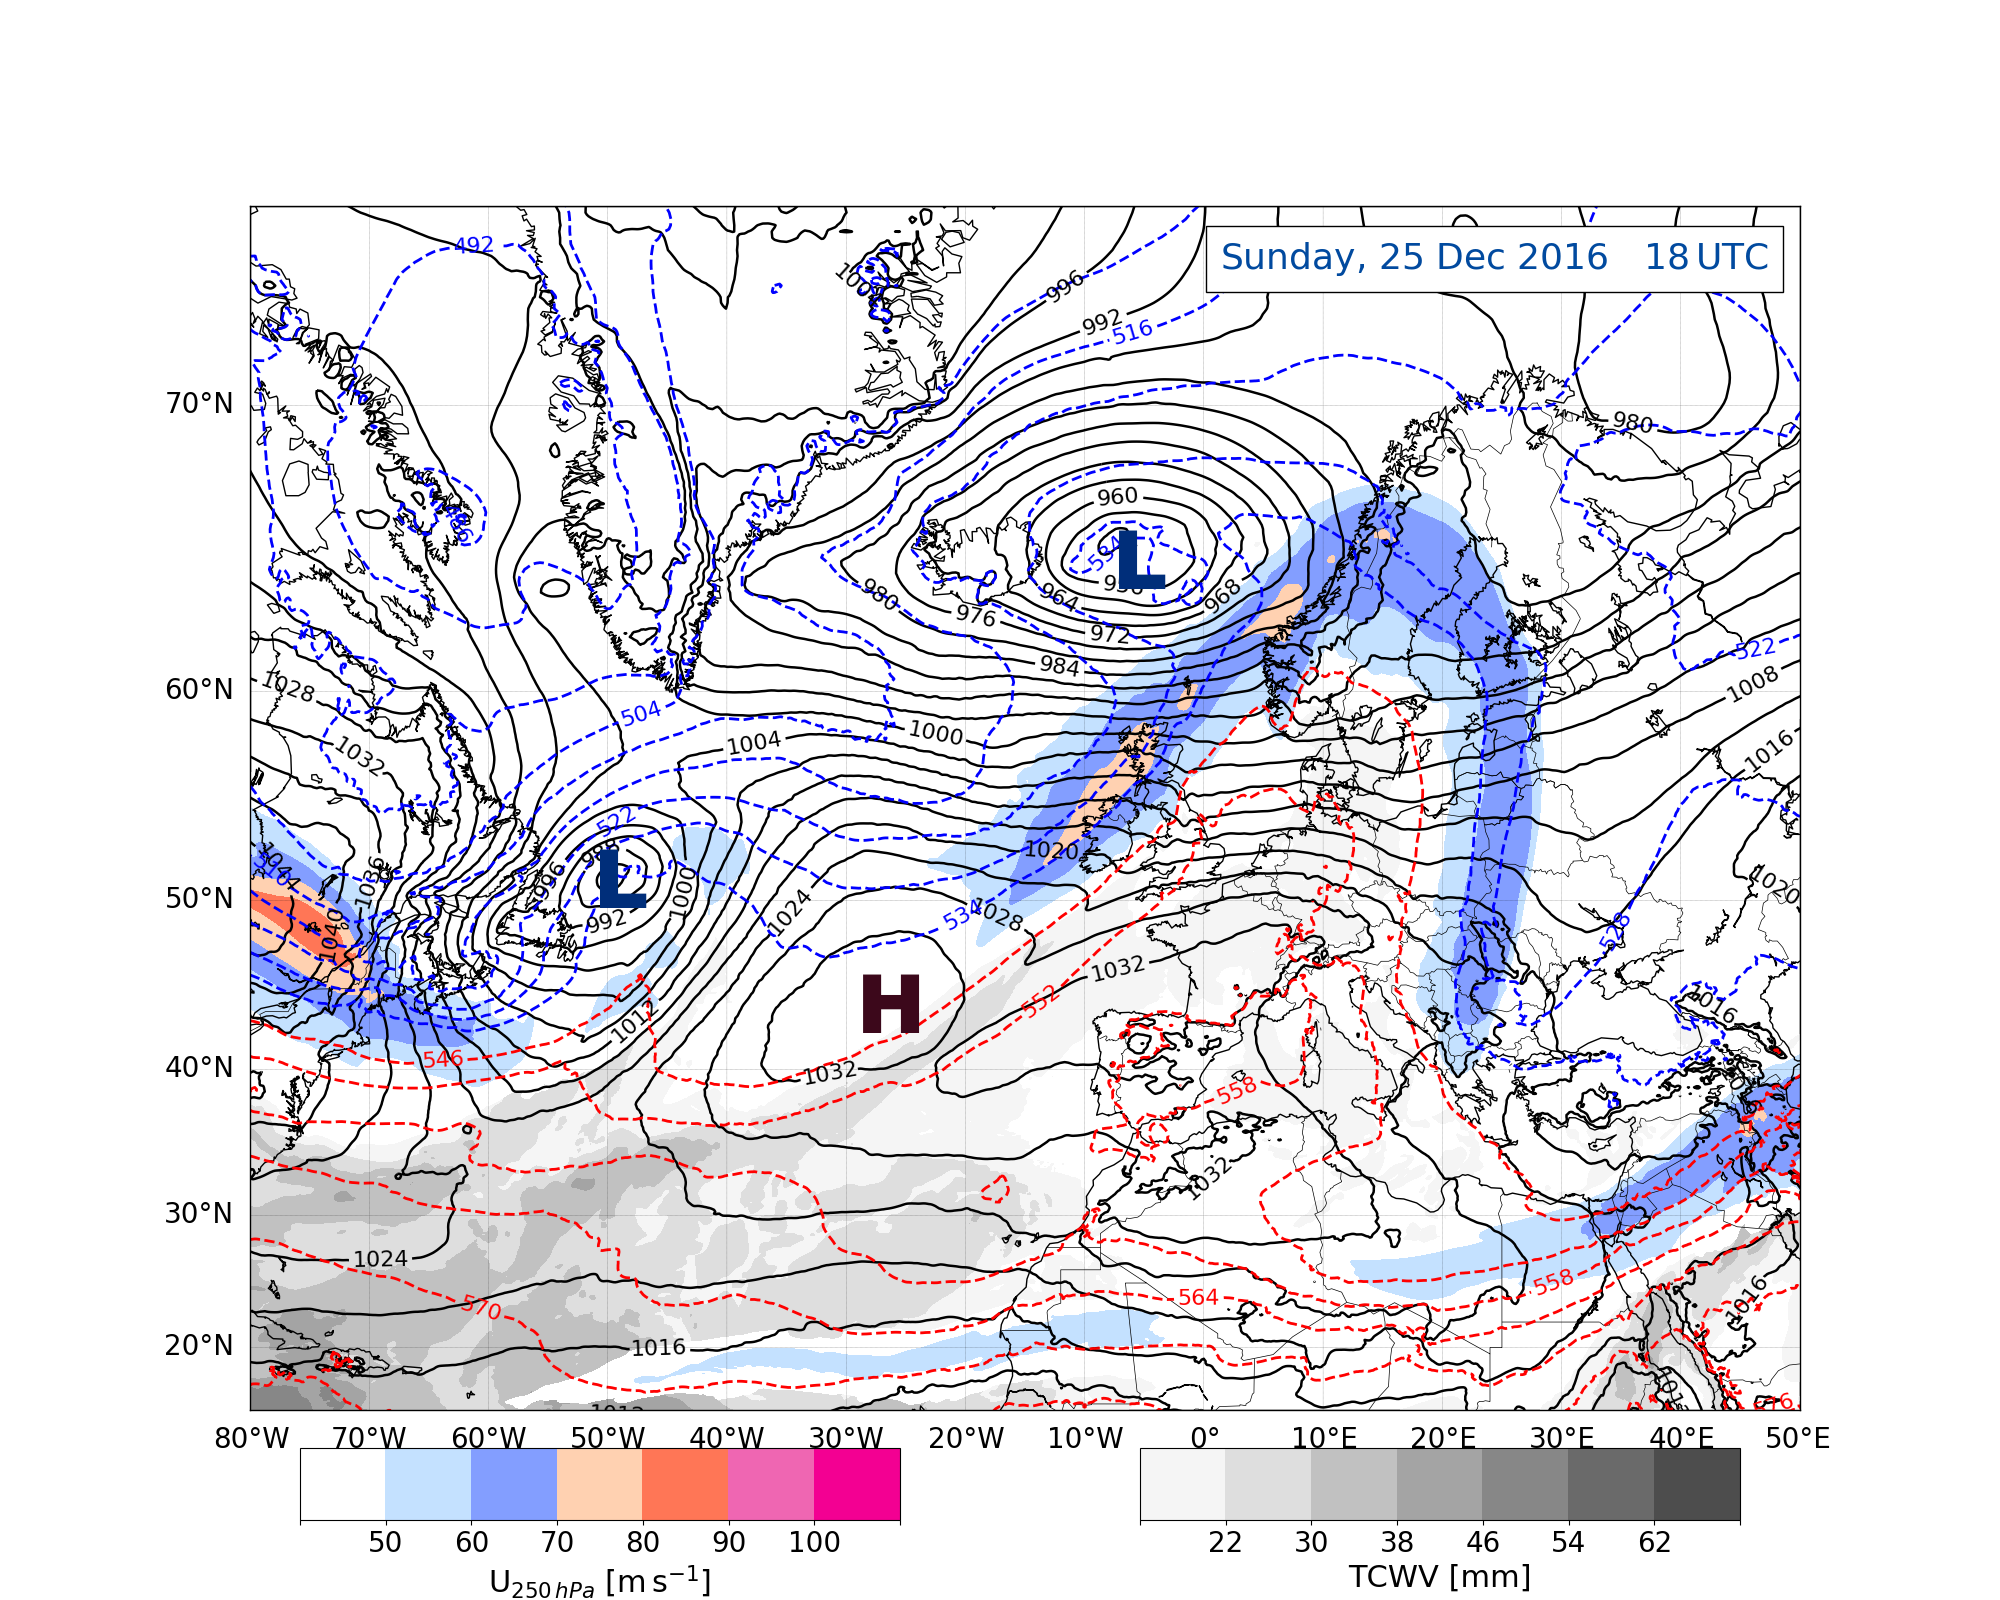
\includegraphics[trim={4.2cm 0cm 4.3cm 5.1cm},clip,
		width=\textwidth]{./fig_Geopot_Jet/20161225_18}
		\caption{} \label{fig:GP25_18}
	\end{subfigure}
	%%% local obs %%%%
	\begin{subfigure}[b]{0.49\textwidth}
		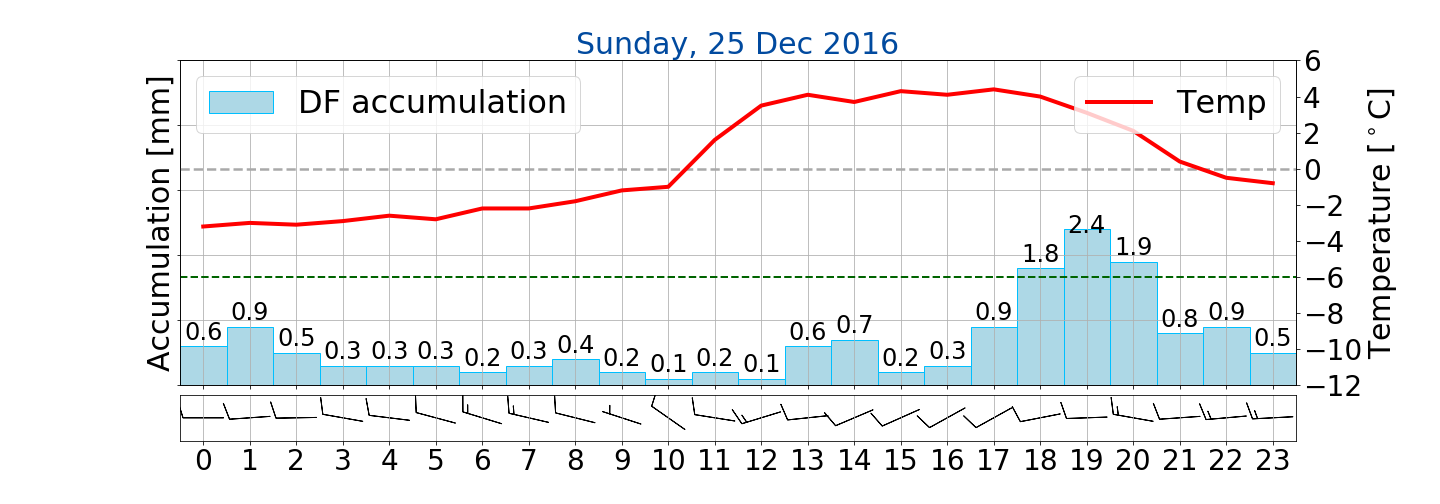
\includegraphics[trim={4.9cm 1.cm 1.5cm 1cm},clip,
		width=\textwidth]{./fig_weathermast/T_P_U_20161225}
		\caption{} \label{fig:TPU25}
	\end{subfigure}
	\caption{\textit{(As \Cref{fig:weather:19}.)} For \SI{25}{\dec} at \SI{12}{\UTC} (\protect\subref{fig:DT25}, \protect\subref{fig:GP25}) and at \SI{18}{\UTC} (\protect\subref{fig:DT25_18}, \protect\subref{fig:GP25_18}).}\label{fig:weather:25}
\end{figure}
%%%%%%%%%%%%%%%%%%%%%%%%%%%%%%%%%%%%%%%%%%%%%%%%%%%%%%%%%%%%%%

\newpage
\subsection*{\SI{26}{\dec}}
%%% 26/12
% 26/06
% Cold front went through
% Norway lies in cold area (@ sfc: blue thickness lines, @ DT: cold anomaly)
% 26/18
% North westerly flow at west coast of Norway
% Conducive for orographic lifting, @ DT: strong low-level vorticity gradient
Within the next twenty-four hours the cold sector comes through Haukeliseter and Norway is covered in cold air (\Cref{fig:DT26}, \subref{fig:GP26_18}). The surface pressure indicates the occlusion of the cyclone and therefore a weakening and dissipation by \SI{18}{\UTC}. A drop in temperature and a change in precipitation phase is observed at Haukeliseter (\Cref{fig:TPU26}).
%%%%%%%%%%%%%%%%%%%%%%%%%%%%%%%%%%%%%%%%%%%%%%%%%%%%%%%%%%%%
\begin{figure}[ht!]%\ContinuedFloat
	\centering
	%%% dyntropo %%%%
	\begin{subfigure}[b]{0.49\textwidth}
		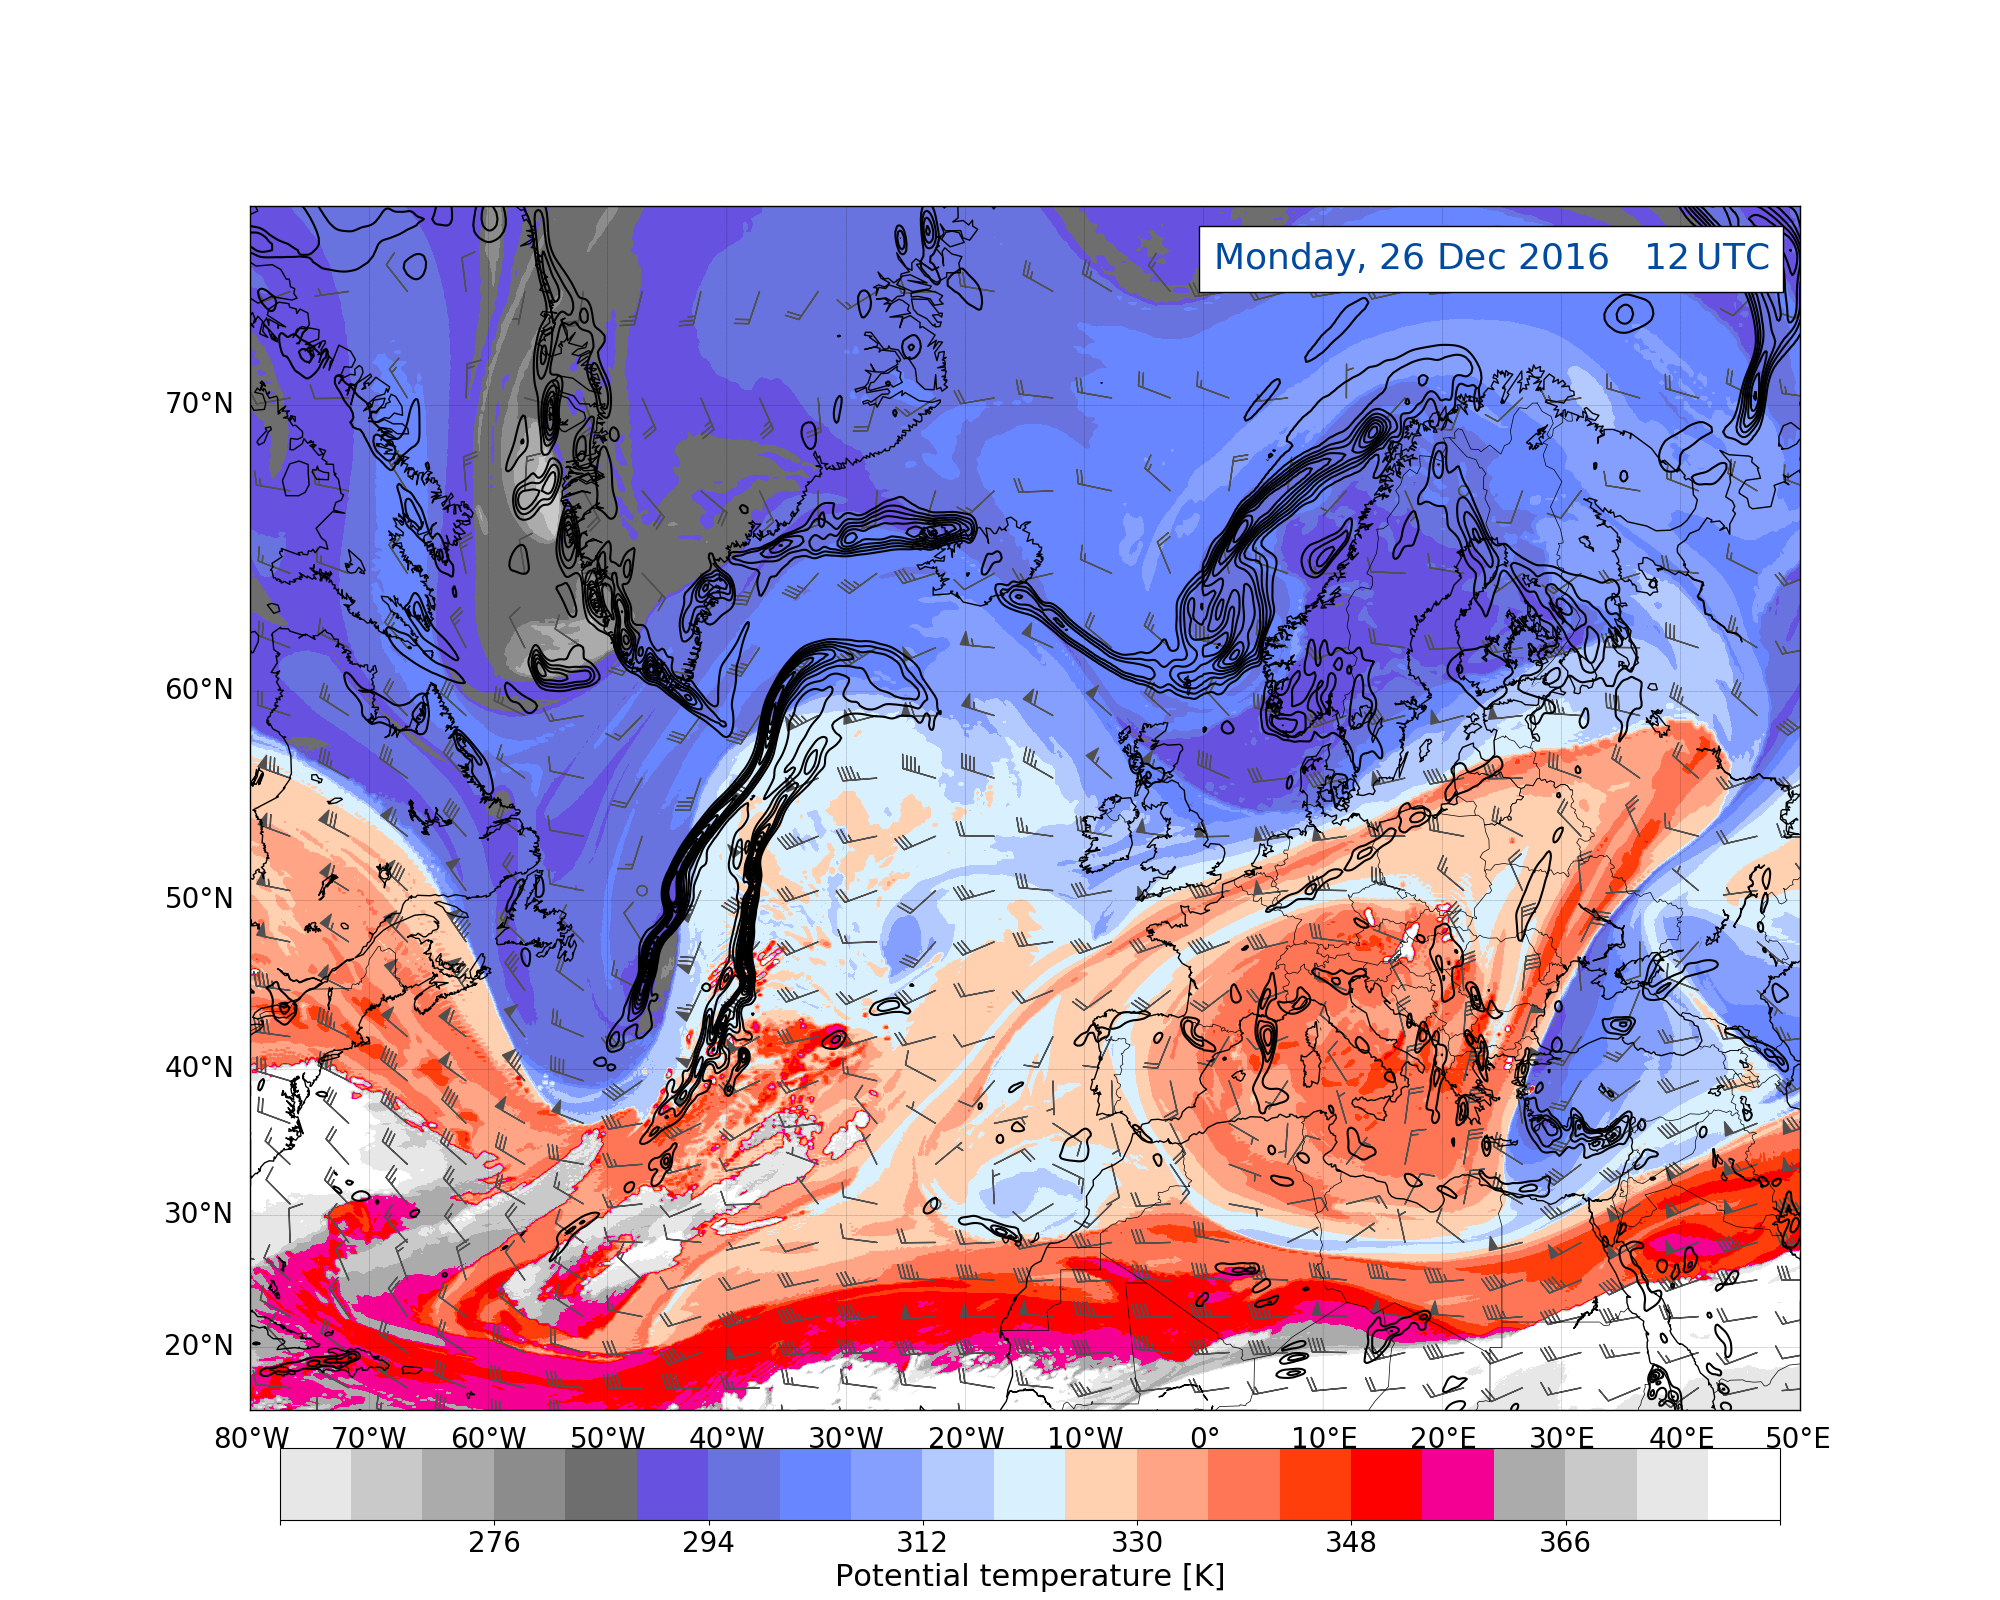
\includegraphics[trim={4.2cm 0cm 4.3cm 5.1cm},clip,
		width=\textwidth]{./fig_DynTropo/20161226_12}
		\caption{} \label{fig:DT26}
	\end{subfigure}
	\begin{subfigure}[b]{0.49\textwidth}
		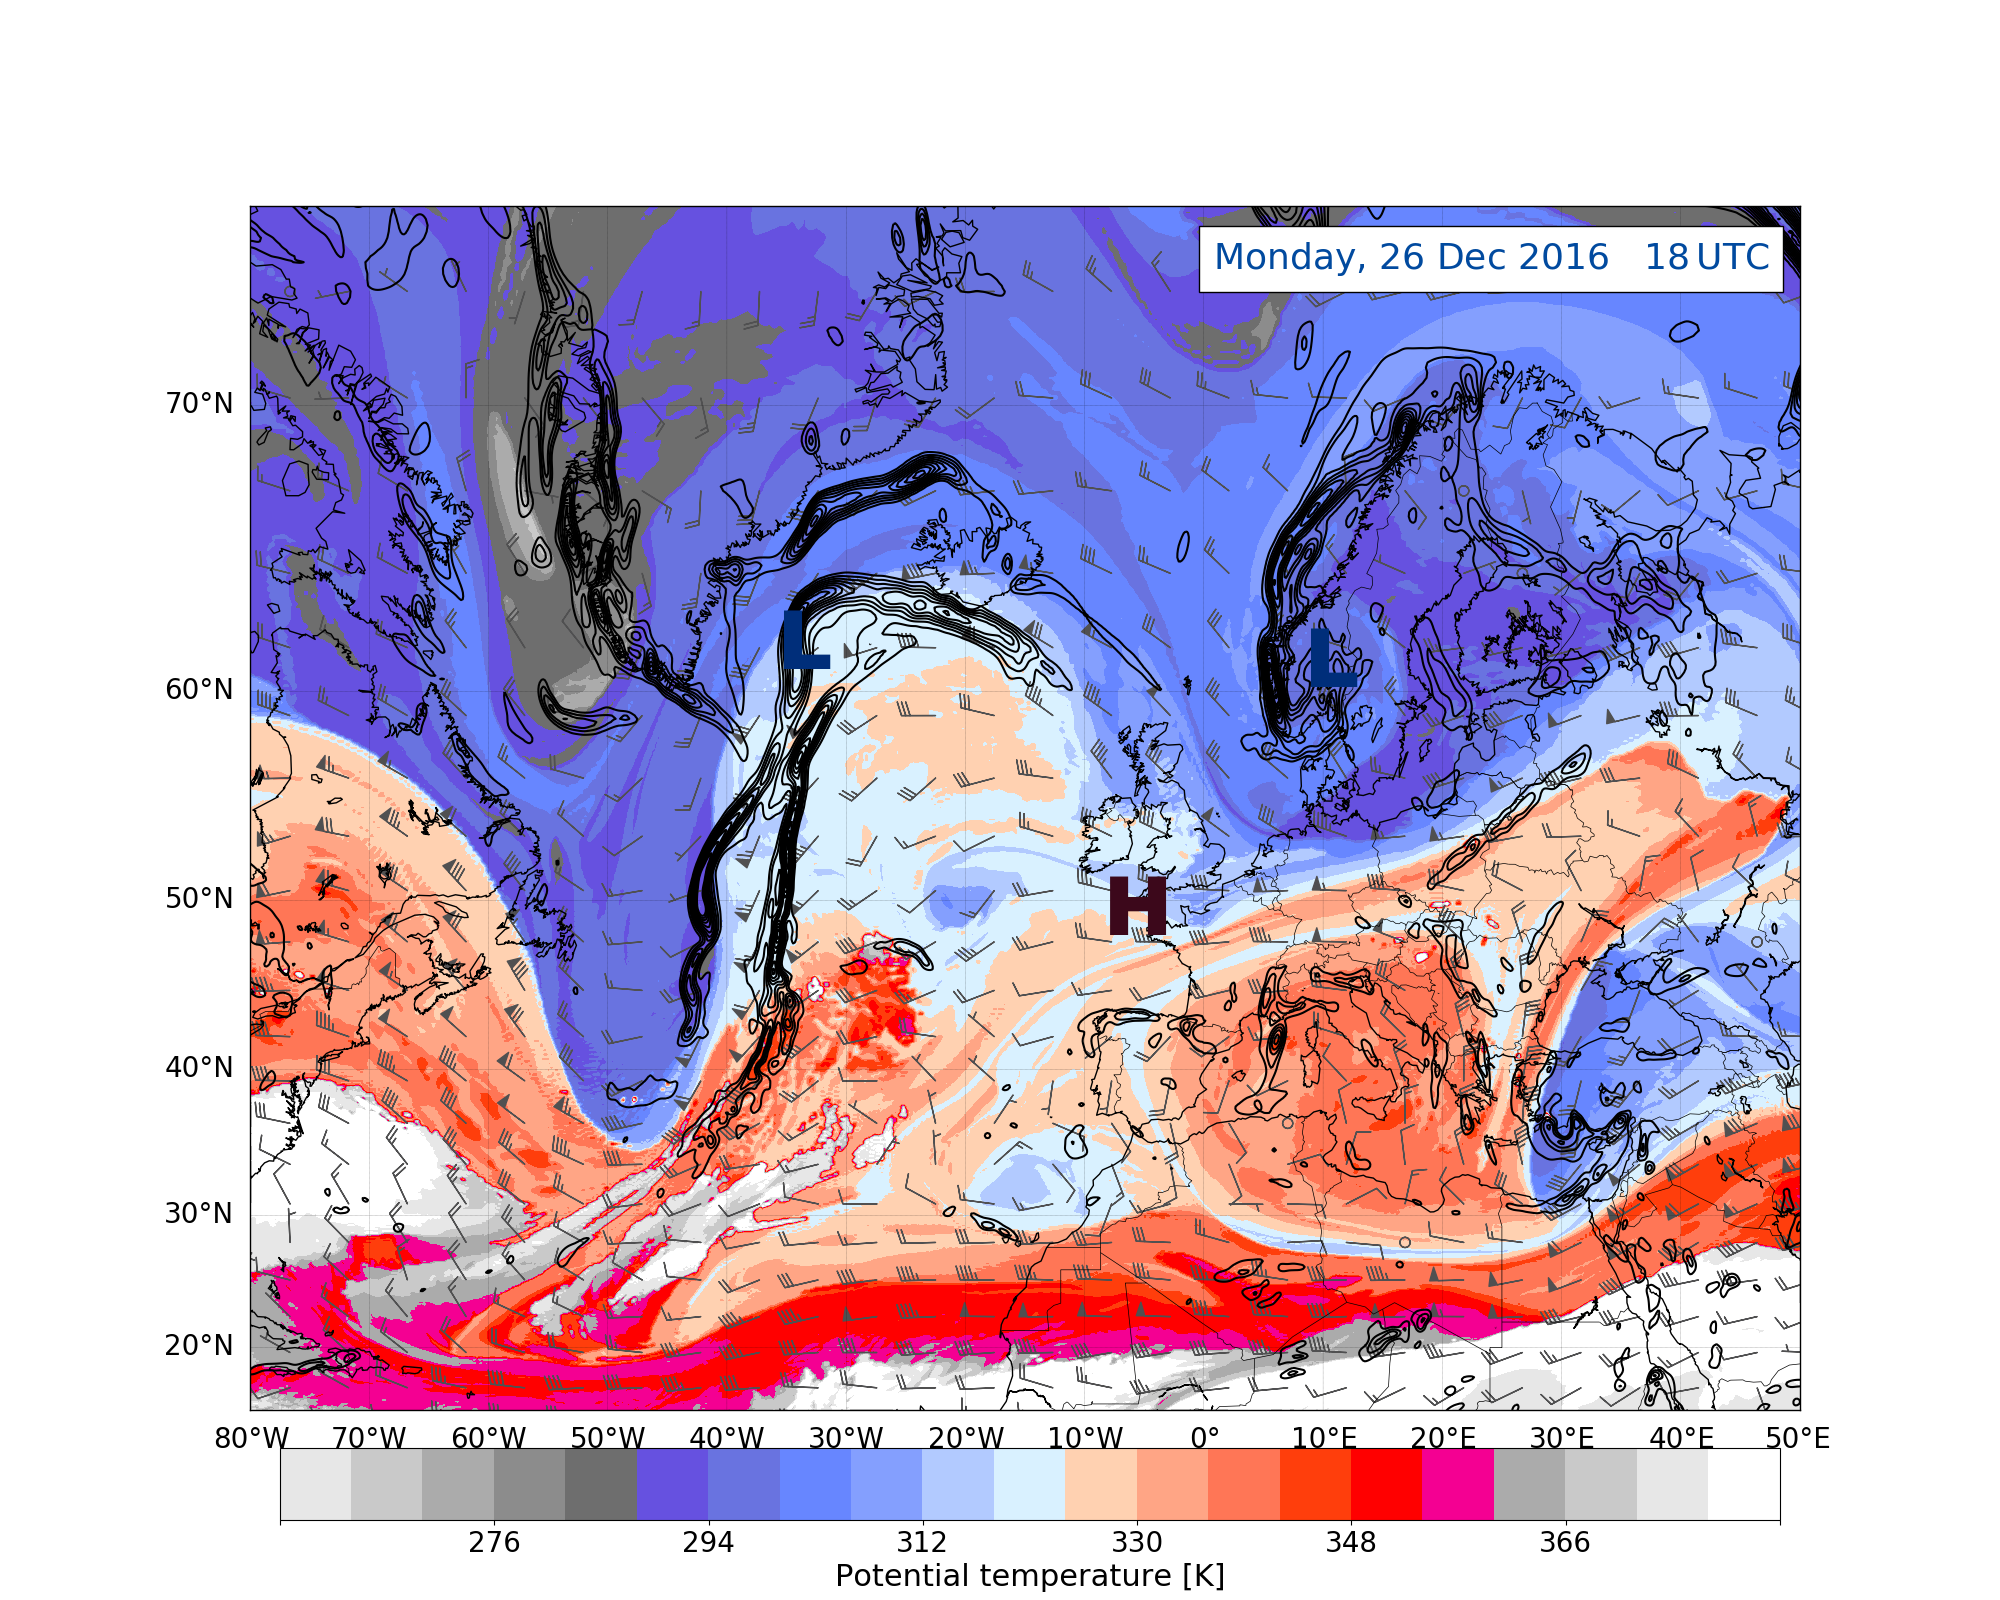
\includegraphics[trim={4.2cm 0cm 4.3cm 5.1cm},clip,
		width=\textwidth]{./fig_DynTropo/20161226_18}
		\caption{} \label{fig:DT26_18}
	\end{subfigure}
	%%% geopot %%%%
	\begin{subfigure}[b]{0.49\textwidth}
		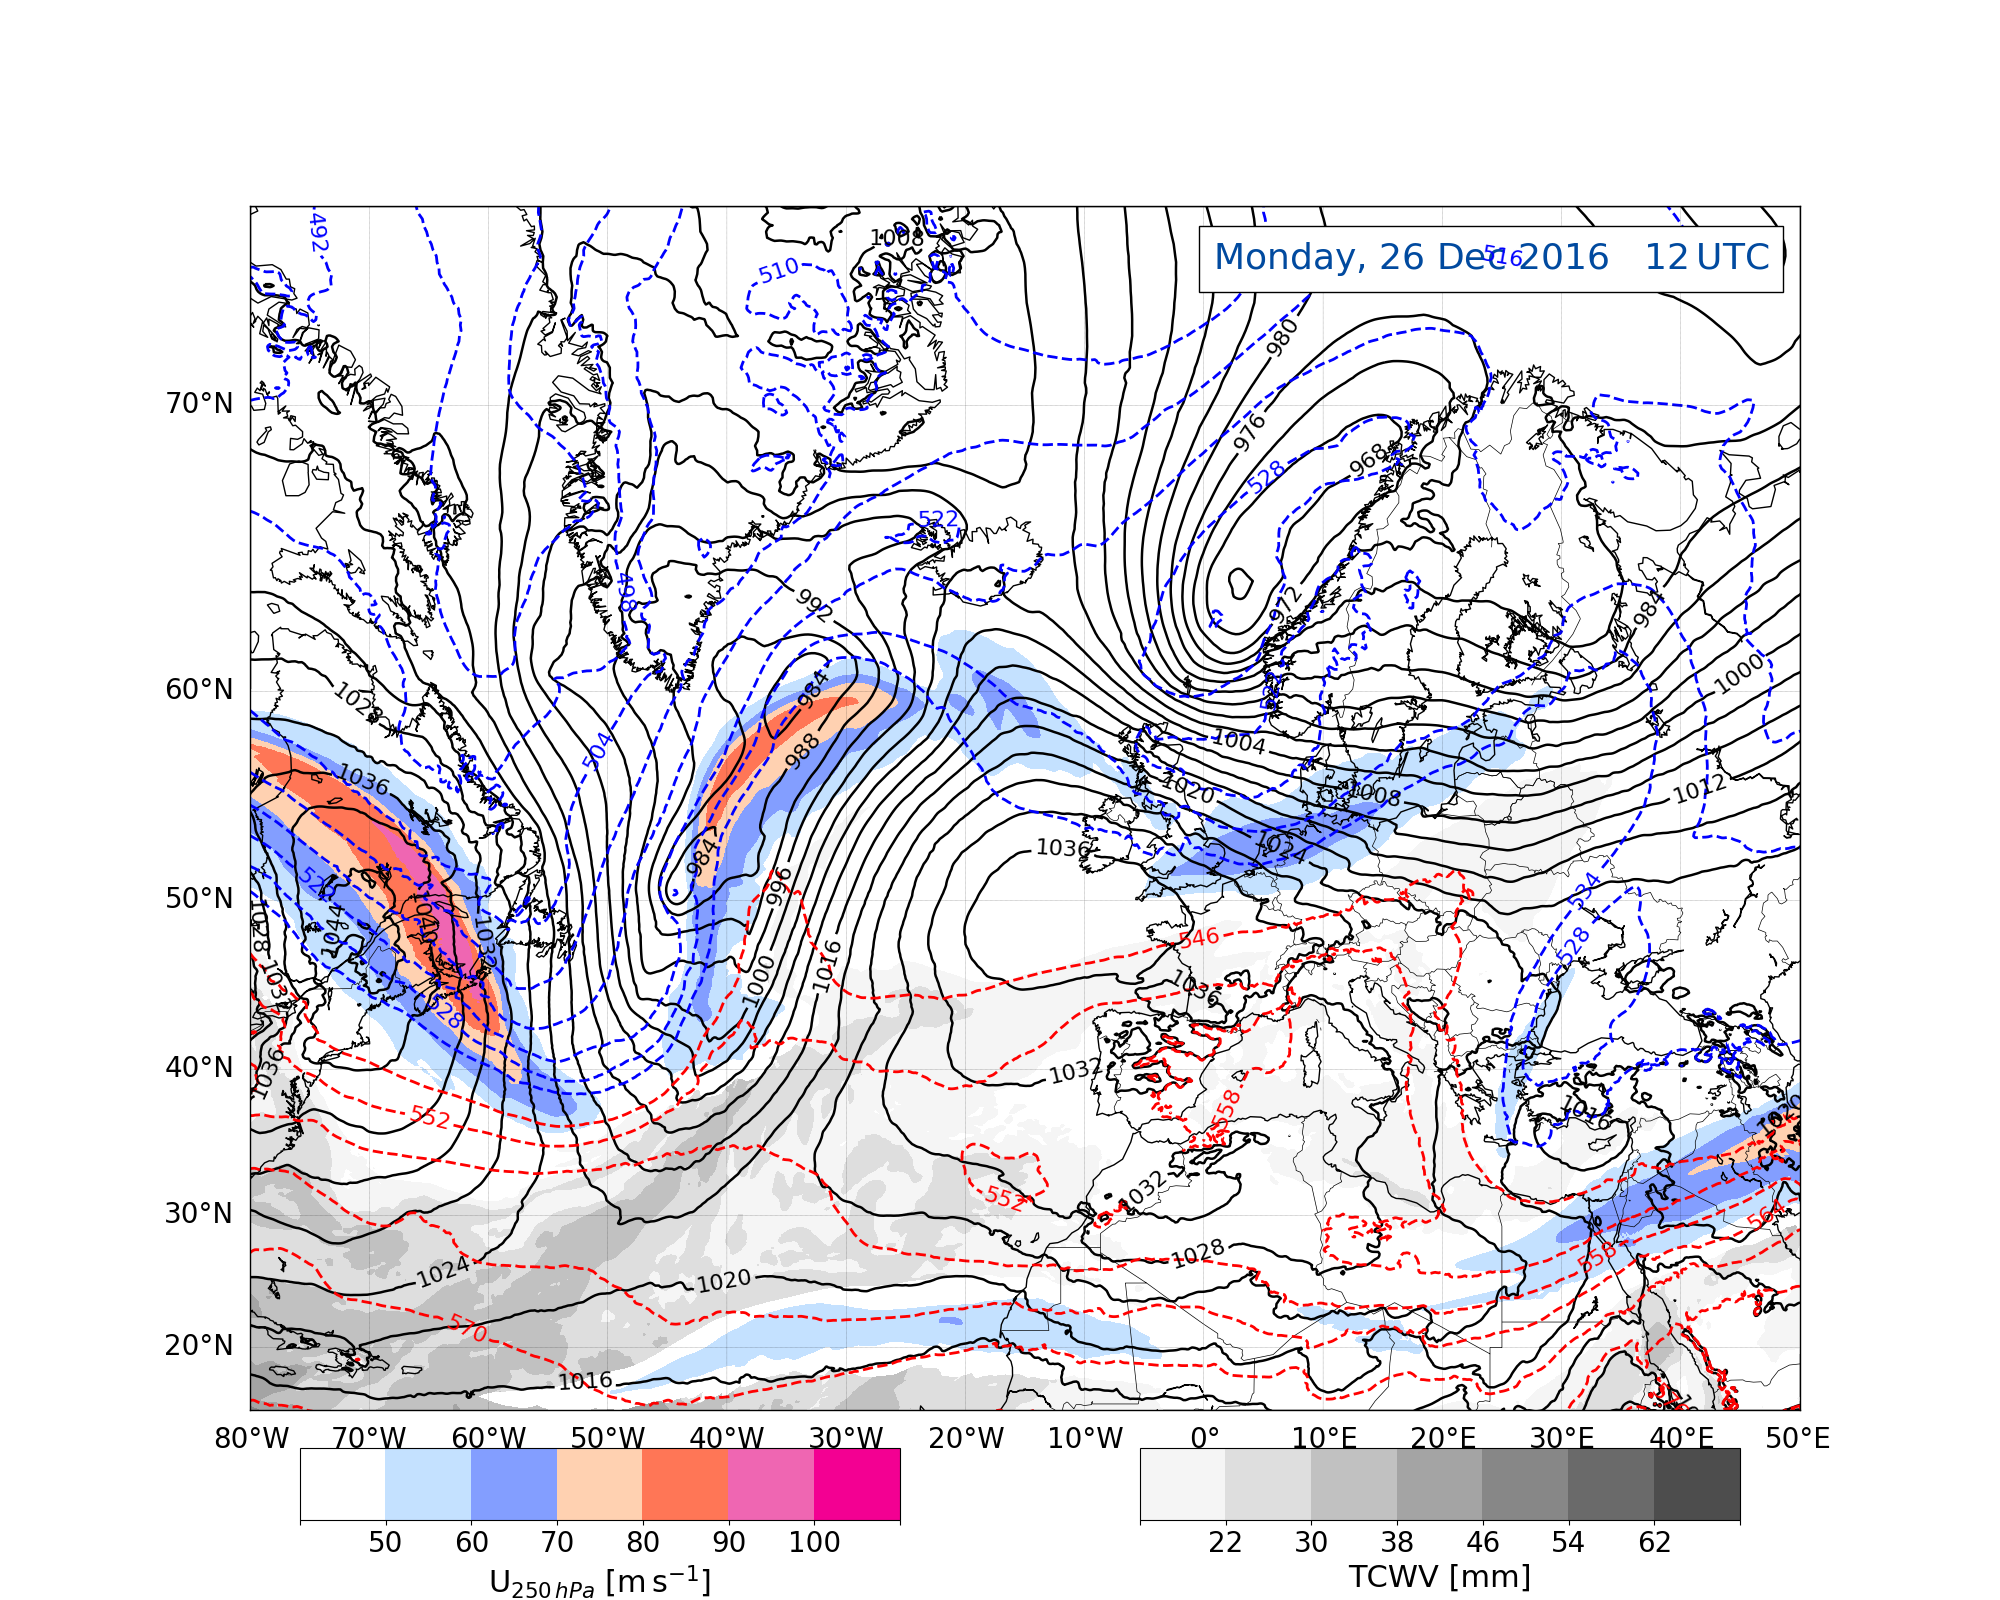
\includegraphics[trim={4.2cm 0cm 4.3cm 5.1cm},clip,
		width=\textwidth]{./fig_Geopot_Jet/20161226_12}
		\caption{} \label{fig:GP26}
	\end{subfigure}
	\begin{subfigure}[b]{0.49\textwidth}
		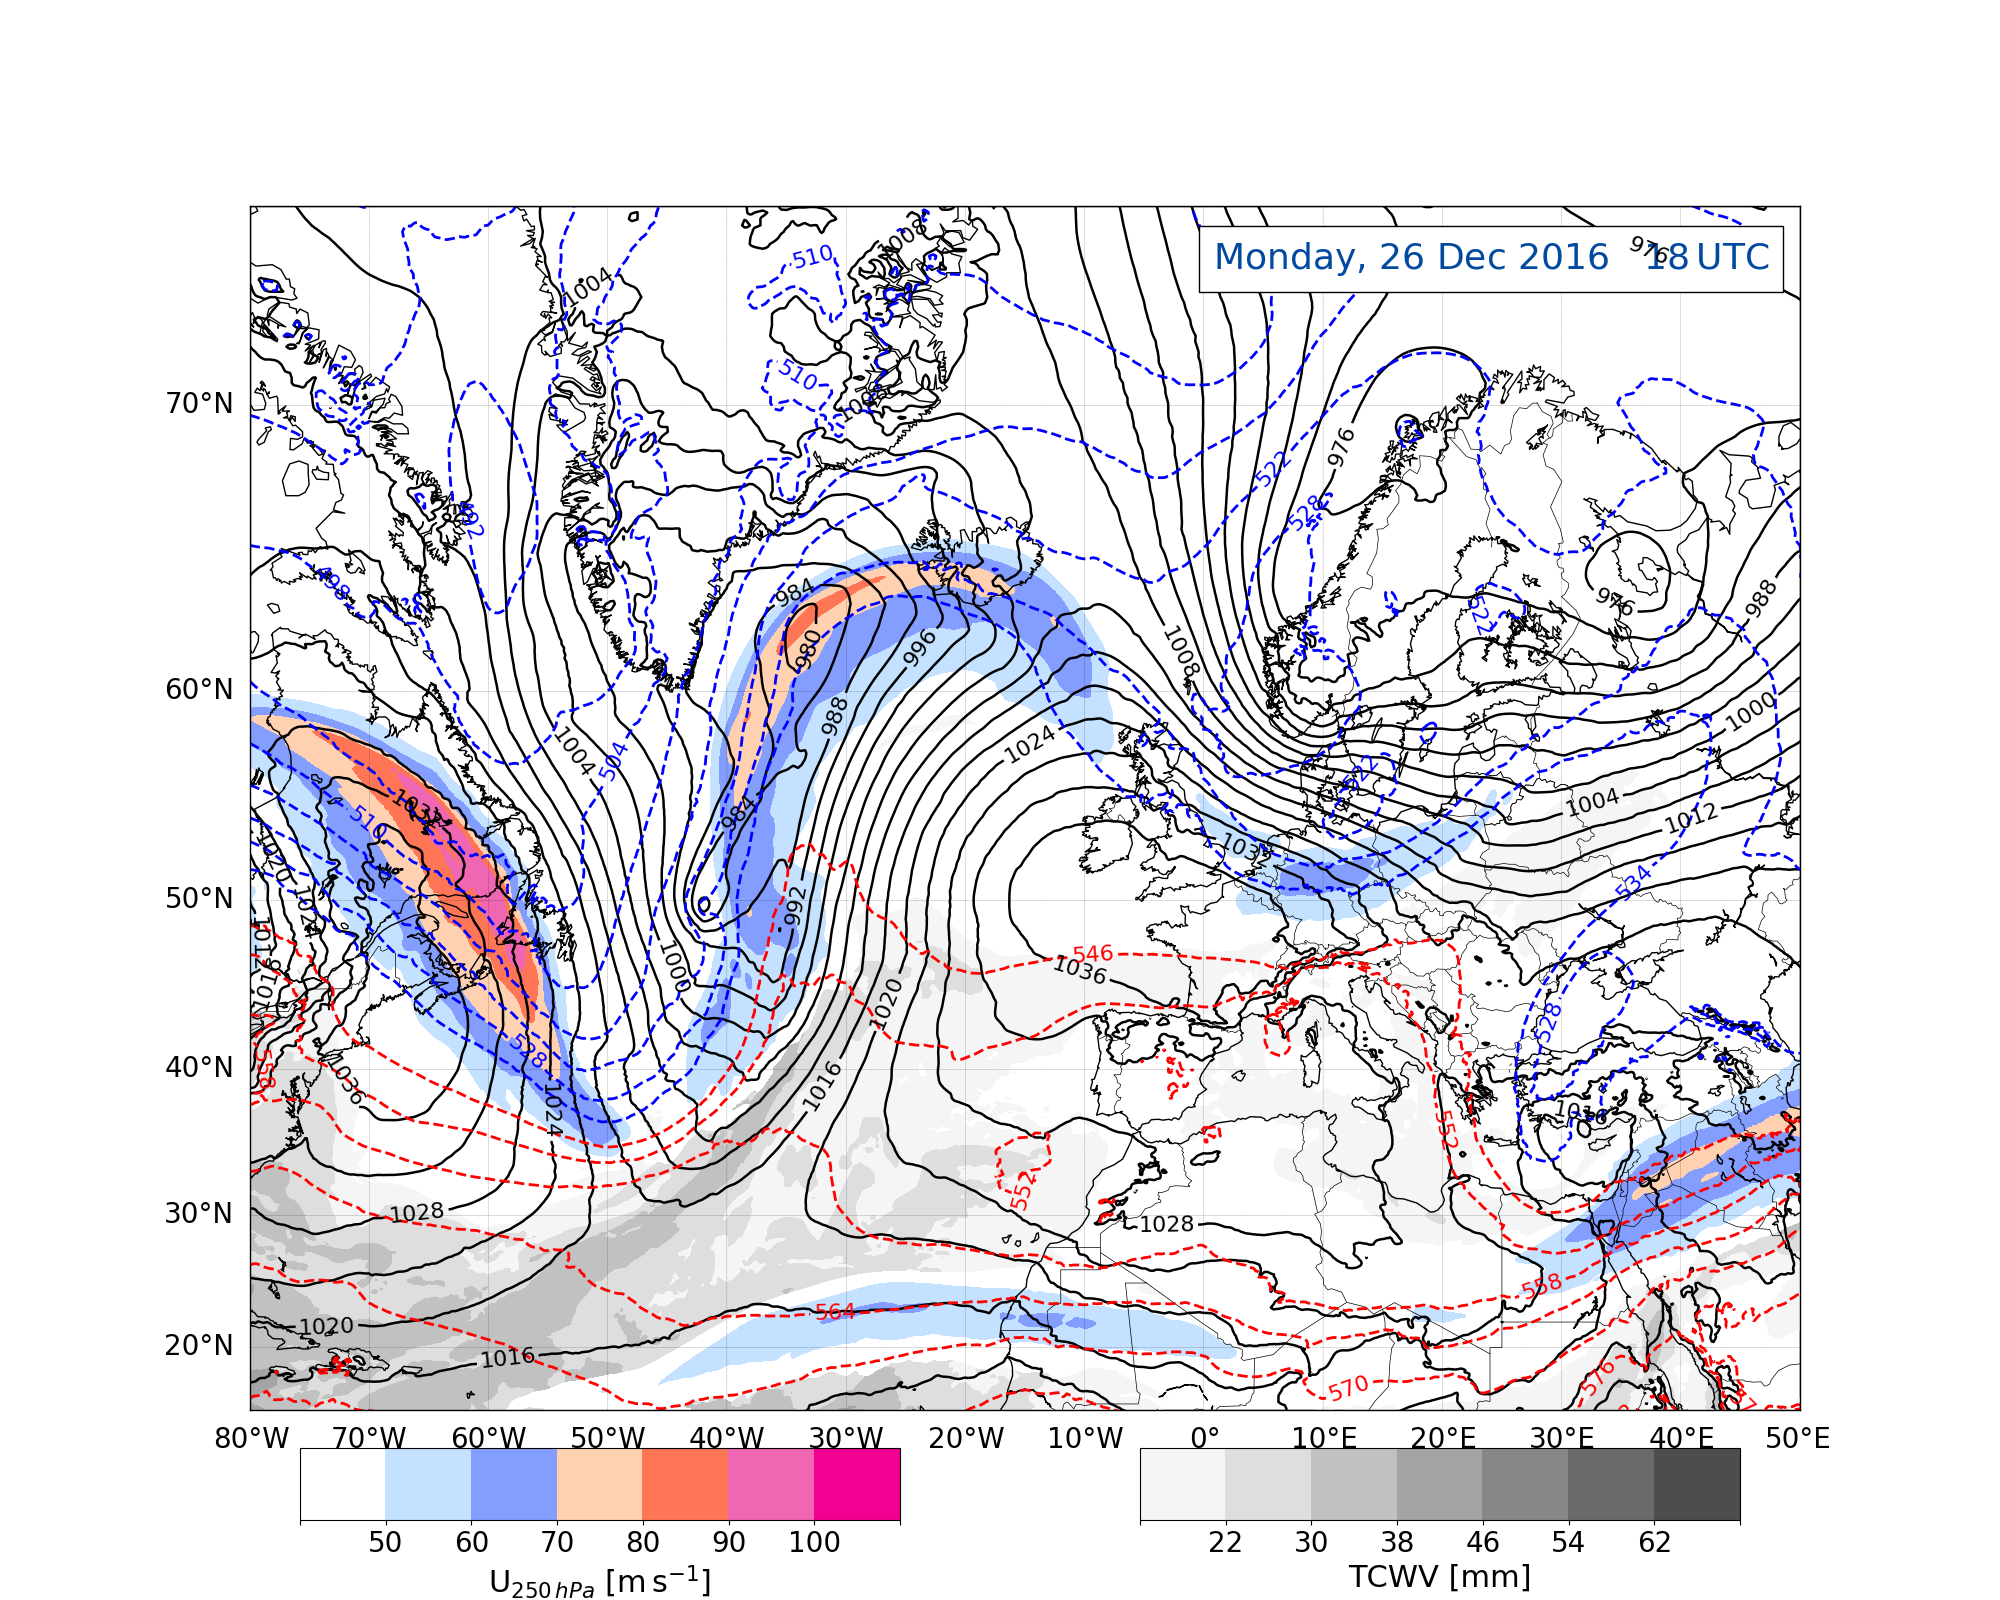
\includegraphics[trim={4.2cm 0cm 4.3cm 5.1cm},clip,
		width=\textwidth]{./fig_Geopot_Jet/20161226_18}
		\caption{} \label{fig:GP26_18}
	\end{subfigure}
	%%% local obs %%%%
	\begin{subfigure}[b]{0.49\textwidth}
		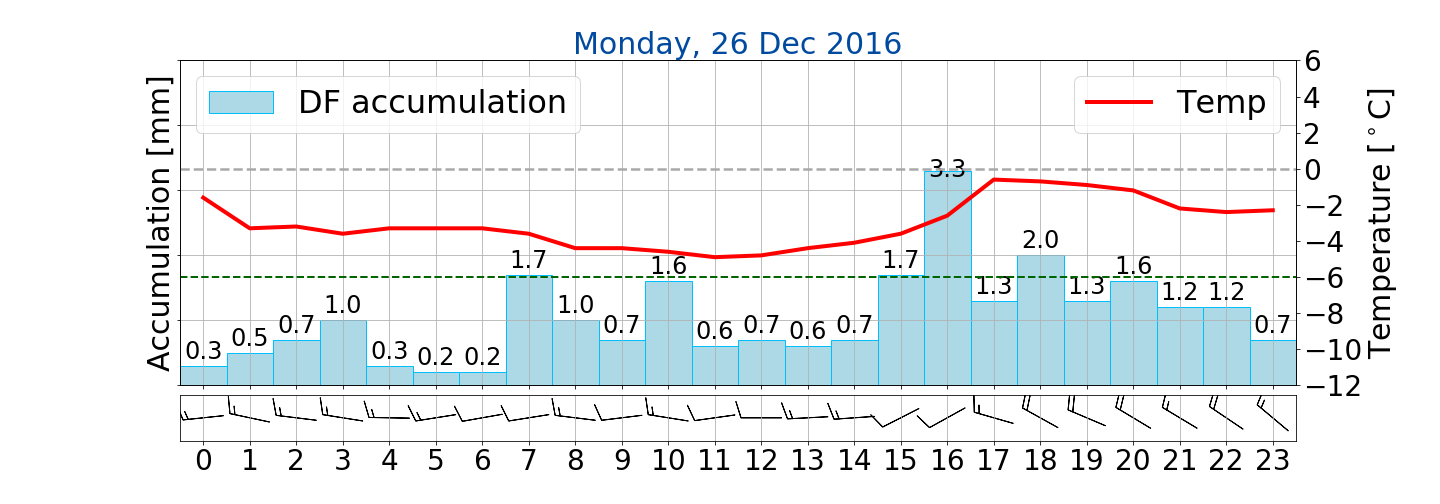
\includegraphics[trim={4.9cm 1.cm 1.5cm 1cm},clip,
		width=\textwidth]{./fig_weathermast/T_P_U_20161226}
		\caption{} \label{fig:TPU26}
	\end{subfigure}
	\caption{\textit{(As \Cref{fig:weather:19}.)} For \SI{26}{\dec} at \SI{12}{\UTC} (\protect\subref{fig:DT26}, \protect\subref{fig:GP26}) and at \SI{18}{\UTC} (\protect\subref{fig:DT26_18}, \protect\subref{fig:GP26_18}).}\label{fig:weather:26}
\end{figure}
%%%%%%%%%%%%%%%%%%%%%%%%%%%%%%%%%%%%%%%%%%%%%%%%%%%%%%%%%%%%%

% %%%%%%%%%%%%%%%%%%%%%%%%%%%%%%%%%%%%%%%%%%%%%%%%%%%%%%%%%%%%%%
% % \subsection*{\SI{27}{\dec}}
% % %%% 27/12
% % \noindent
% % The images of \SI{27}{\dec} show that the storm passed and disappeared. Southern Norway lies in cold air (\Cref{fig:DT27}), but on the right exit region of the jet ($\rightarrow$ sinking motion of cold air), compare \ref{fig:GP27}. A small amount of moisture is present (\Cref{fig:AR27}). Because of the wind change from west to north-west follows that orographic lifting is not present and the precipitation amount decreases at the end of the storm. 



